\documentclass[compress]{beamer}
\usepackage{ifthen,verbatim}

\newcommand{\isnote}{}
\xdefinecolor{lightyellow}{rgb}{1.,1.,0.25}
\xdefinecolor{darkblue}{rgb}{0.1,0.1,0.7}

%% Uncomment this to get annotations
%% \def\notes{\addtocounter{page}{-1}
%%            \renewcommand{\isnote}{*}
%% 	   \beamertemplateshadingbackground{lightyellow}{white}
%%            \begin{frame}
%%            \frametitle{Notes for the previous page (page \insertpagenumber)}
%%            \itemize}
%% \def\endnotes{\enditemize
%% 	      \end{frame}
%%               \beamertemplateshadingbackground{white}{white}
%%               \renewcommand{\isnote}{}}

%% Uncomment this to not get annotations
\def\notes{\comment}
\def\endnotes{\endcomment}

\setbeamertemplate{navigation symbols}{}
\setbeamertemplate{headline}{\mbox{ } \hfill
\begin{minipage}{5.5 cm}
\vspace{-0.75 cm} \small
\end{minipage} \hfill
\begin{minipage}{4.5 cm}
\vspace{-0.75 cm} \small
\begin{flushright}
\ifthenelse{\equal{\insertpagenumber}{1}}{}{Jim Pivarski \hspace{0.2 cm} \insertpagenumber\isnote/\pageref{numpages}}
\end{flushright}
\end{minipage}\mbox{\hspace{0.2 cm}}\includegraphics[height=1 cm]{../cmslogo} \hspace{0.1 cm} \includegraphics[height=1 cm]{../tamulogo} \hspace{0.01 cm} \vspace{-1.05 cm}}

\begin{document}
\begin{frame}
\vfill
\begin{center}
\textcolor{darkblue}{\Large Testing Alignment with Residuals-Differences}

\vfill
\begin{columns}
\column{0.3\linewidth}
\begin{center}
\large
\textcolor{darkblue}{Jim Pivarski}

\vspace{0.2 cm}
Alexei Safonov
\end{center}
\end{columns}

\begin{columns}
\column{0.3\linewidth}
\begin{center}
\scriptsize
{\it Texas A\&M University}
\end{center}
\end{columns}

\vfill
 2 June, 2009

\end{center}
\end{frame}

%% \begin{notes}
%% \item This is the annotated version of my talk.
%% \item If you want the version that I am presenting, download the one
%% labeled ``slides'' on Indico (or just ignore these yellow pages).
%% \item The annotated version is provided for extra detail and a written
%% record of comments that I intend to make orally.
%% \item Yellow notes refer to the content on the {\it previous} page.
%% \item All other slides are identical for the two versions.
%% \end{notes}

\small

\begin{frame}
\frametitle{Reminder of the method}

\begin{columns}
\column{0.3\linewidth}
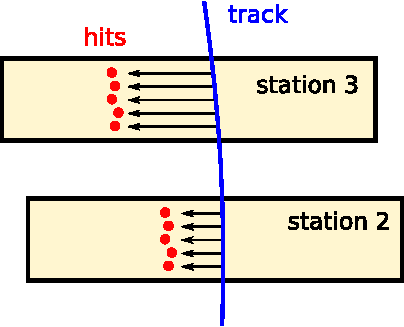
\includegraphics[width=\linewidth]{residuals_difference.pdf}

\column{0.7\linewidth}
\begin{itemize}
\item Plot difference of residuals on same track from different
  stations:

\mbox{\hspace{-1.3 cm} \scriptsize (station~3 track $-$ station~3 hit) $-$ (station~2 track $-$ station~2 hit)}
\end{itemize}
\end{columns}

\vfill
\textcolor{darkblue}{\large Similarity to segment extrapolation}

\begin{itemize}
\item Represents {\it relative} position of the chambers, not how either relates to the tracker (that part cancels)
\item Introduces new information not used in alignment: higher precision in position ($x$) differences and angle ($\phi_y$) differences
\end{itemize}

\vfill
\textcolor{darkblue}{\large Differences from segment extrapolation}

\begin{itemize}
\item Propagates with full CMSSW propagator, not a straight line
\begin{itemize}
\item curvature of the track determined by tracker $p_T$ measurement
\end{itemize}
\item Can't be extended to tracks that don't point to tracker or 0~T data
\end{itemize}
\end{frame}

\begin{frame}
\frametitle{Differences by sector: $x$}
\begin{itemize}
\item Differences between stations 3 and 4 in wheel 1
\item Distributions have tails: fit with Gaussian $\otimes$ Lorentzian
\begin{itemize}
\item doesn't matter: fit result (circles, next pages) are nearly equal to the mean (stars), usually overlapping
\end{itemize}
\end{itemize}

\begin{columns}
\column{0.7\linewidth}
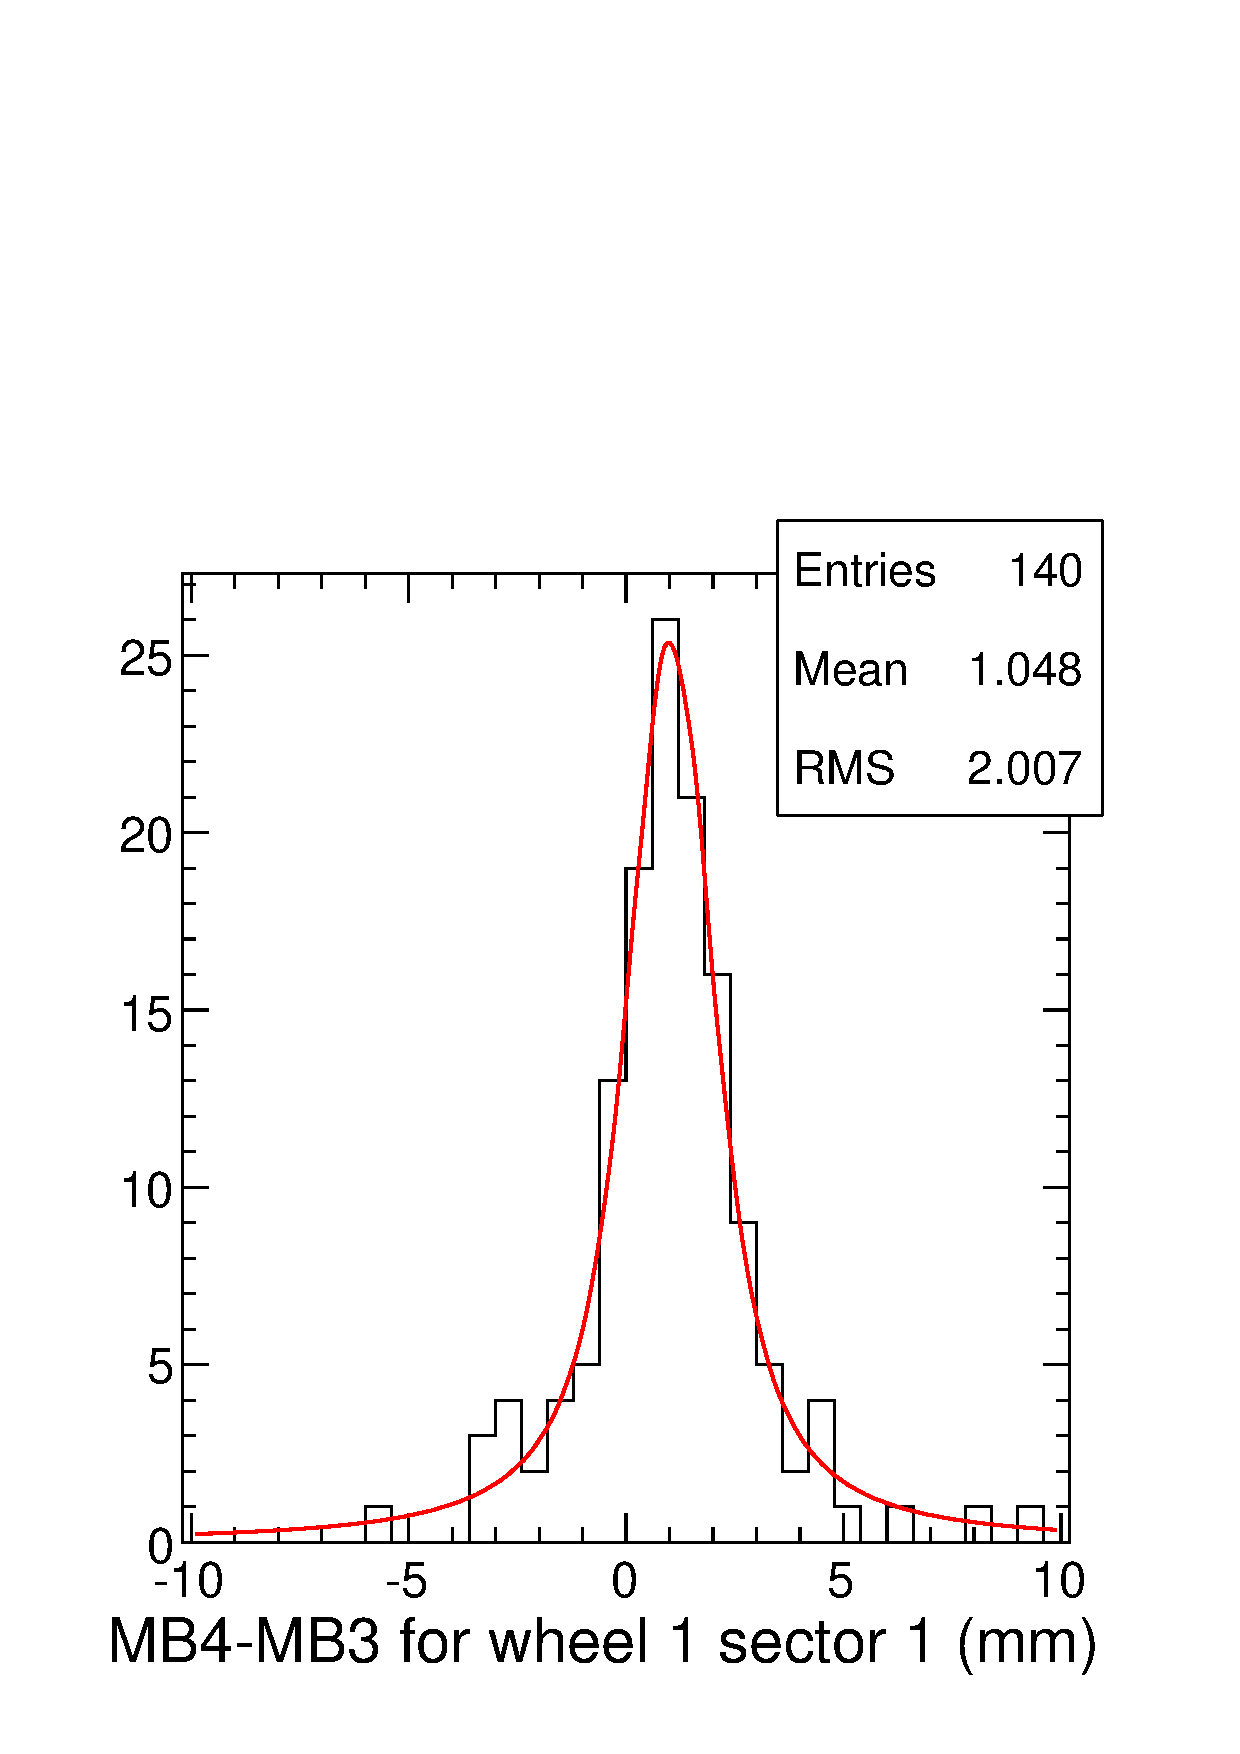
\includegraphics[width=0.25\linewidth]{diffindivx_1_34_1.pdf}
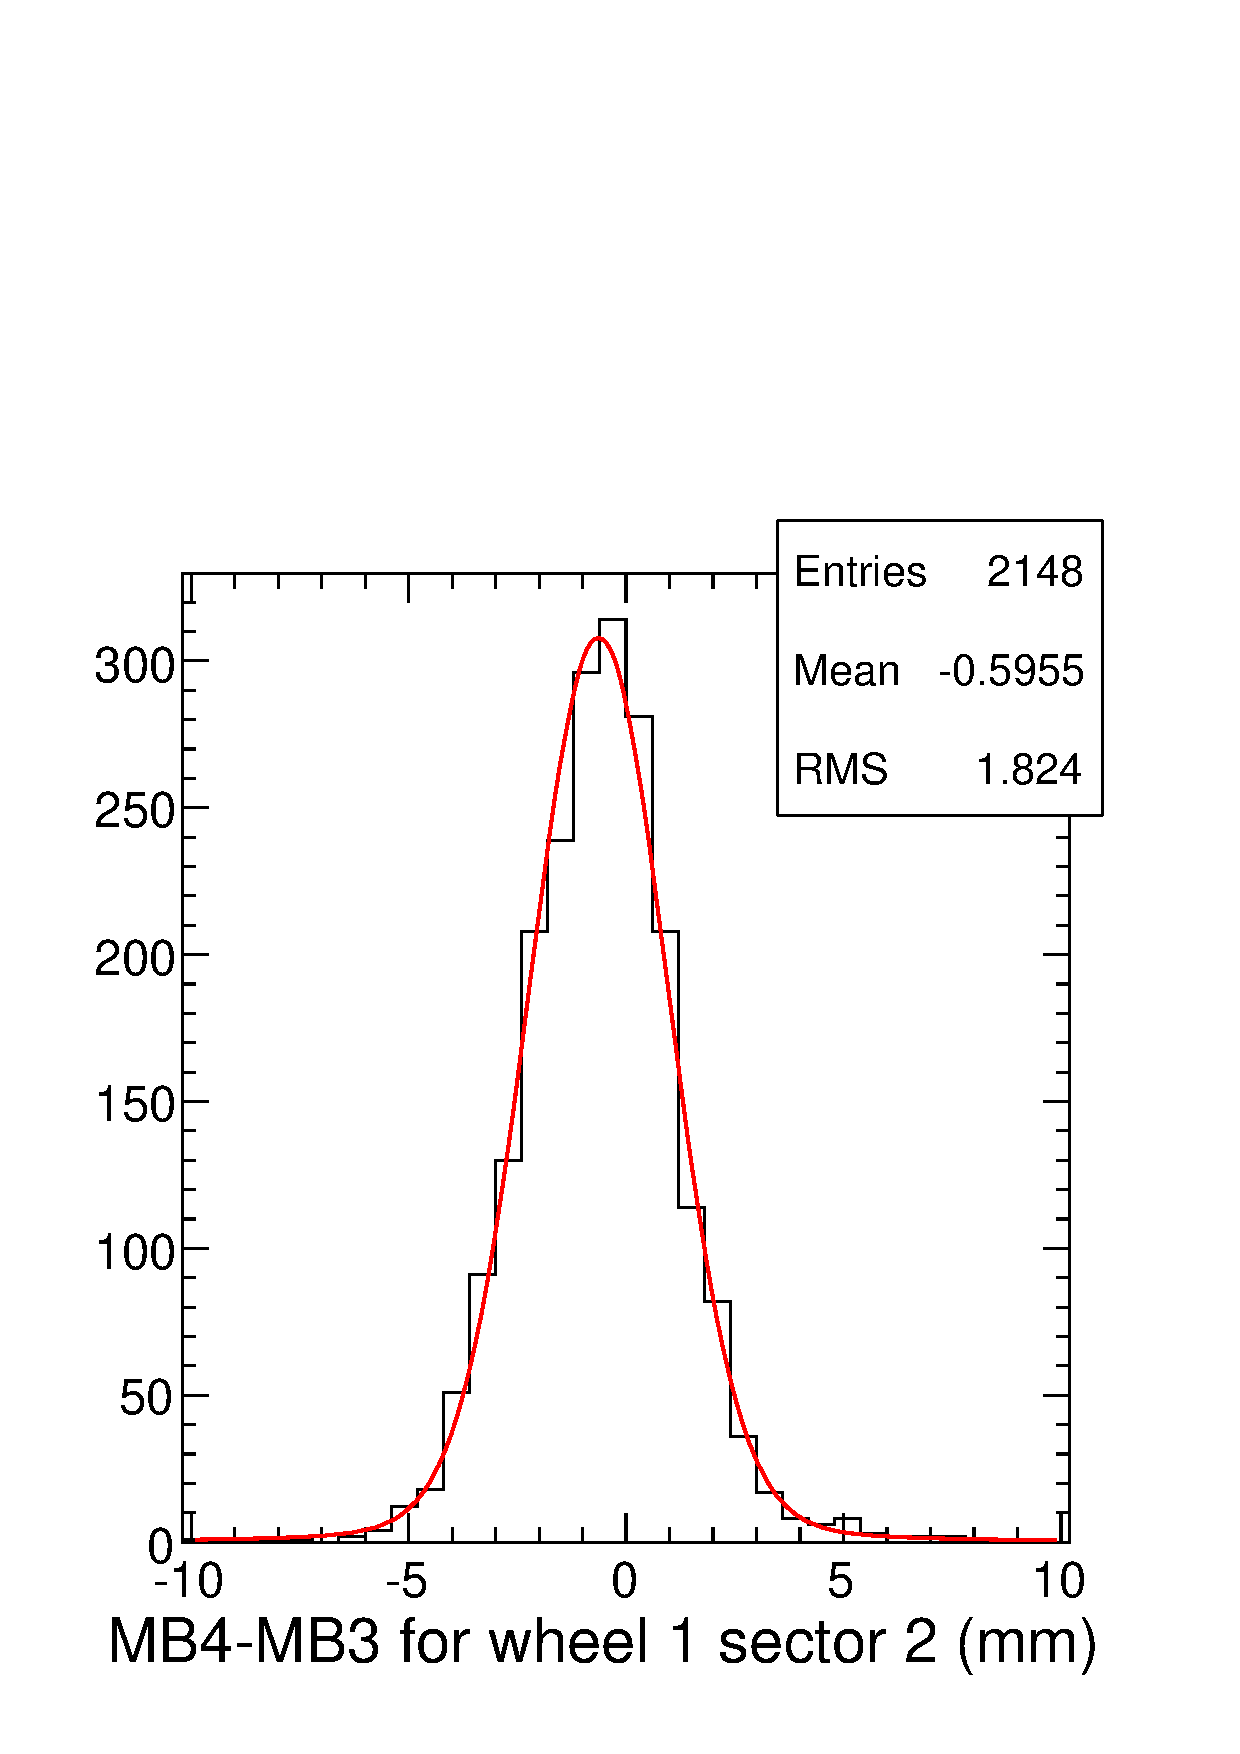
\includegraphics[width=0.25\linewidth]{diffindivx_1_34_2.pdf}
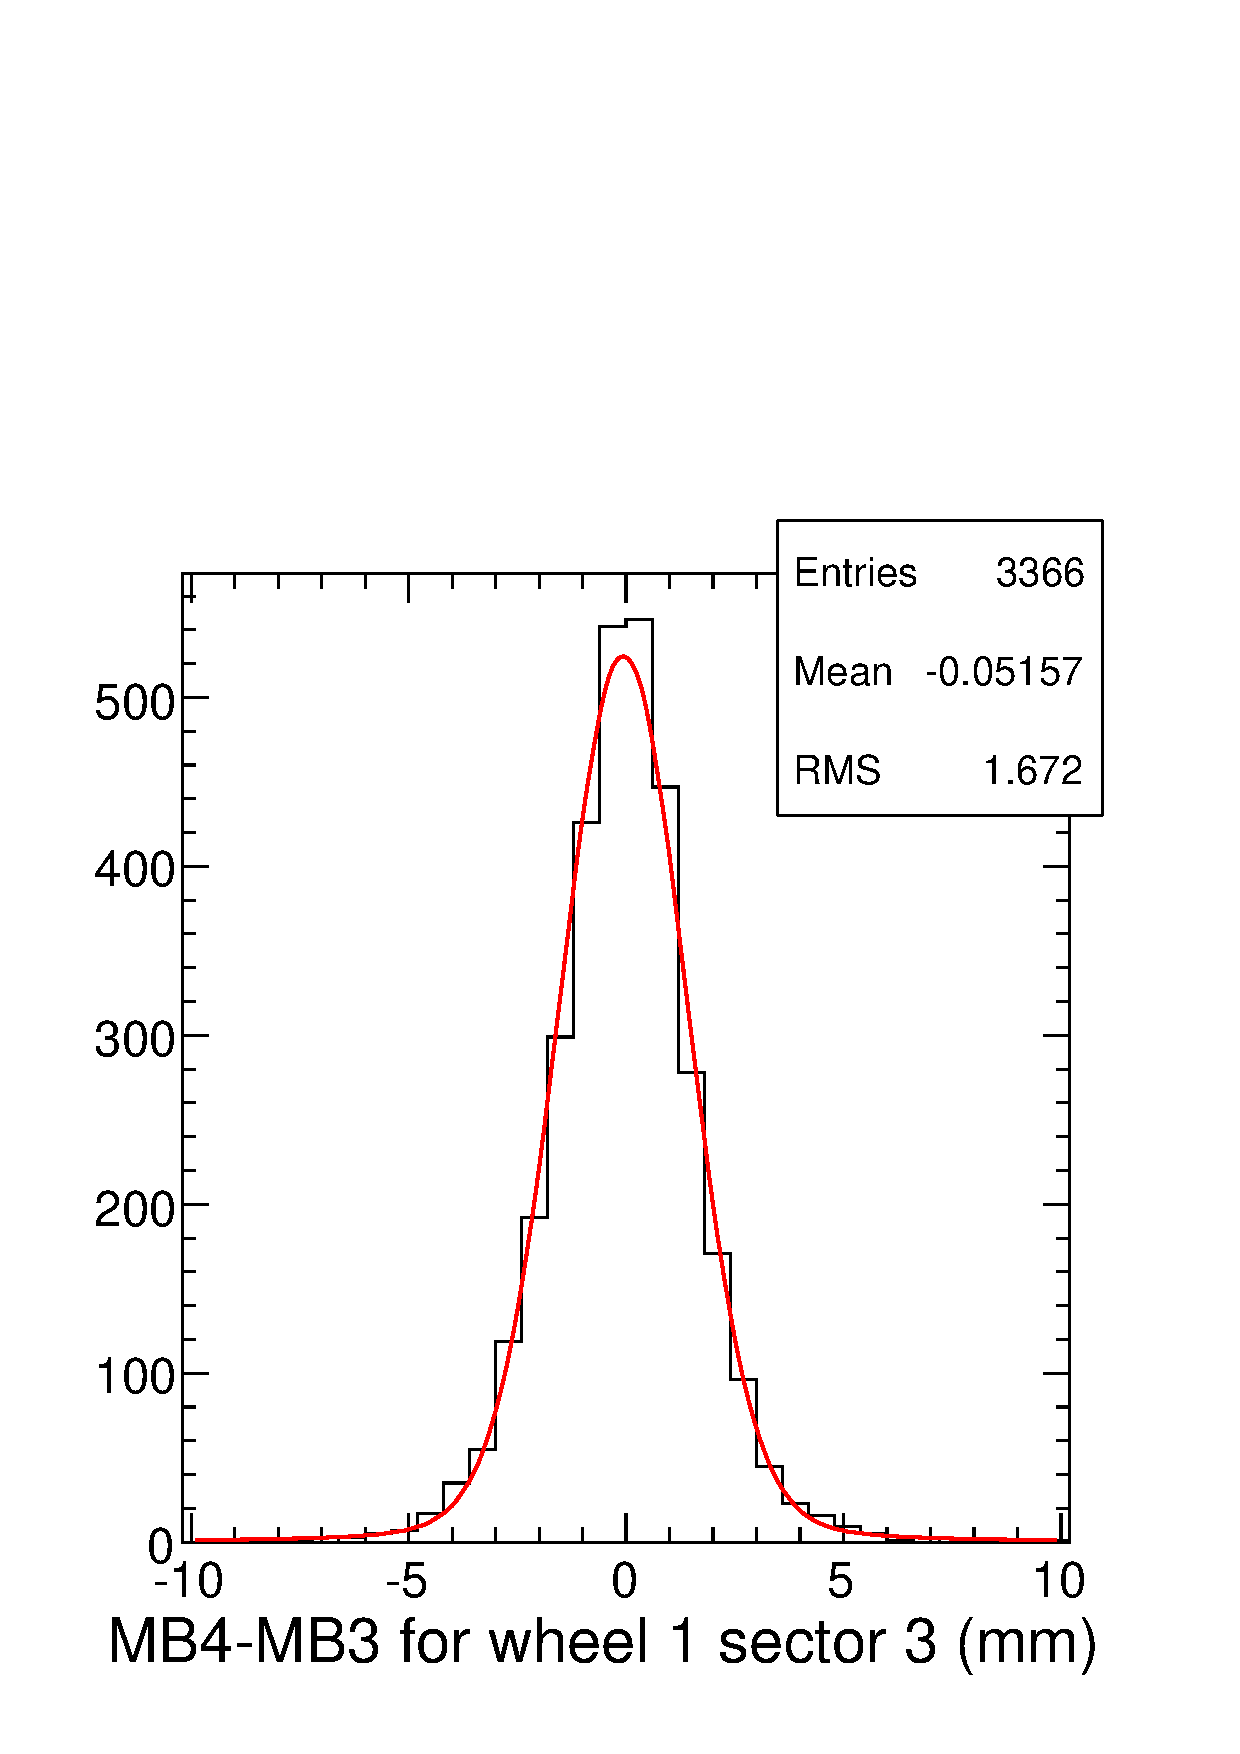
\includegraphics[width=0.25\linewidth]{diffindivx_1_34_3.pdf}
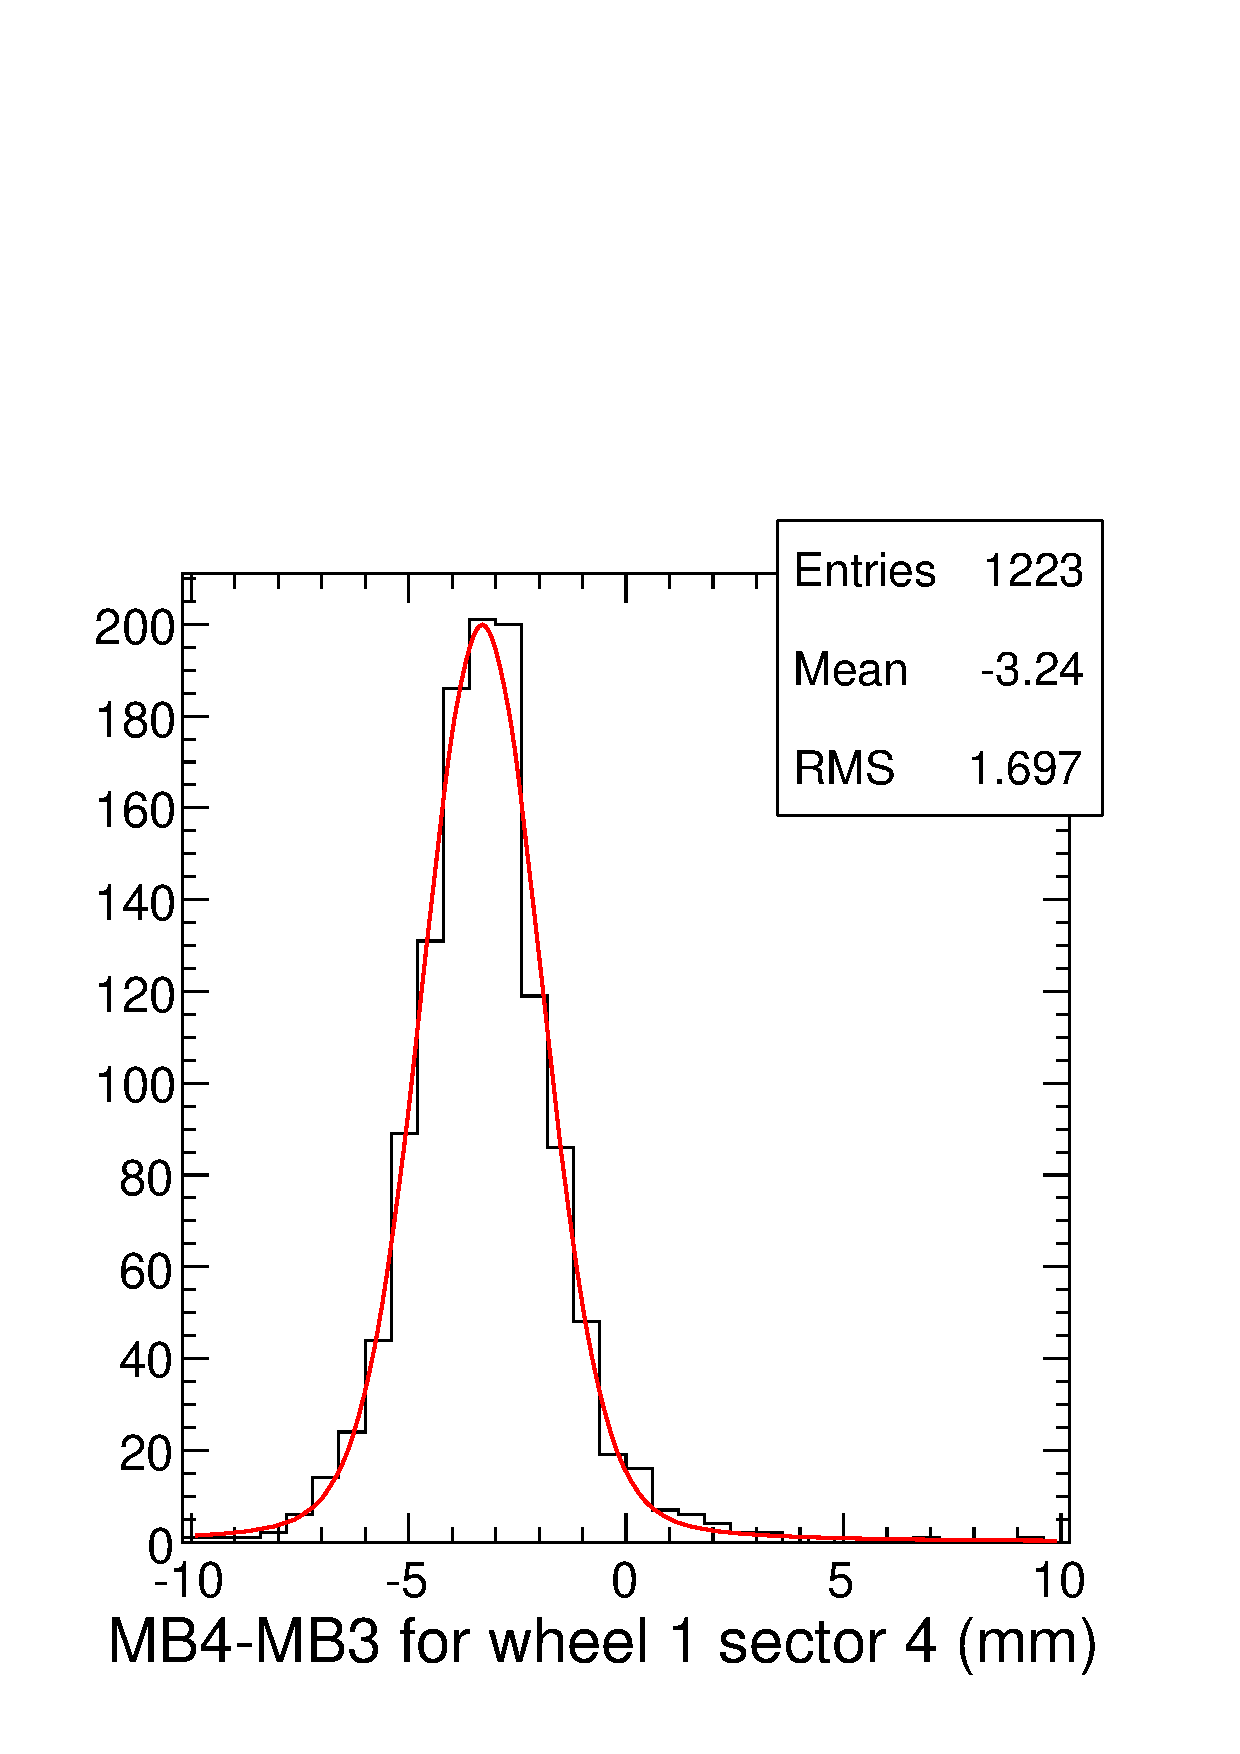
\includegraphics[width=0.25\linewidth]{diffindivx_1_34_4.pdf}

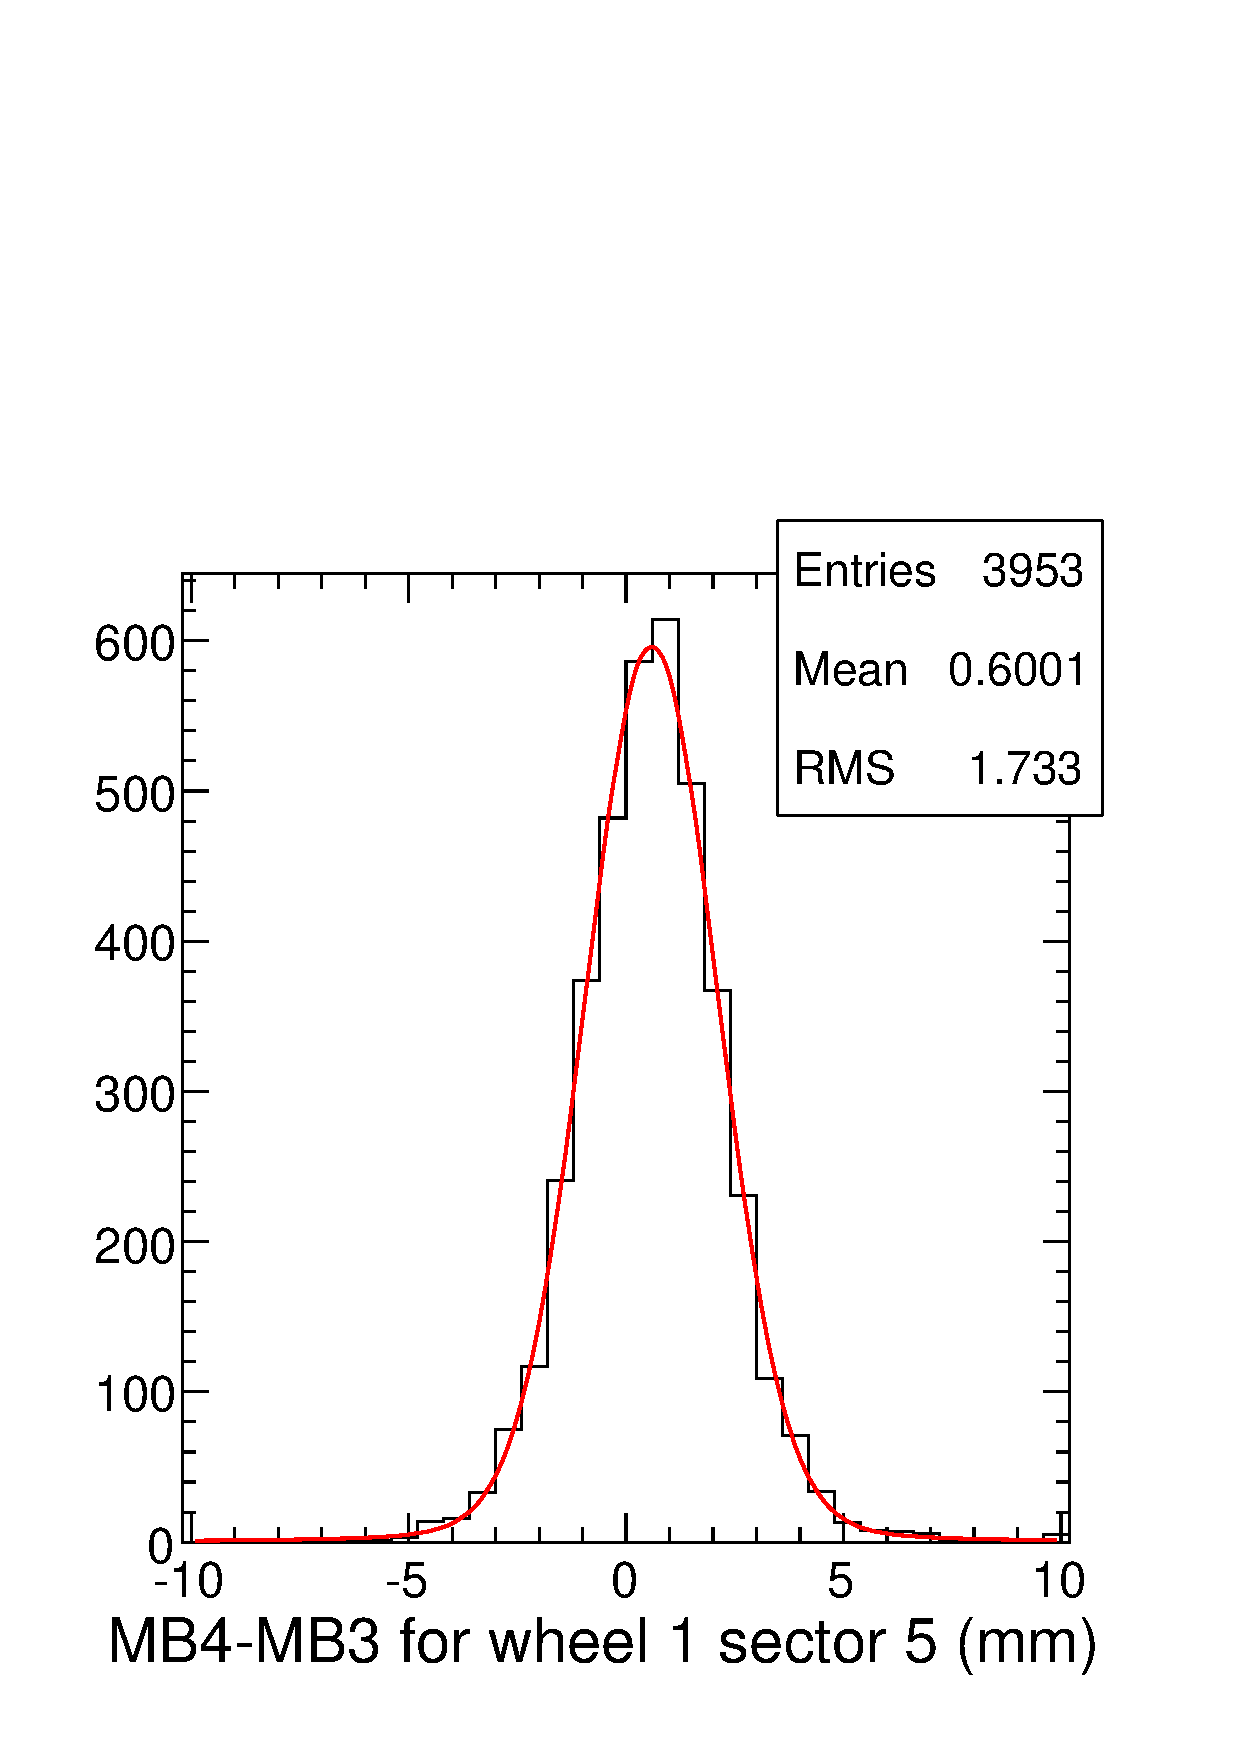
\includegraphics[width=0.25\linewidth]{diffindivx_1_34_5.pdf}
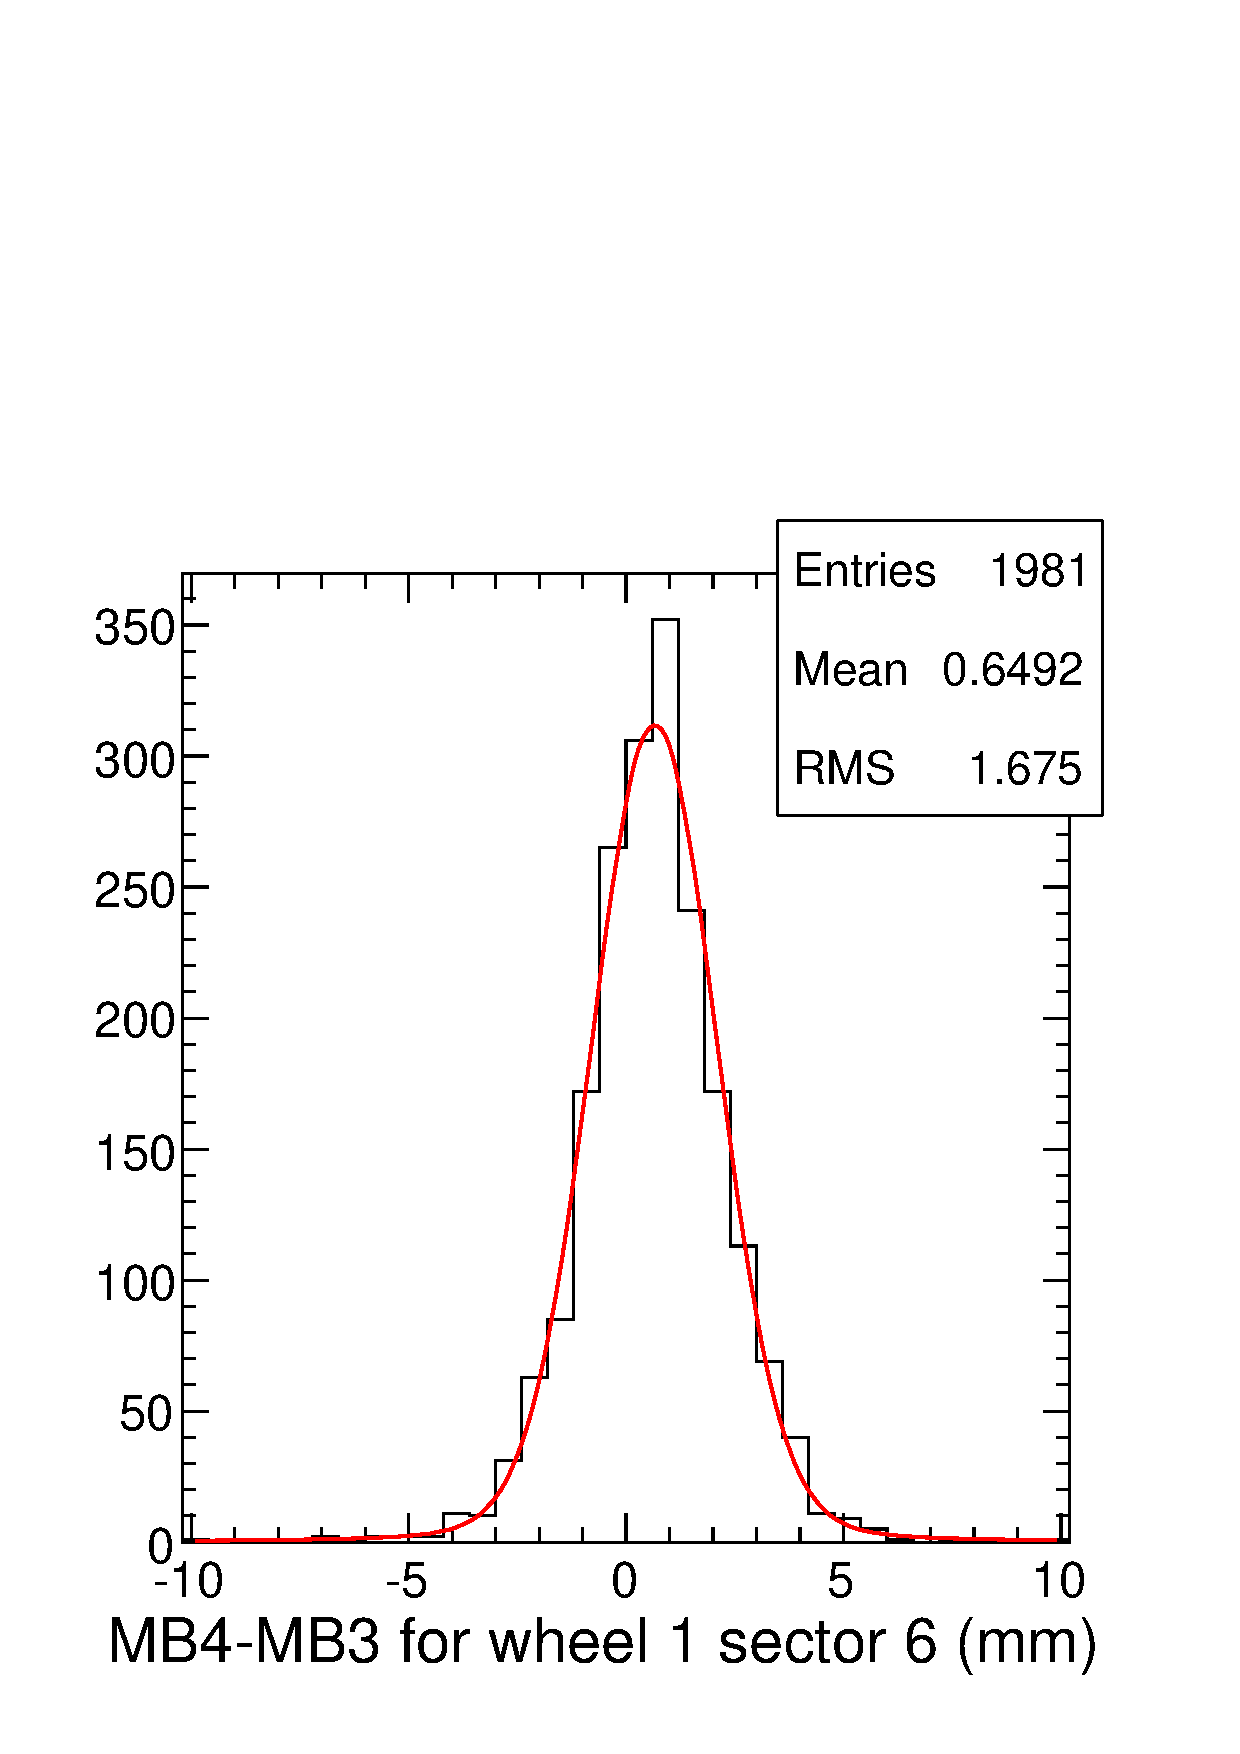
\includegraphics[width=0.25\linewidth]{diffindivx_1_34_6.pdf}
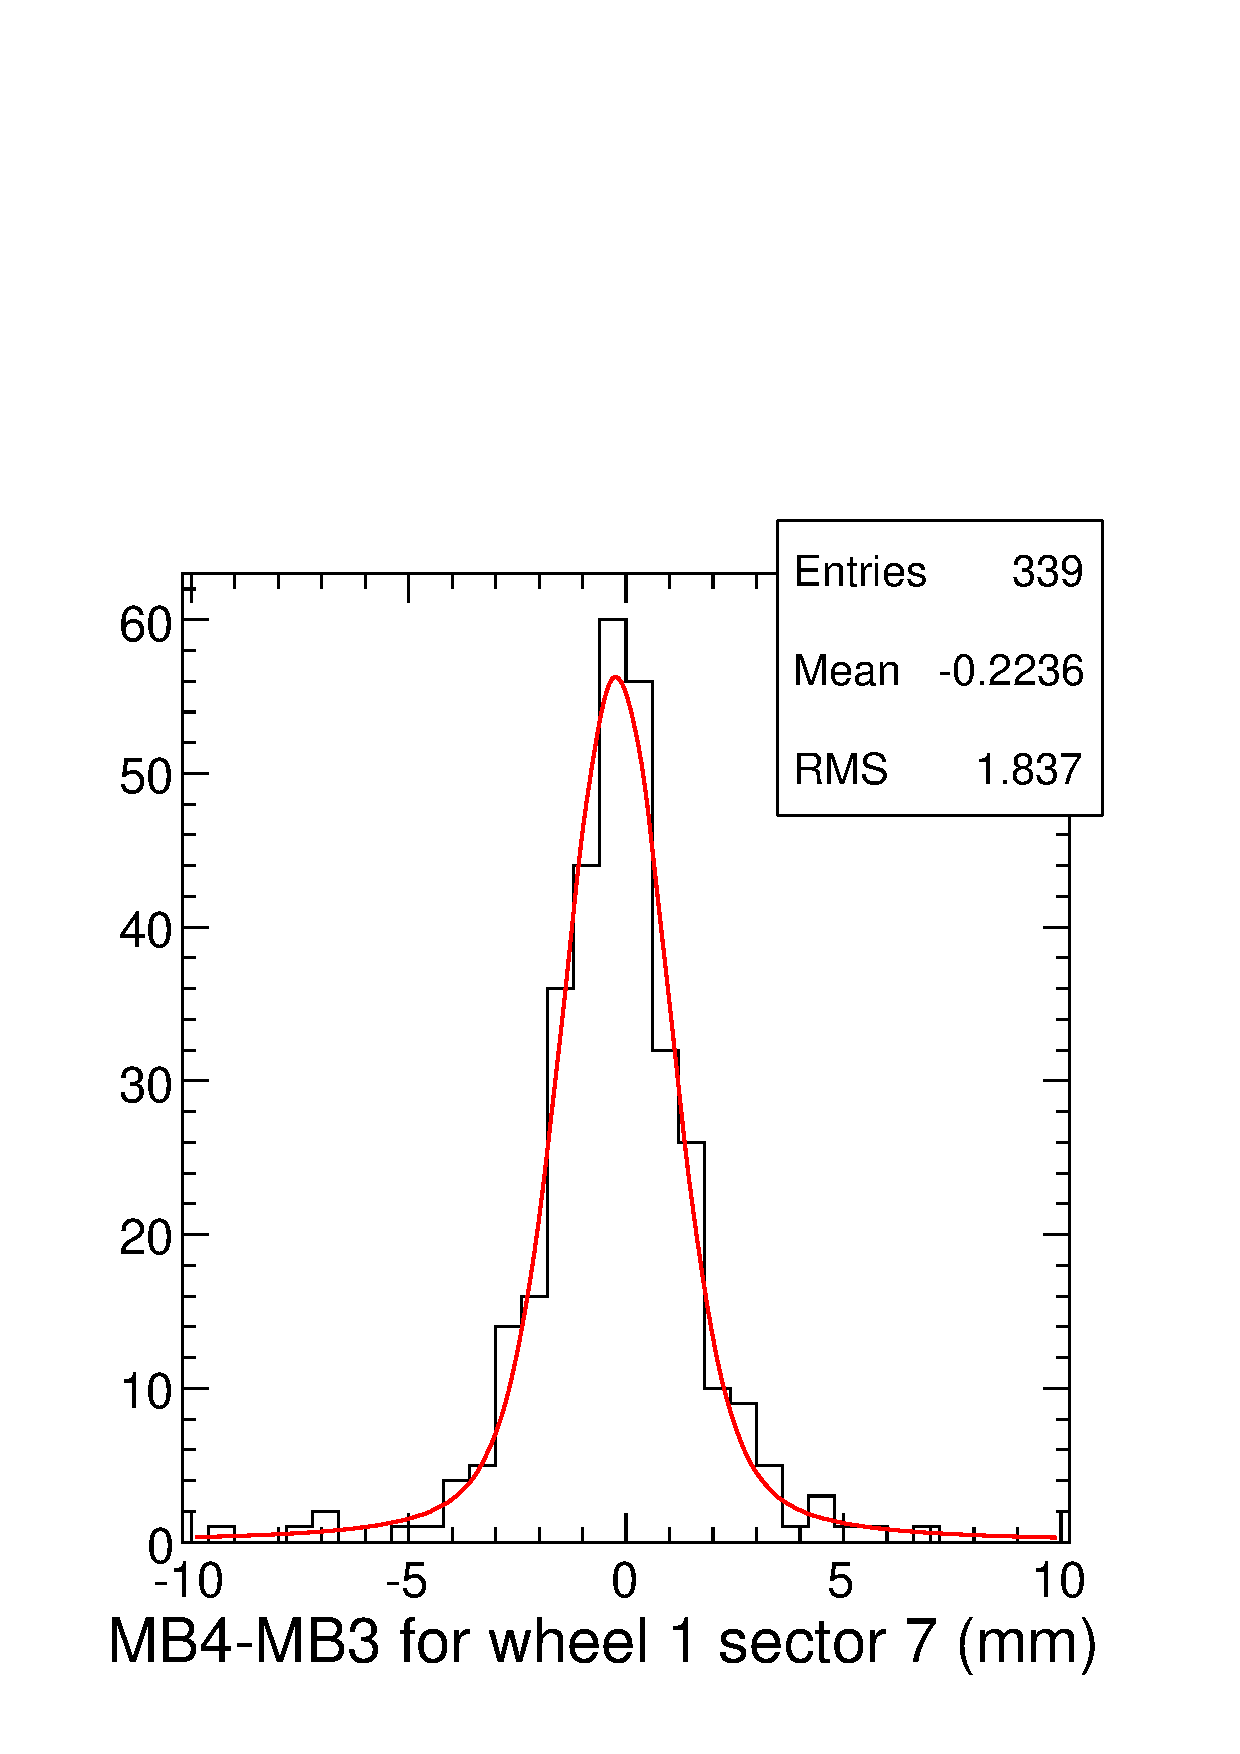
\includegraphics[width=0.25\linewidth]{diffindivx_1_34_7.pdf}
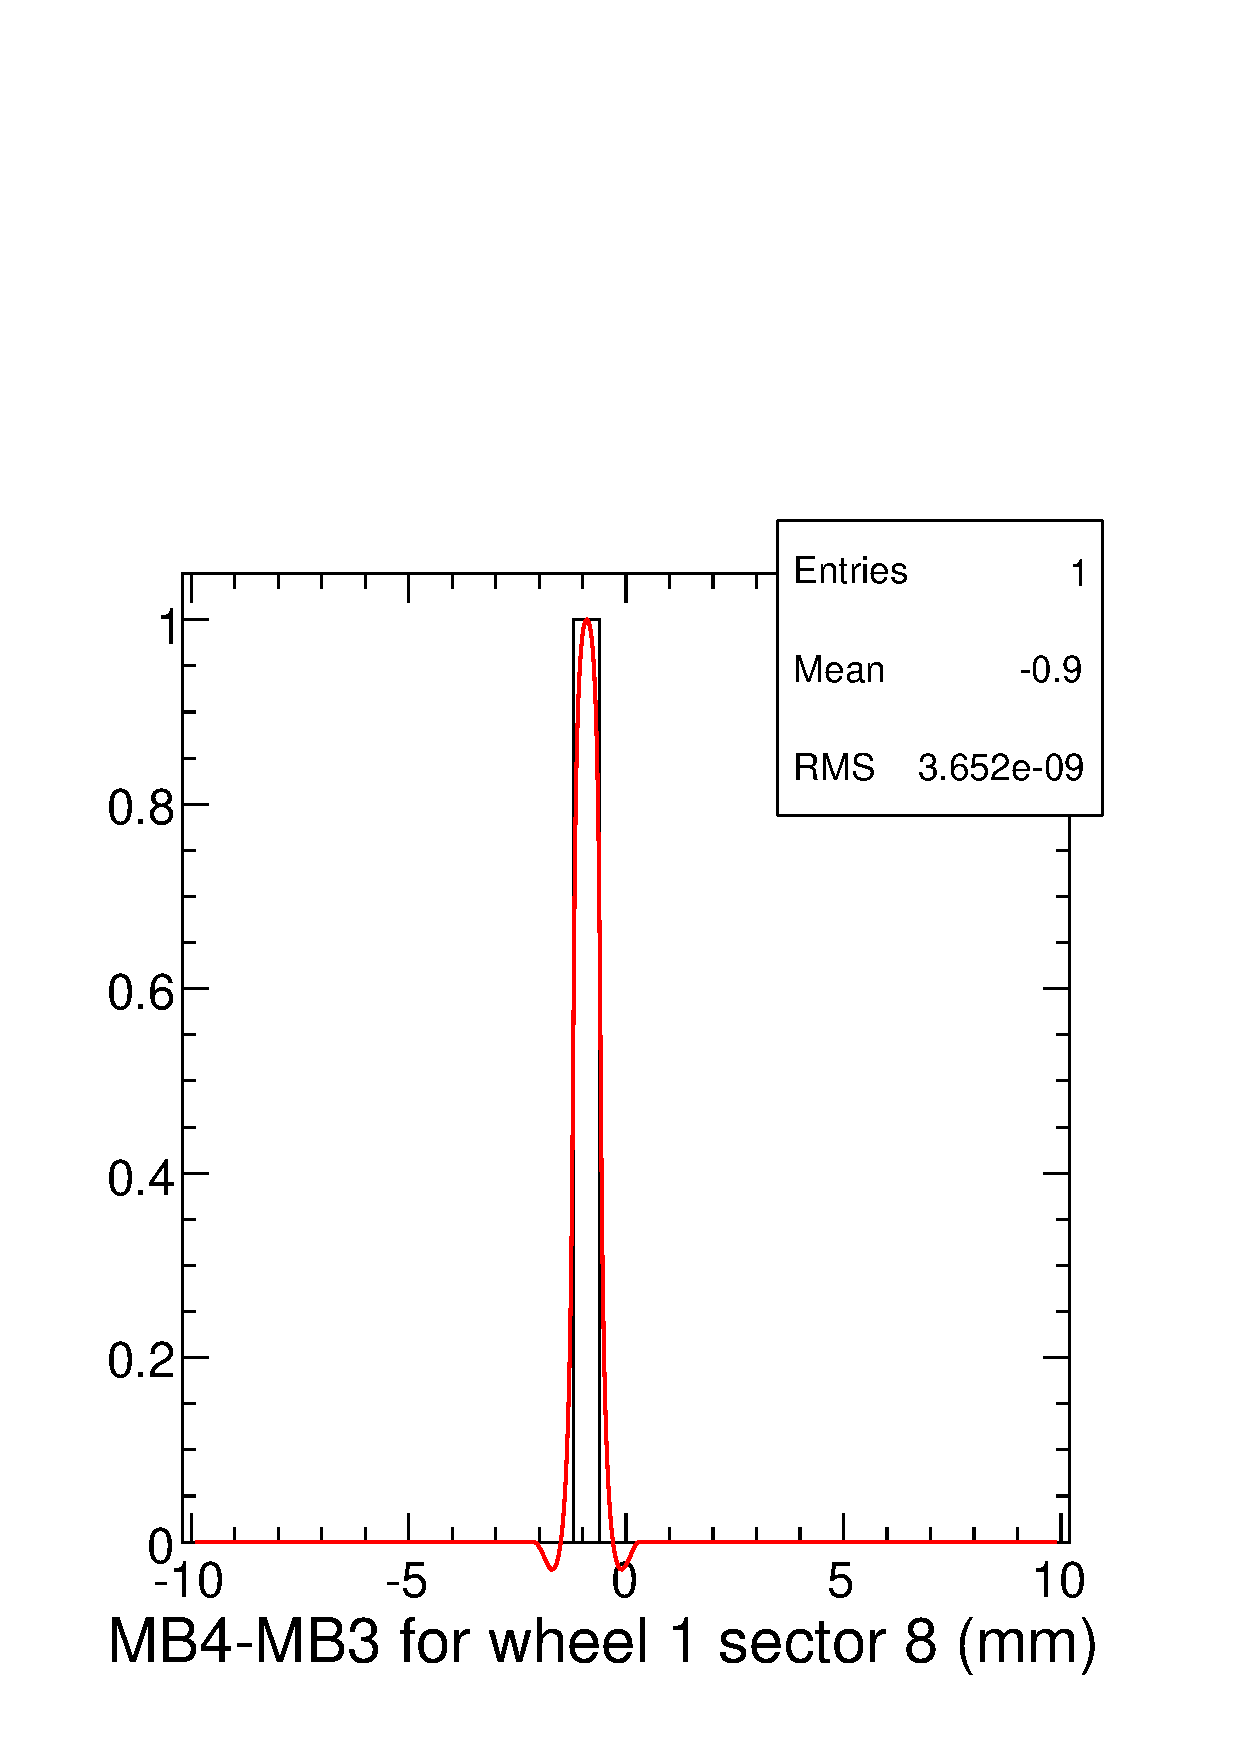
\includegraphics[width=0.25\linewidth]{diffindivx_1_34_8.pdf}

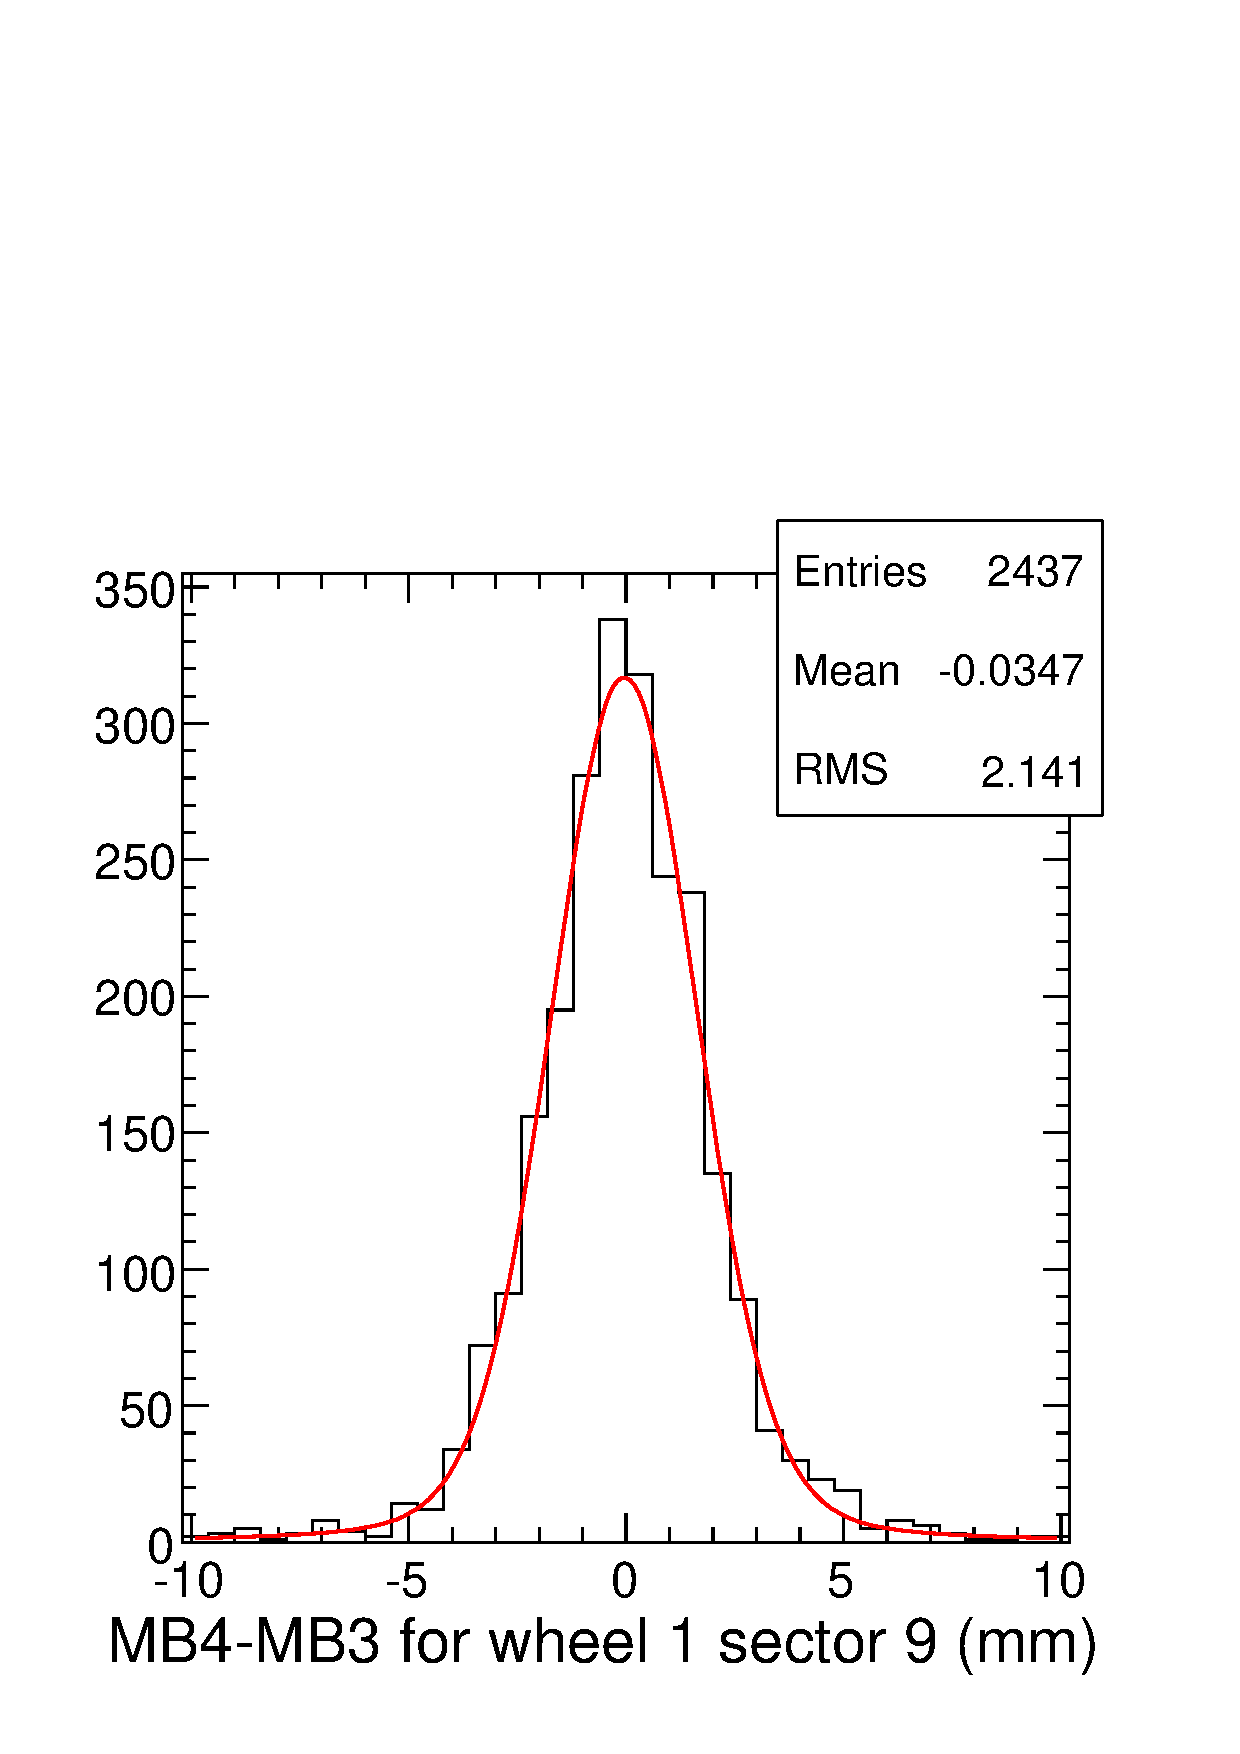
\includegraphics[width=0.25\linewidth]{diffindivx_1_34_9.pdf}
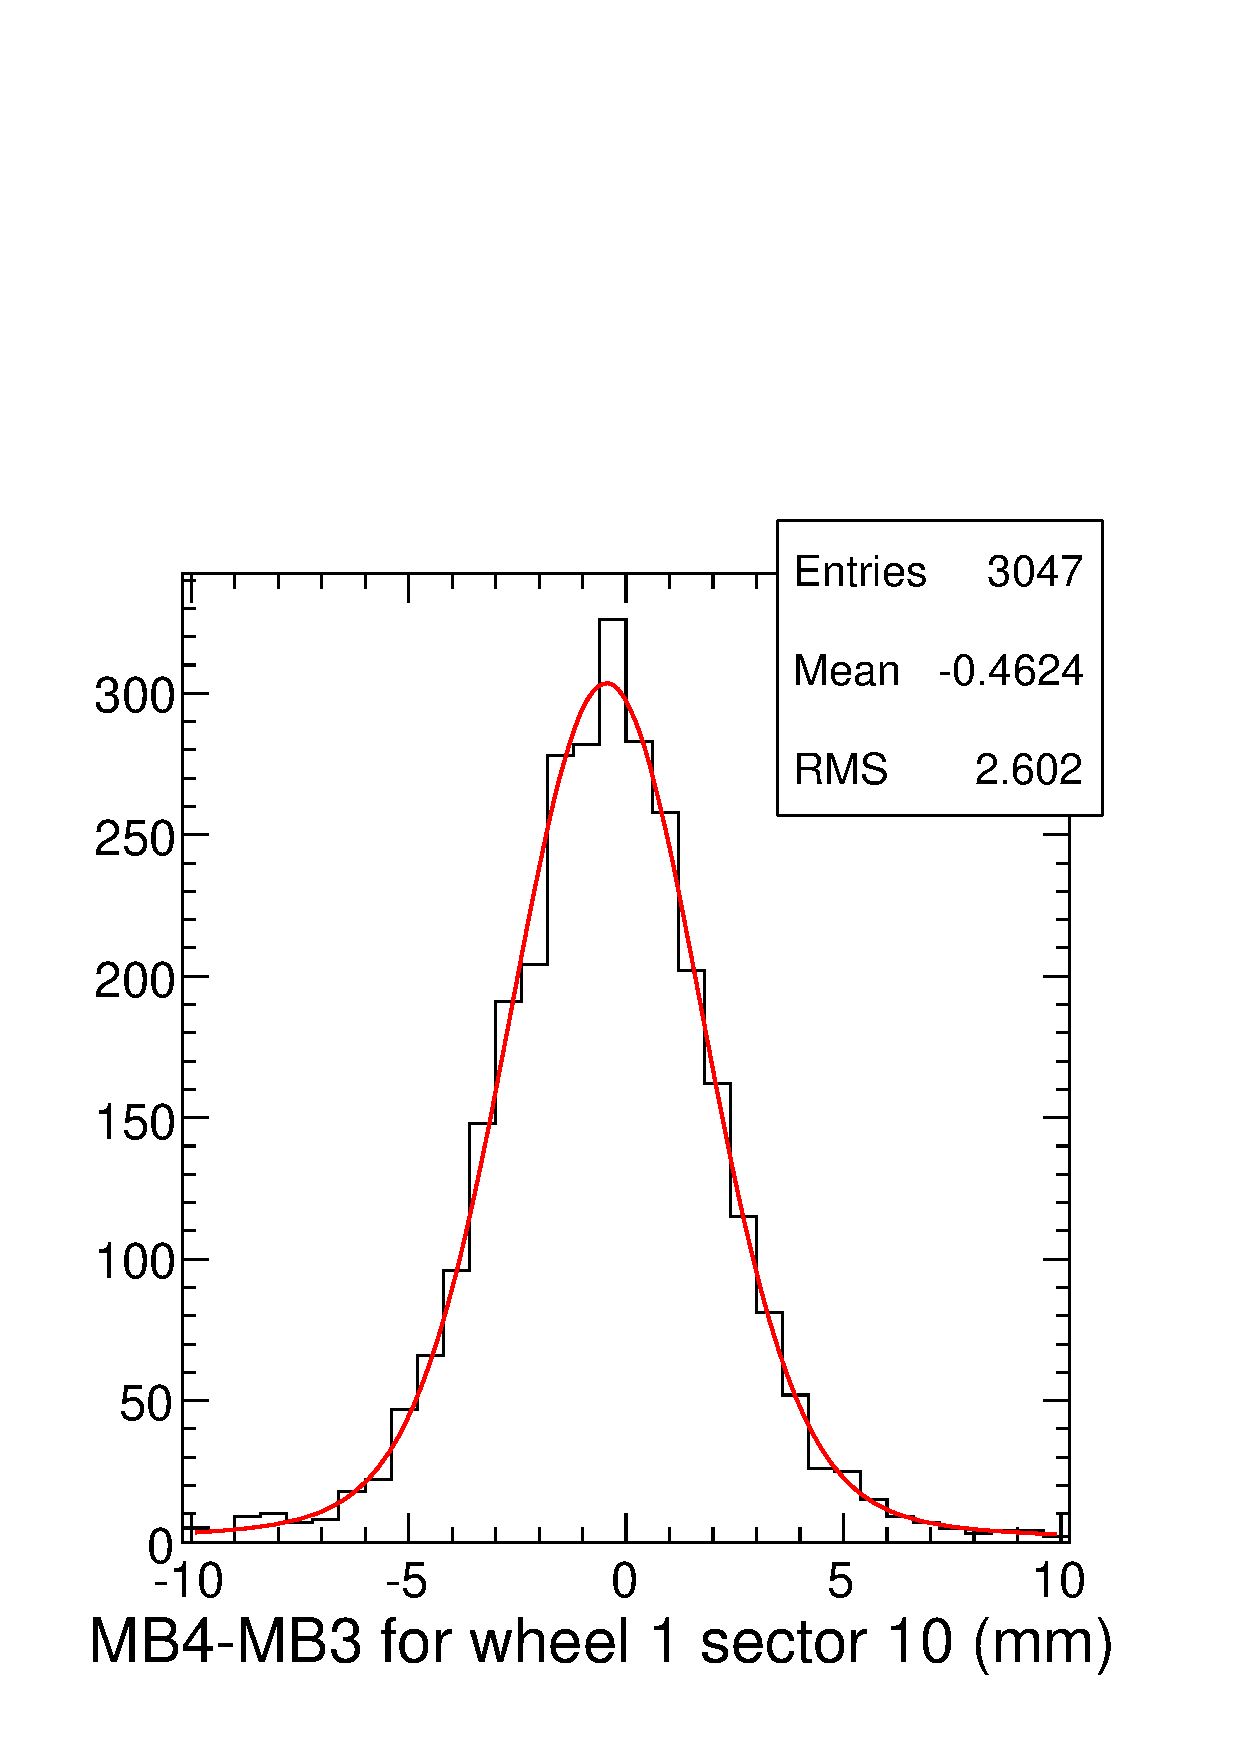
\includegraphics[width=0.25\linewidth]{diffindivx_1_34_10.pdf}
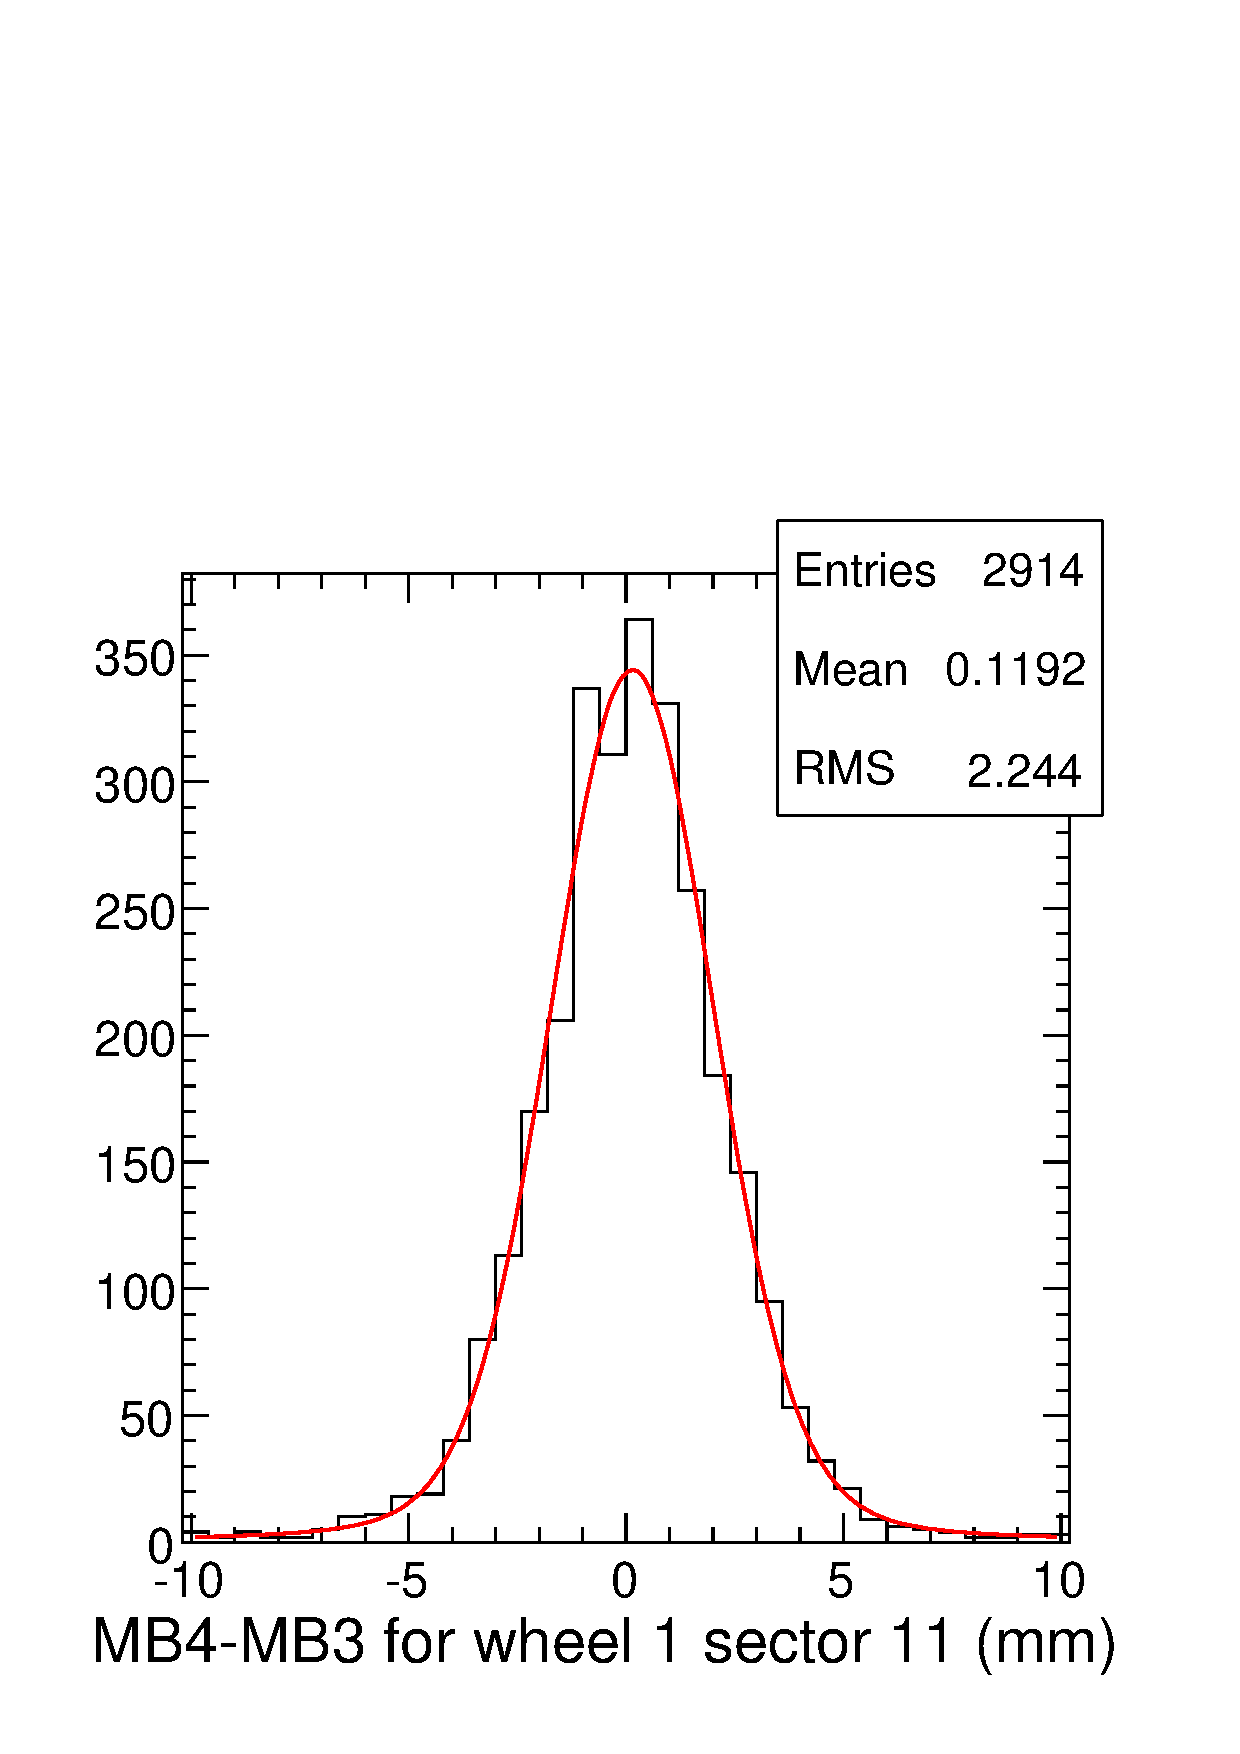
\includegraphics[width=0.25\linewidth]{diffindivx_1_34_11.pdf}
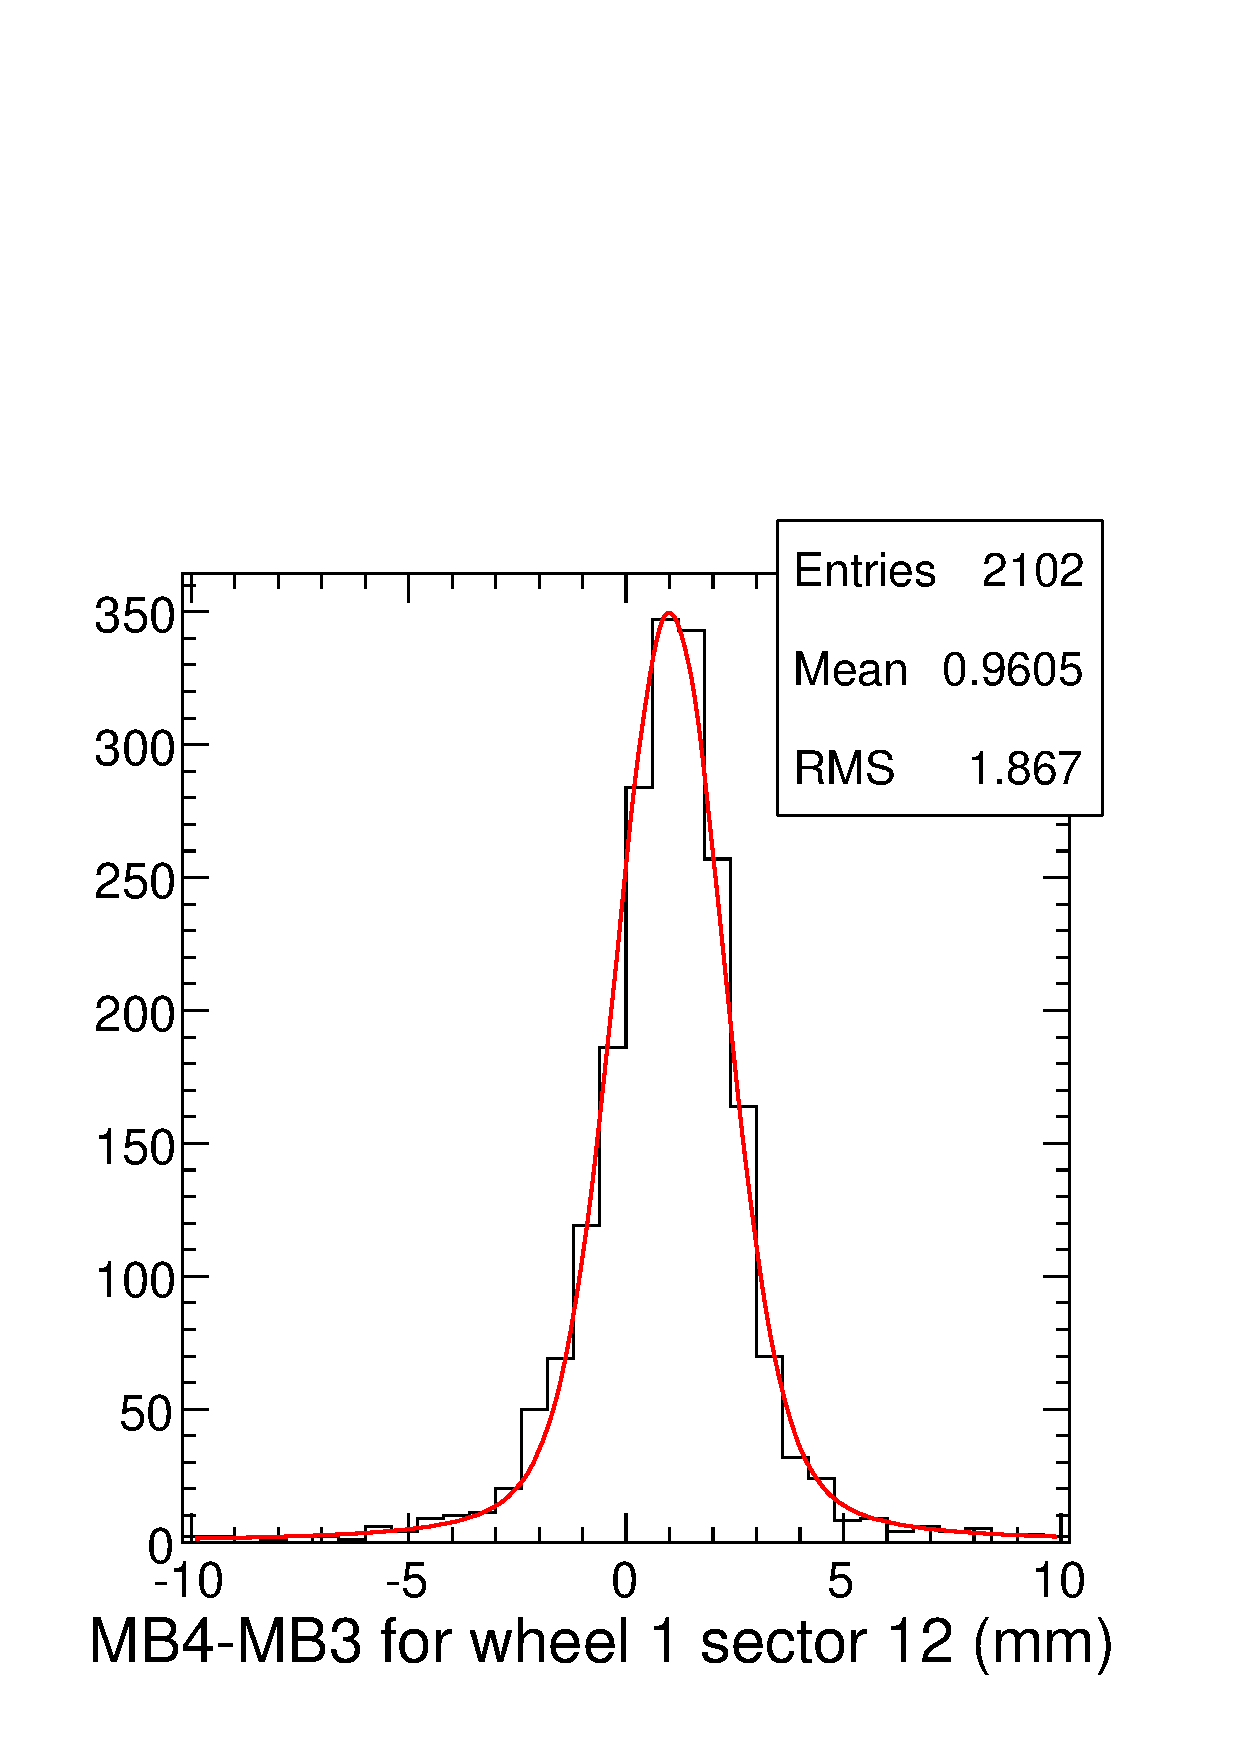
\includegraphics[width=0.25\linewidth]{diffindivx_1_34_12.pdf}

\column{0.3\linewidth}
\scriptsize Chambers with too few tracks for alignment, such as sector 8, are excluded from the plots on the following pages
\end{columns}
\end{frame}

\begin{frame}
\frametitle{Differences by sector: $\phi_y$}
\begin{itemize}
\item Differences between stations 3 and 4 in wheel 1
\item Distributions have tails: fit with Gaussian $\otimes$ Lorentzian
\begin{itemize}
\item doesn't matter: fit result (circles, next pages) are nearly equal to the mean (stars), usually overlapping
\end{itemize}
\end{itemize}

\begin{columns}
\column{0.7\linewidth}
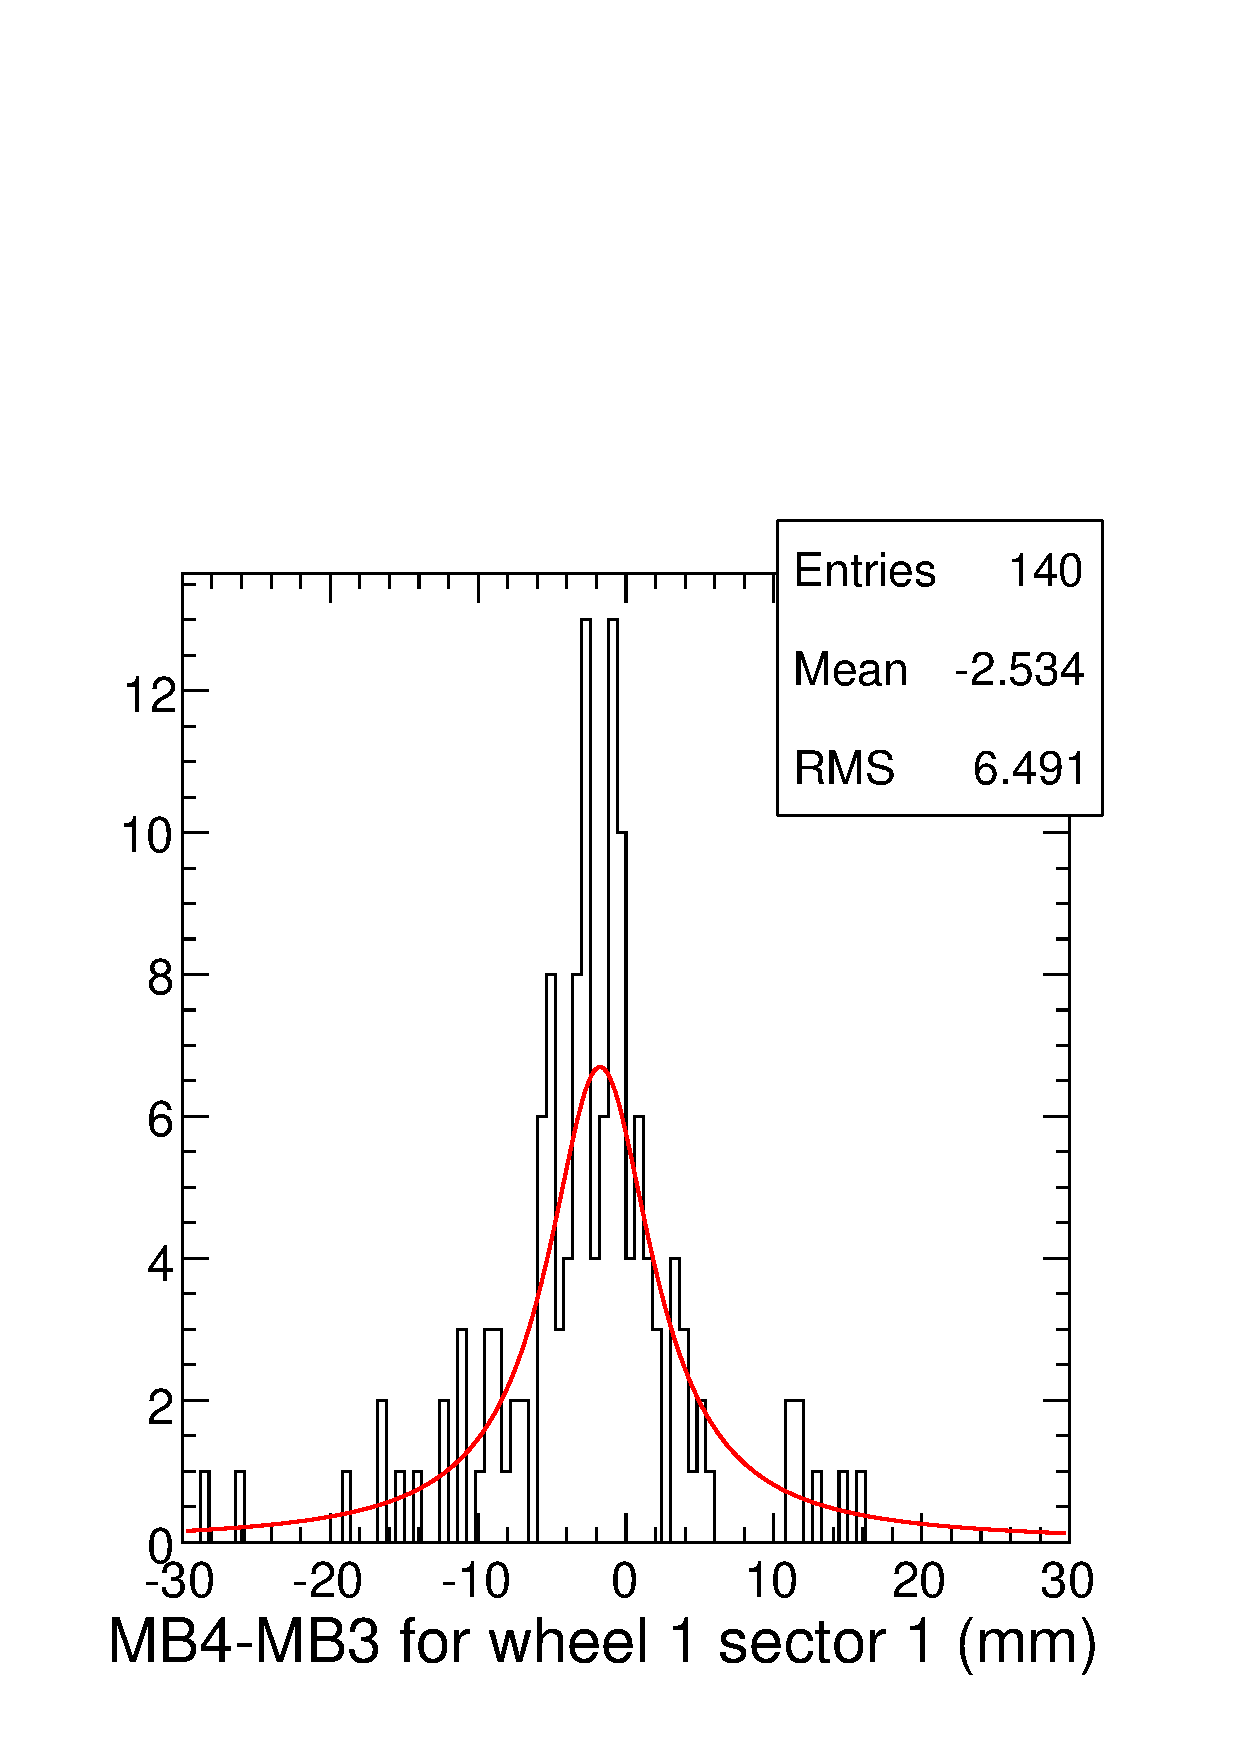
\includegraphics[width=0.25\linewidth]{diffindivphi_1_34_1.pdf}
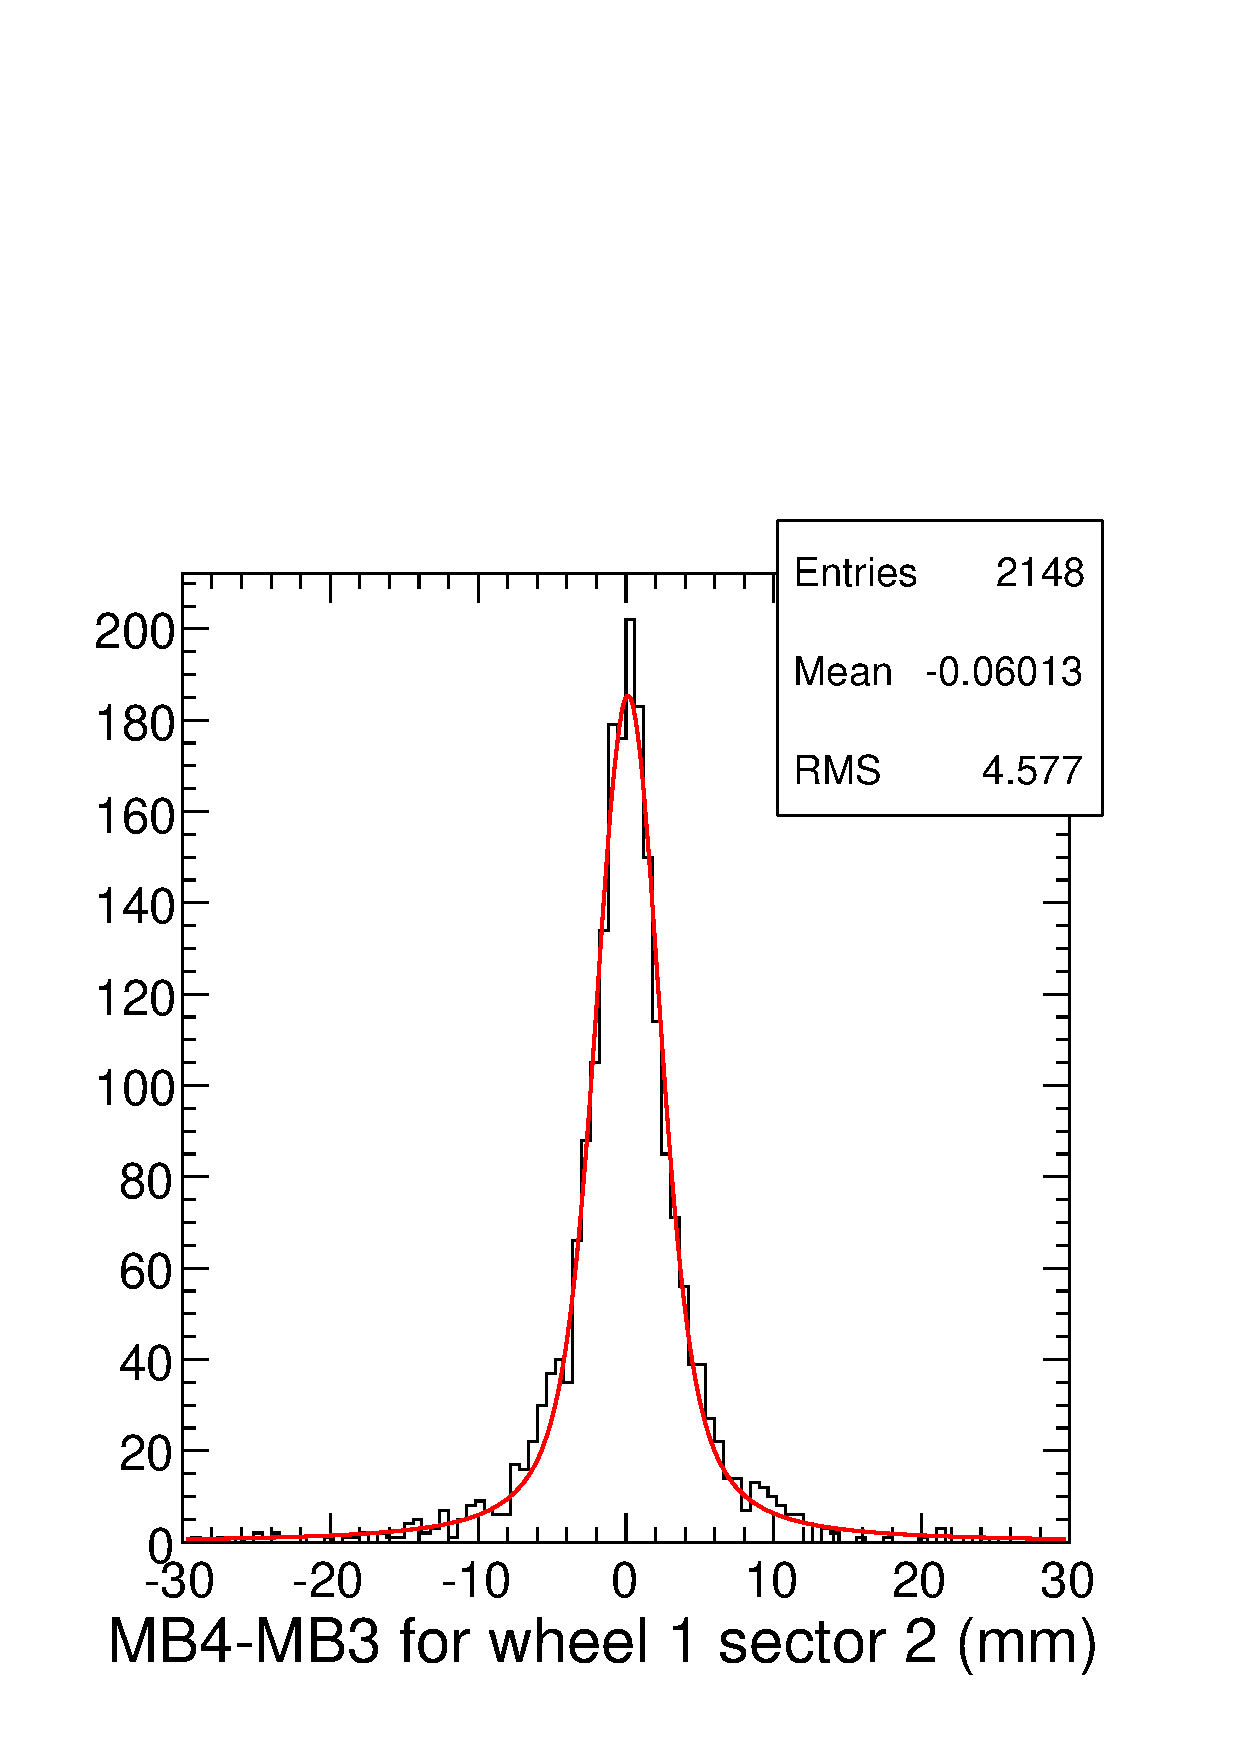
\includegraphics[width=0.25\linewidth]{diffindivphi_1_34_2.pdf}
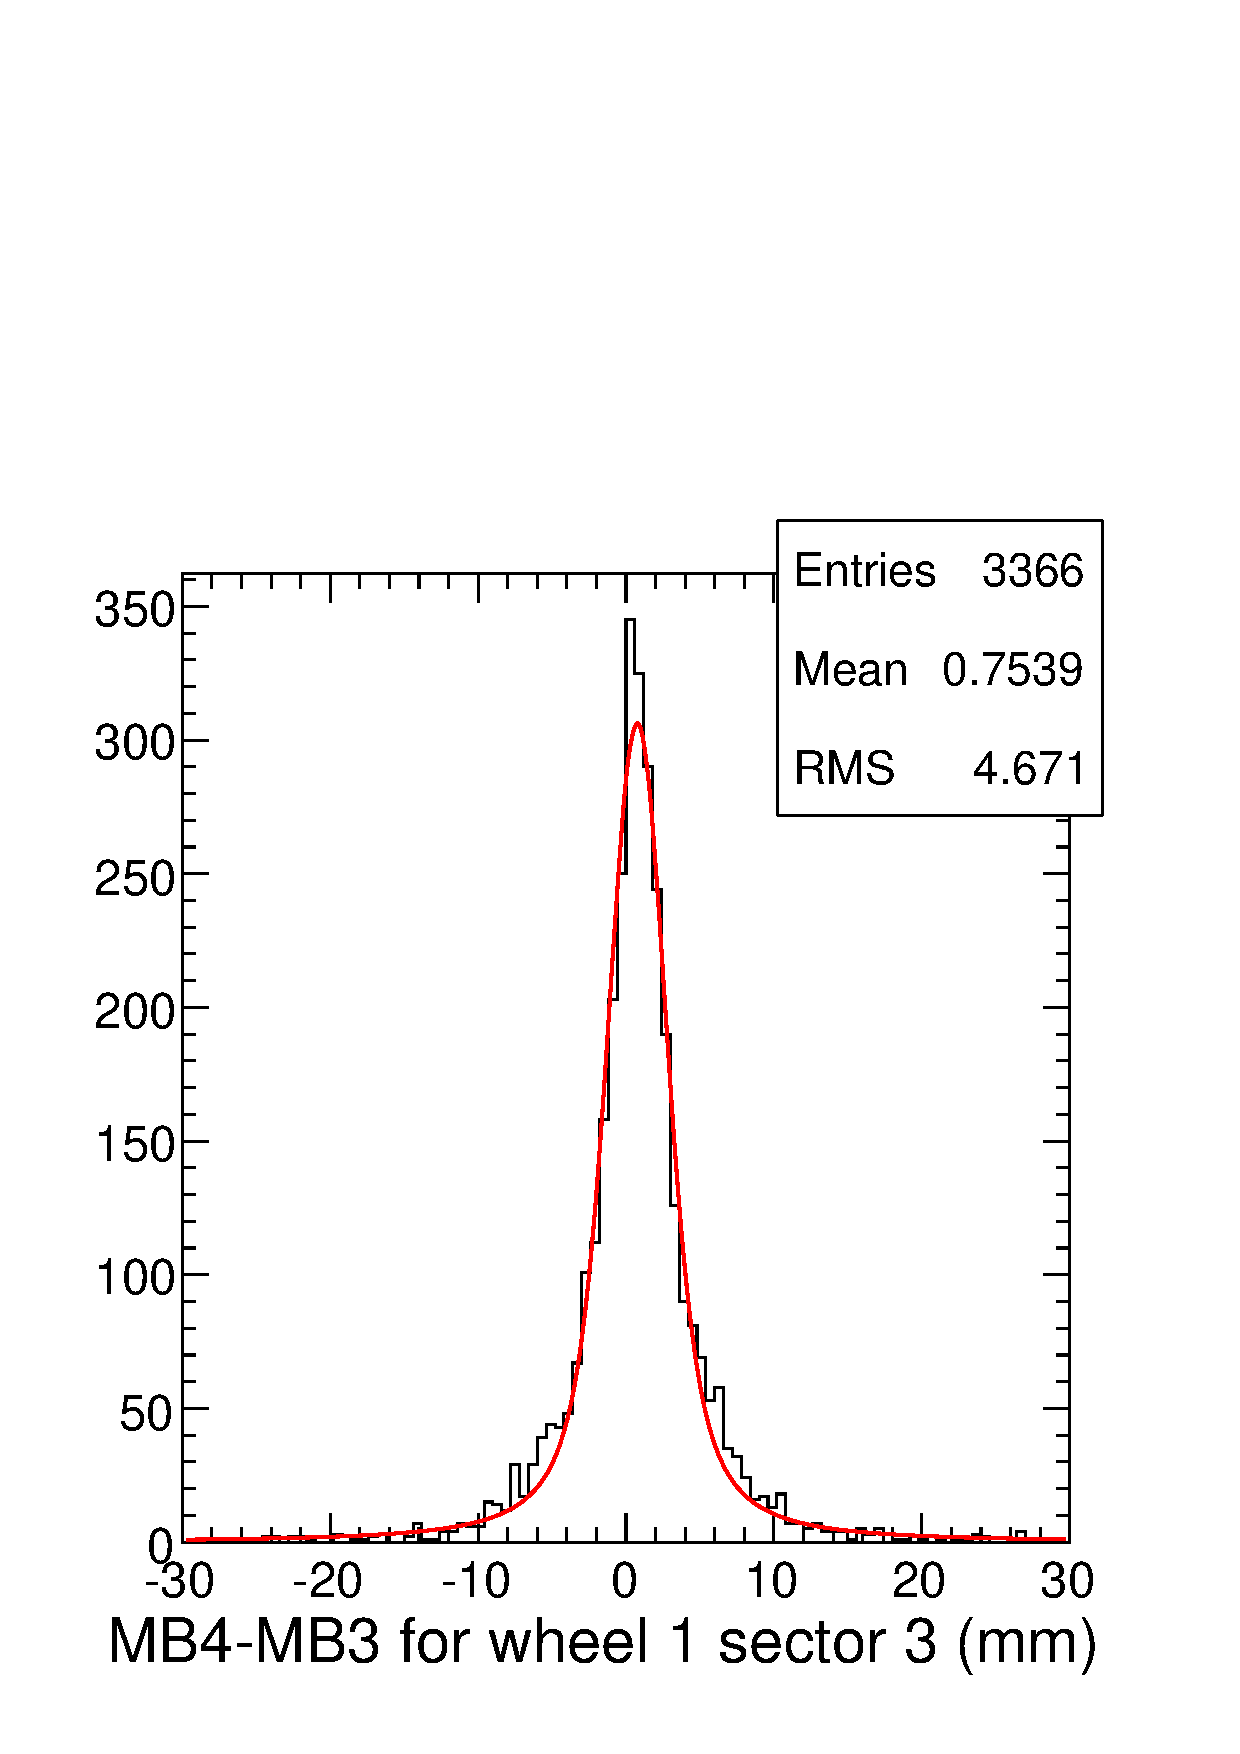
\includegraphics[width=0.25\linewidth]{diffindivphi_1_34_3.pdf}
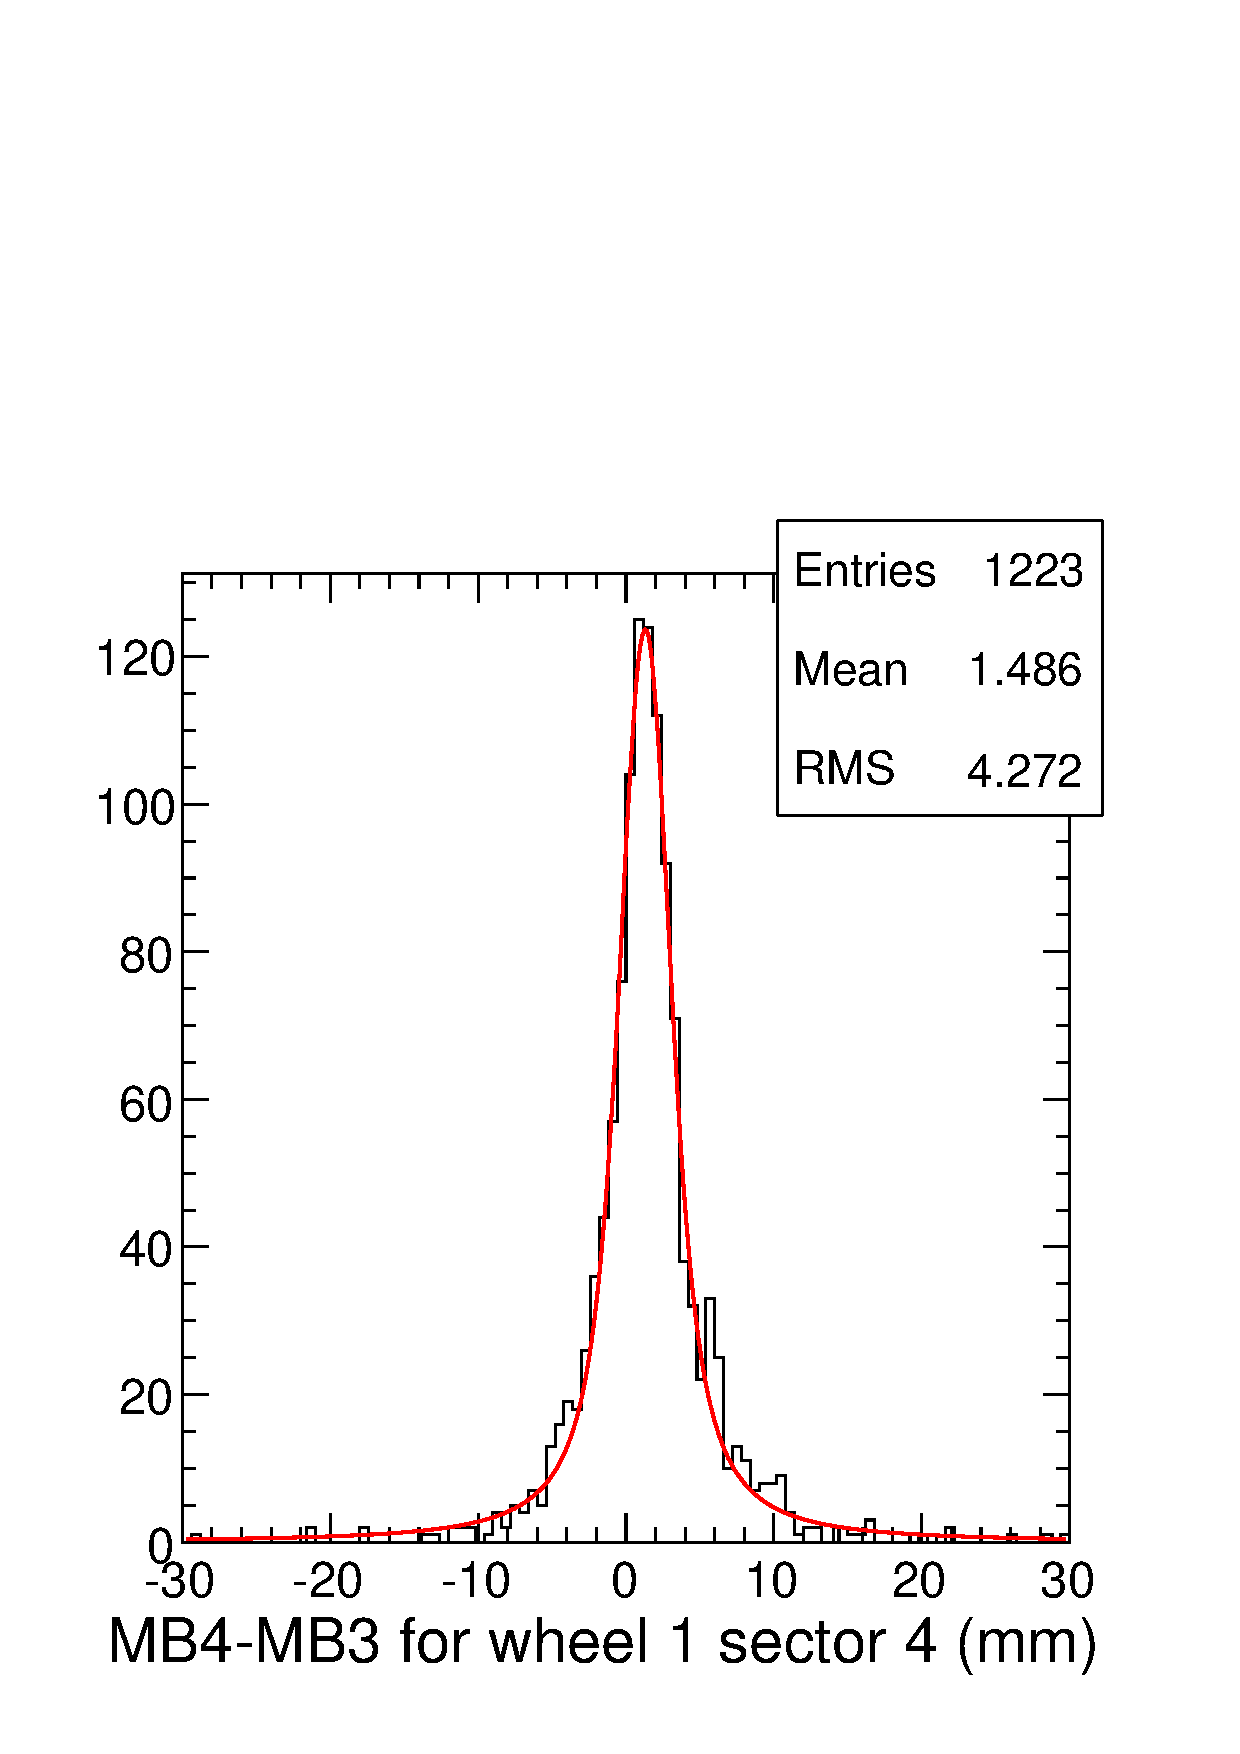
\includegraphics[width=0.25\linewidth]{diffindivphi_1_34_4.pdf}

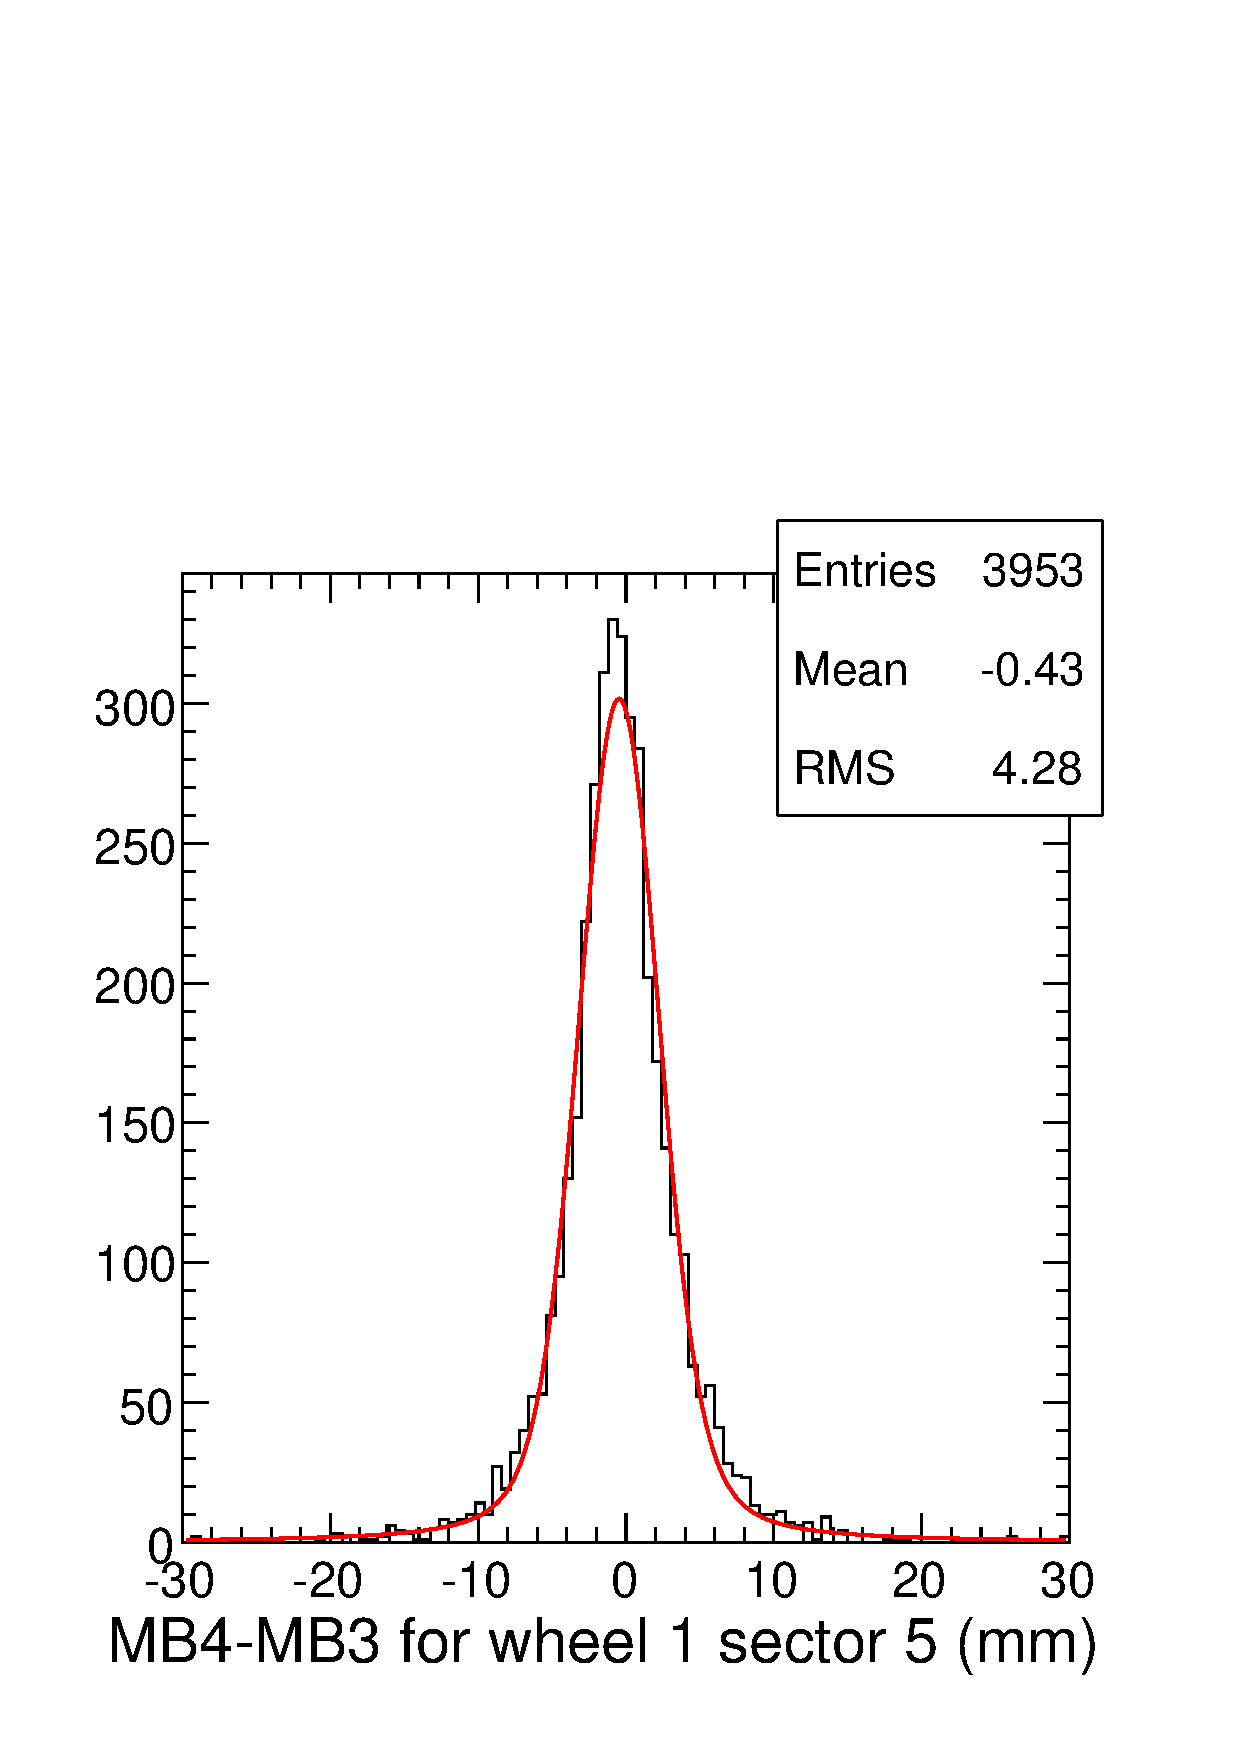
\includegraphics[width=0.25\linewidth]{diffindivphi_1_34_5.pdf}
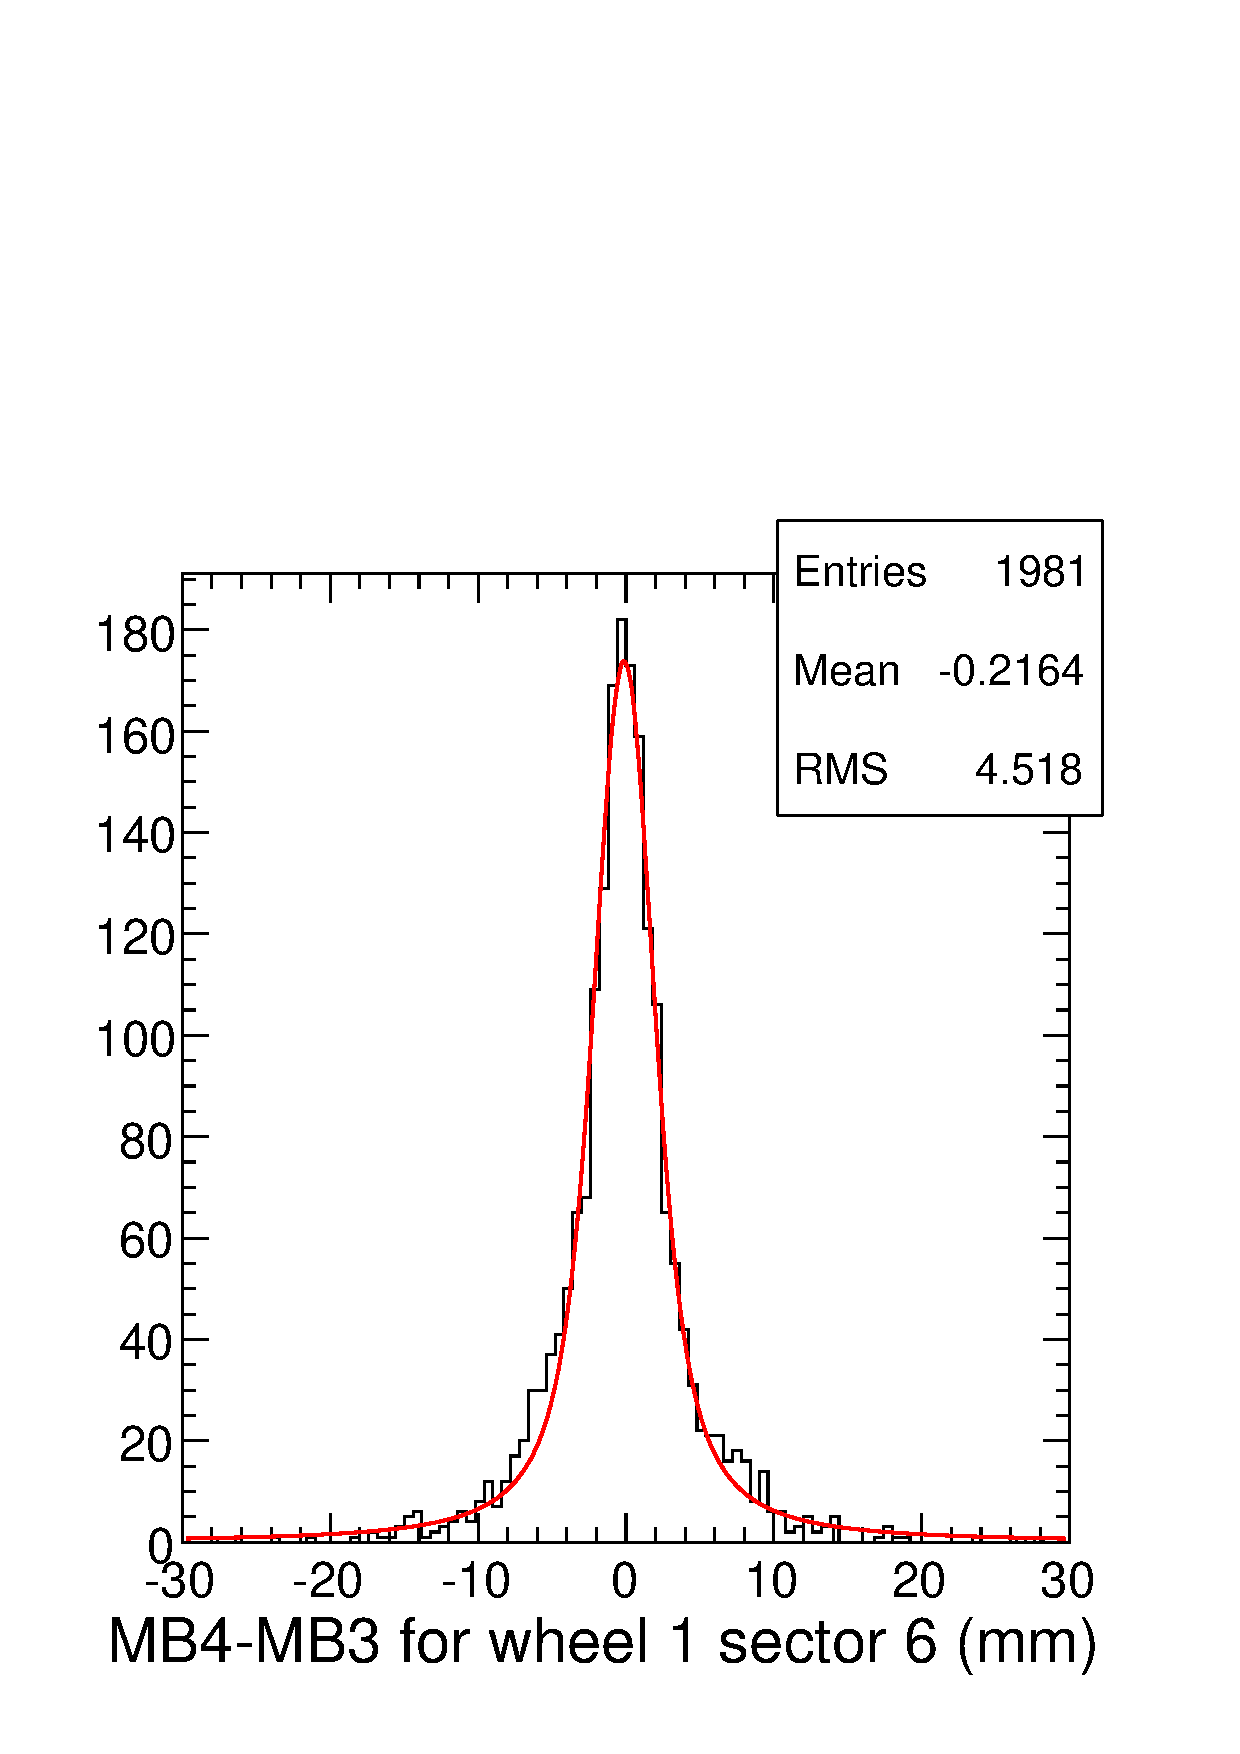
\includegraphics[width=0.25\linewidth]{diffindivphi_1_34_6.pdf}
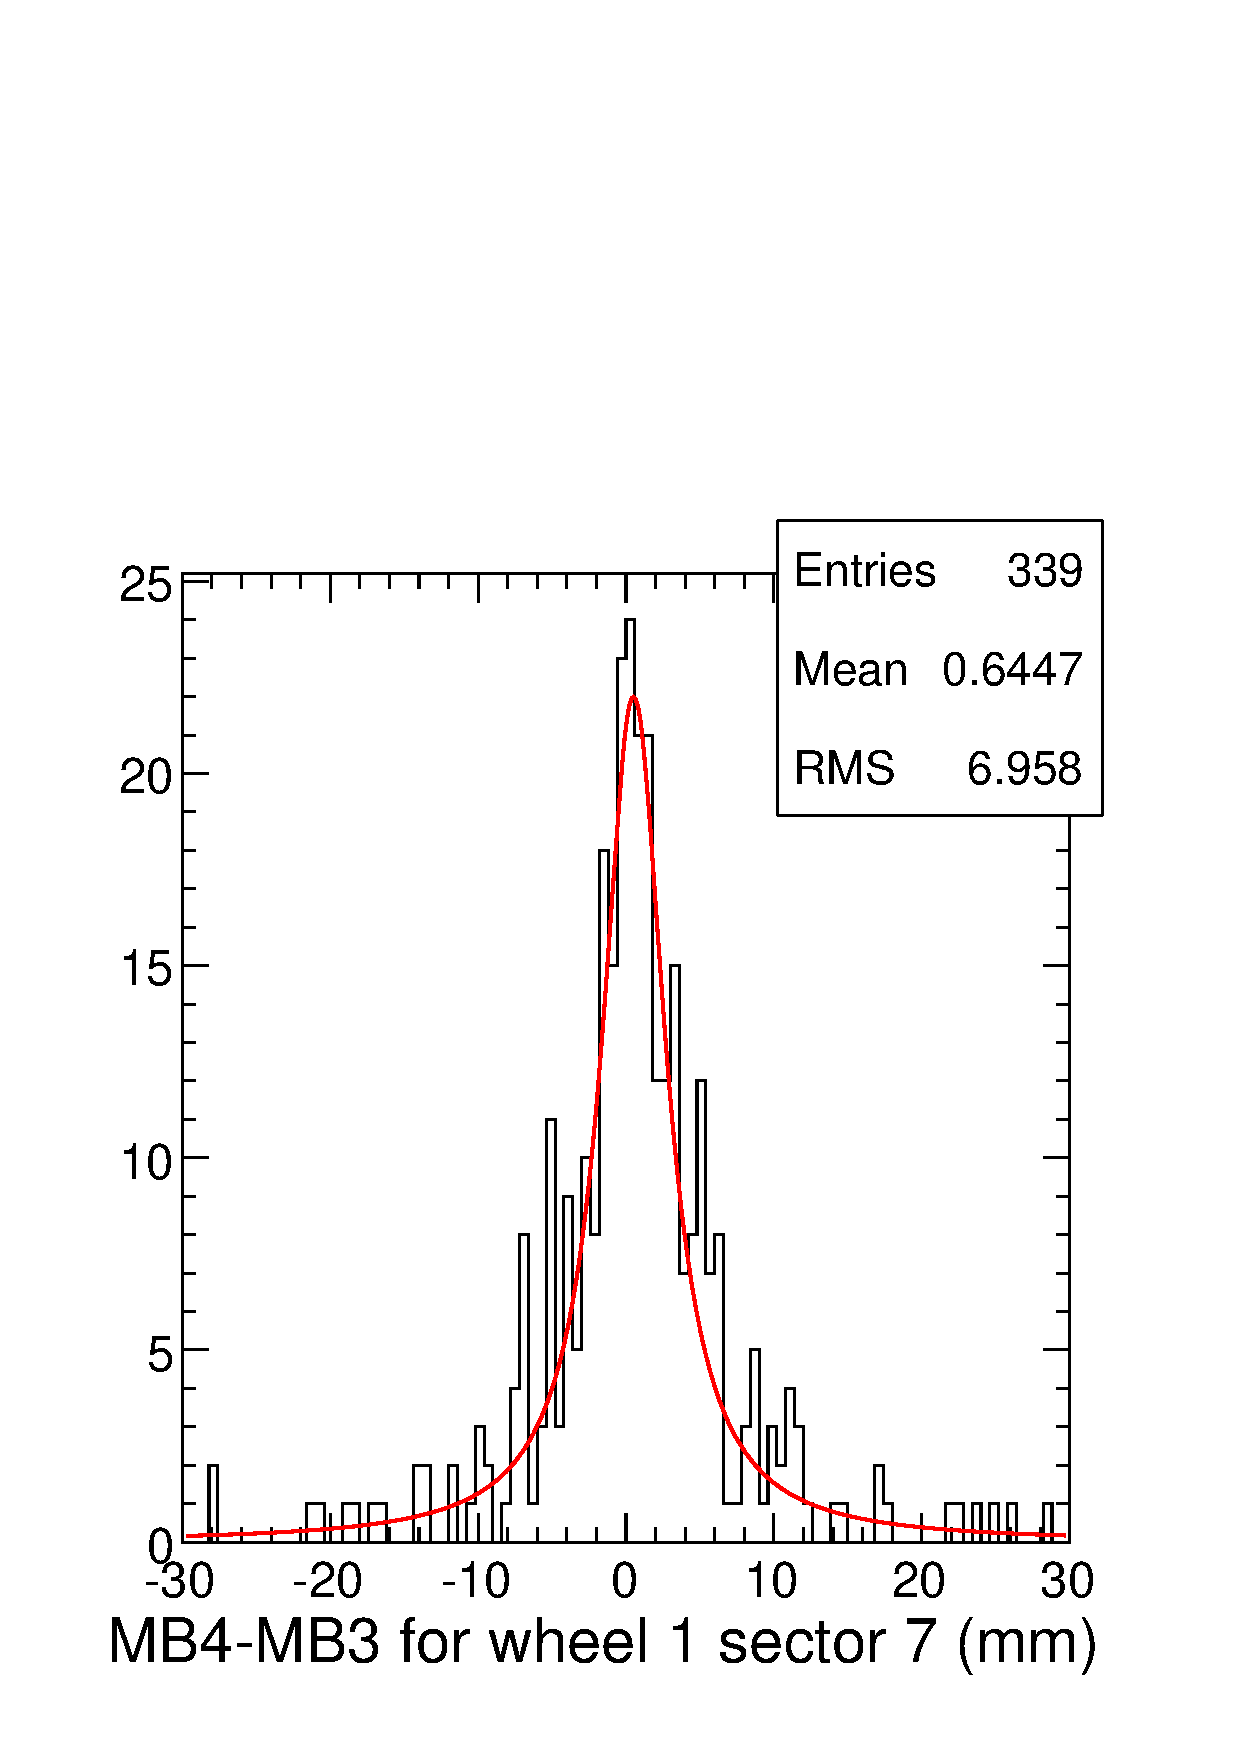
\includegraphics[width=0.25\linewidth]{diffindivphi_1_34_7.pdf}
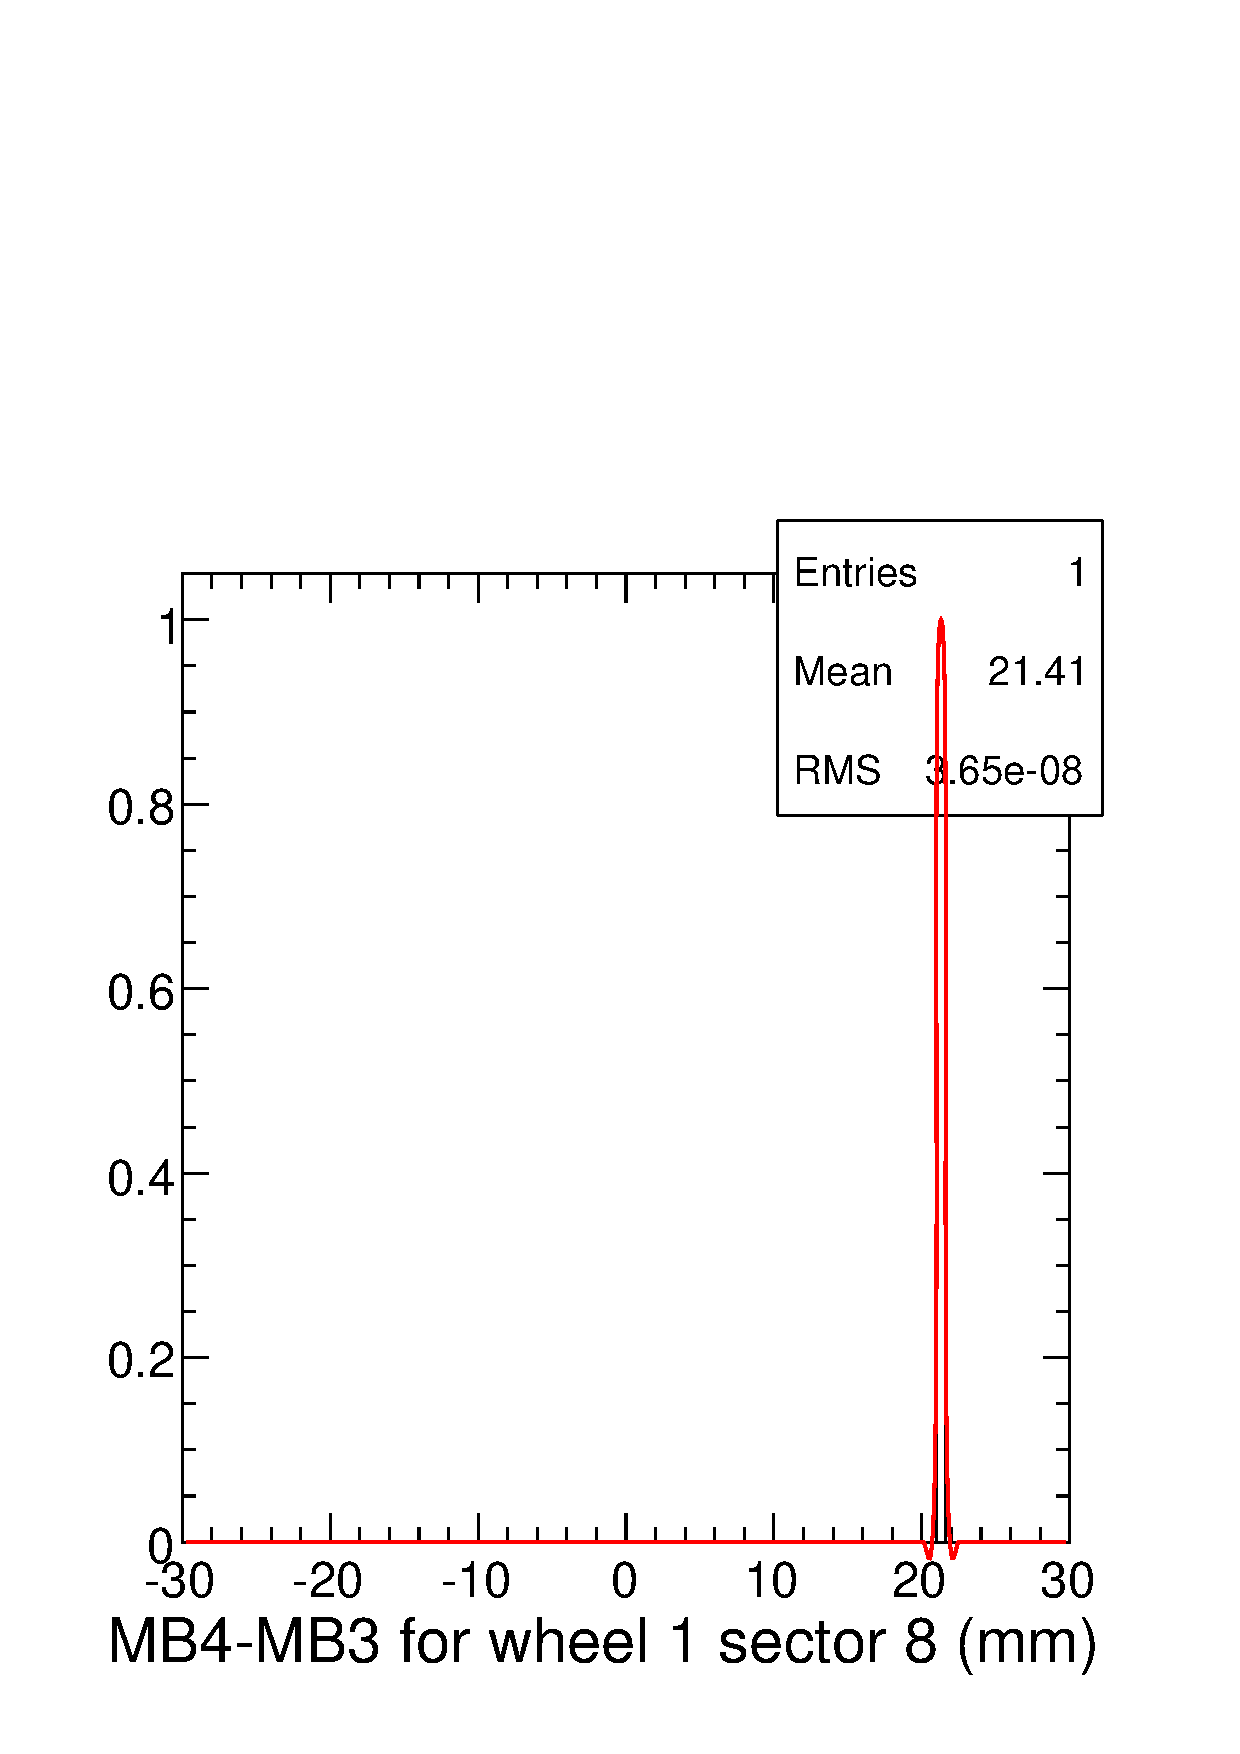
\includegraphics[width=0.25\linewidth]{diffindivphi_1_34_8.pdf}

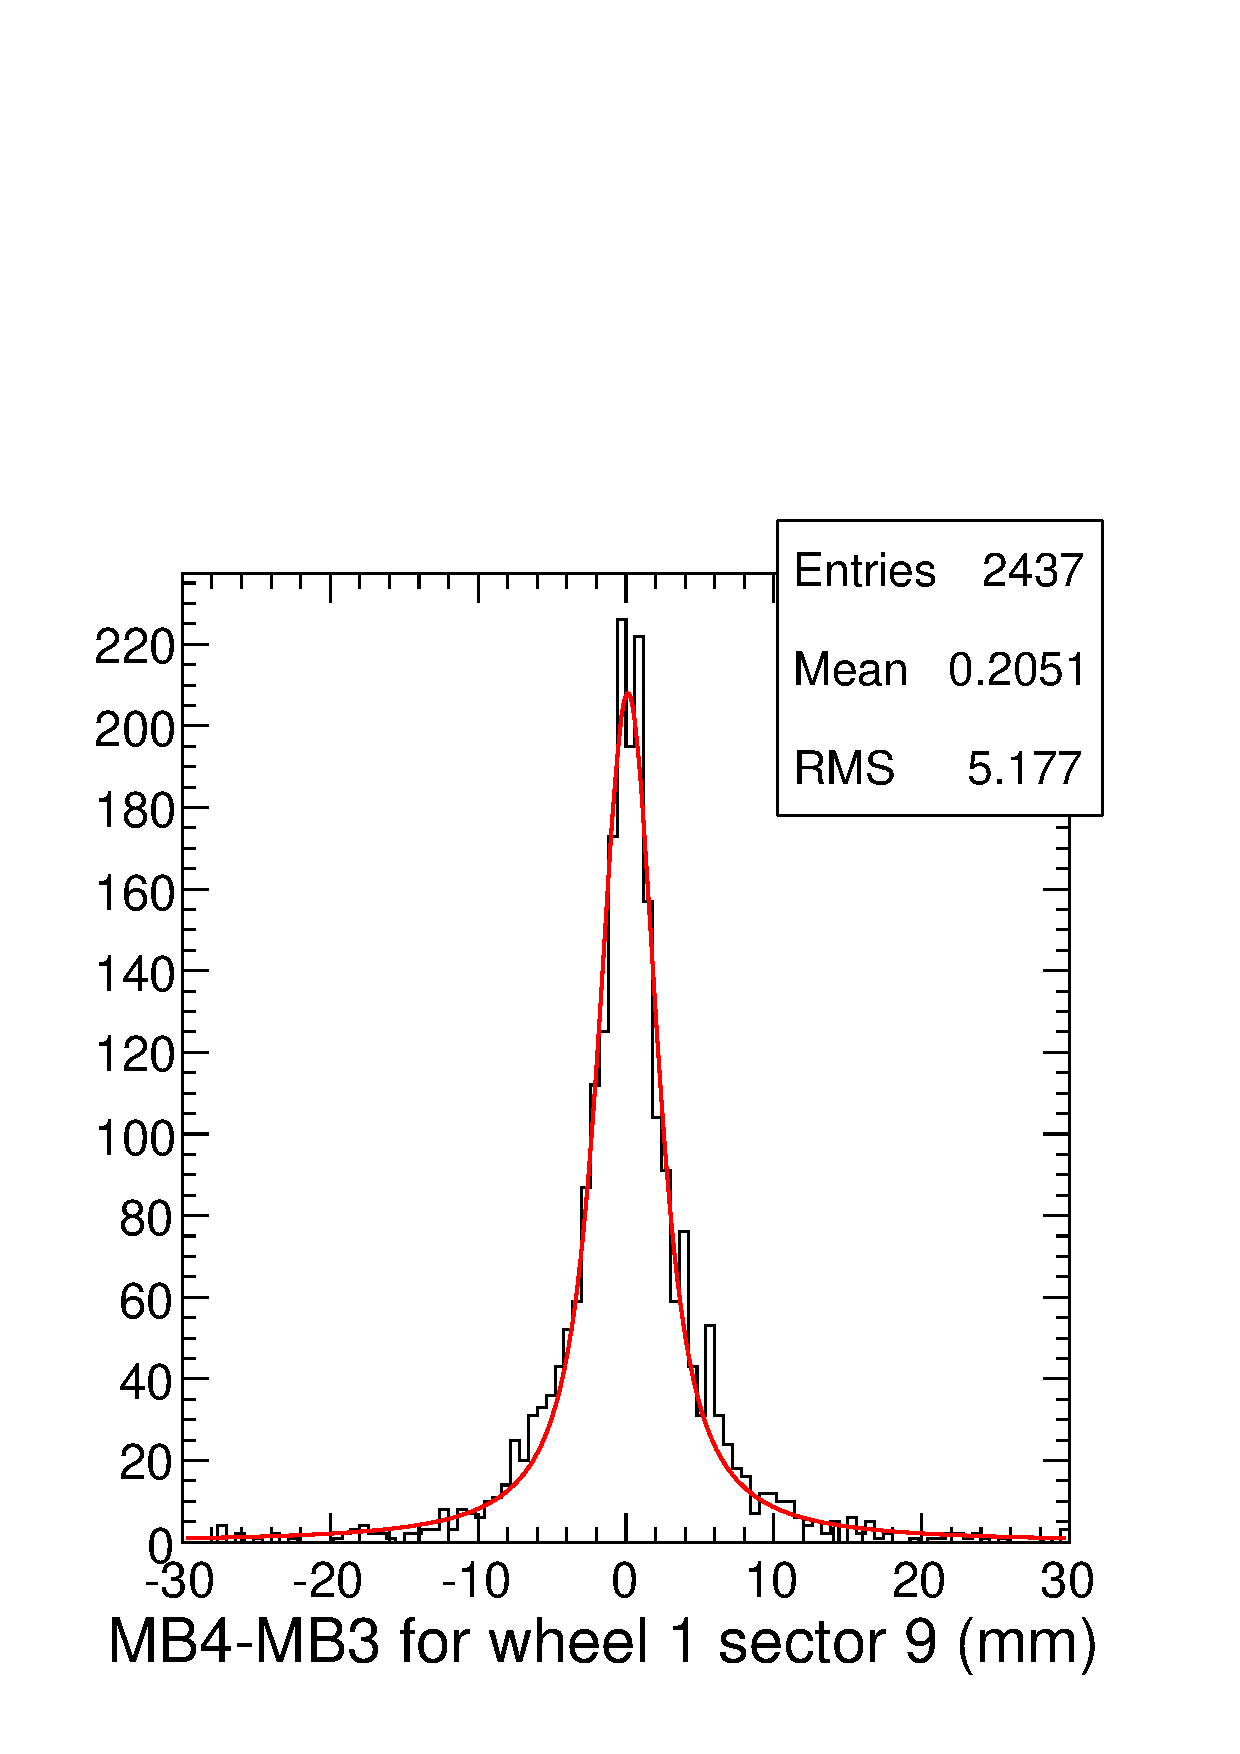
\includegraphics[width=0.25\linewidth]{diffindivphi_1_34_9.pdf}
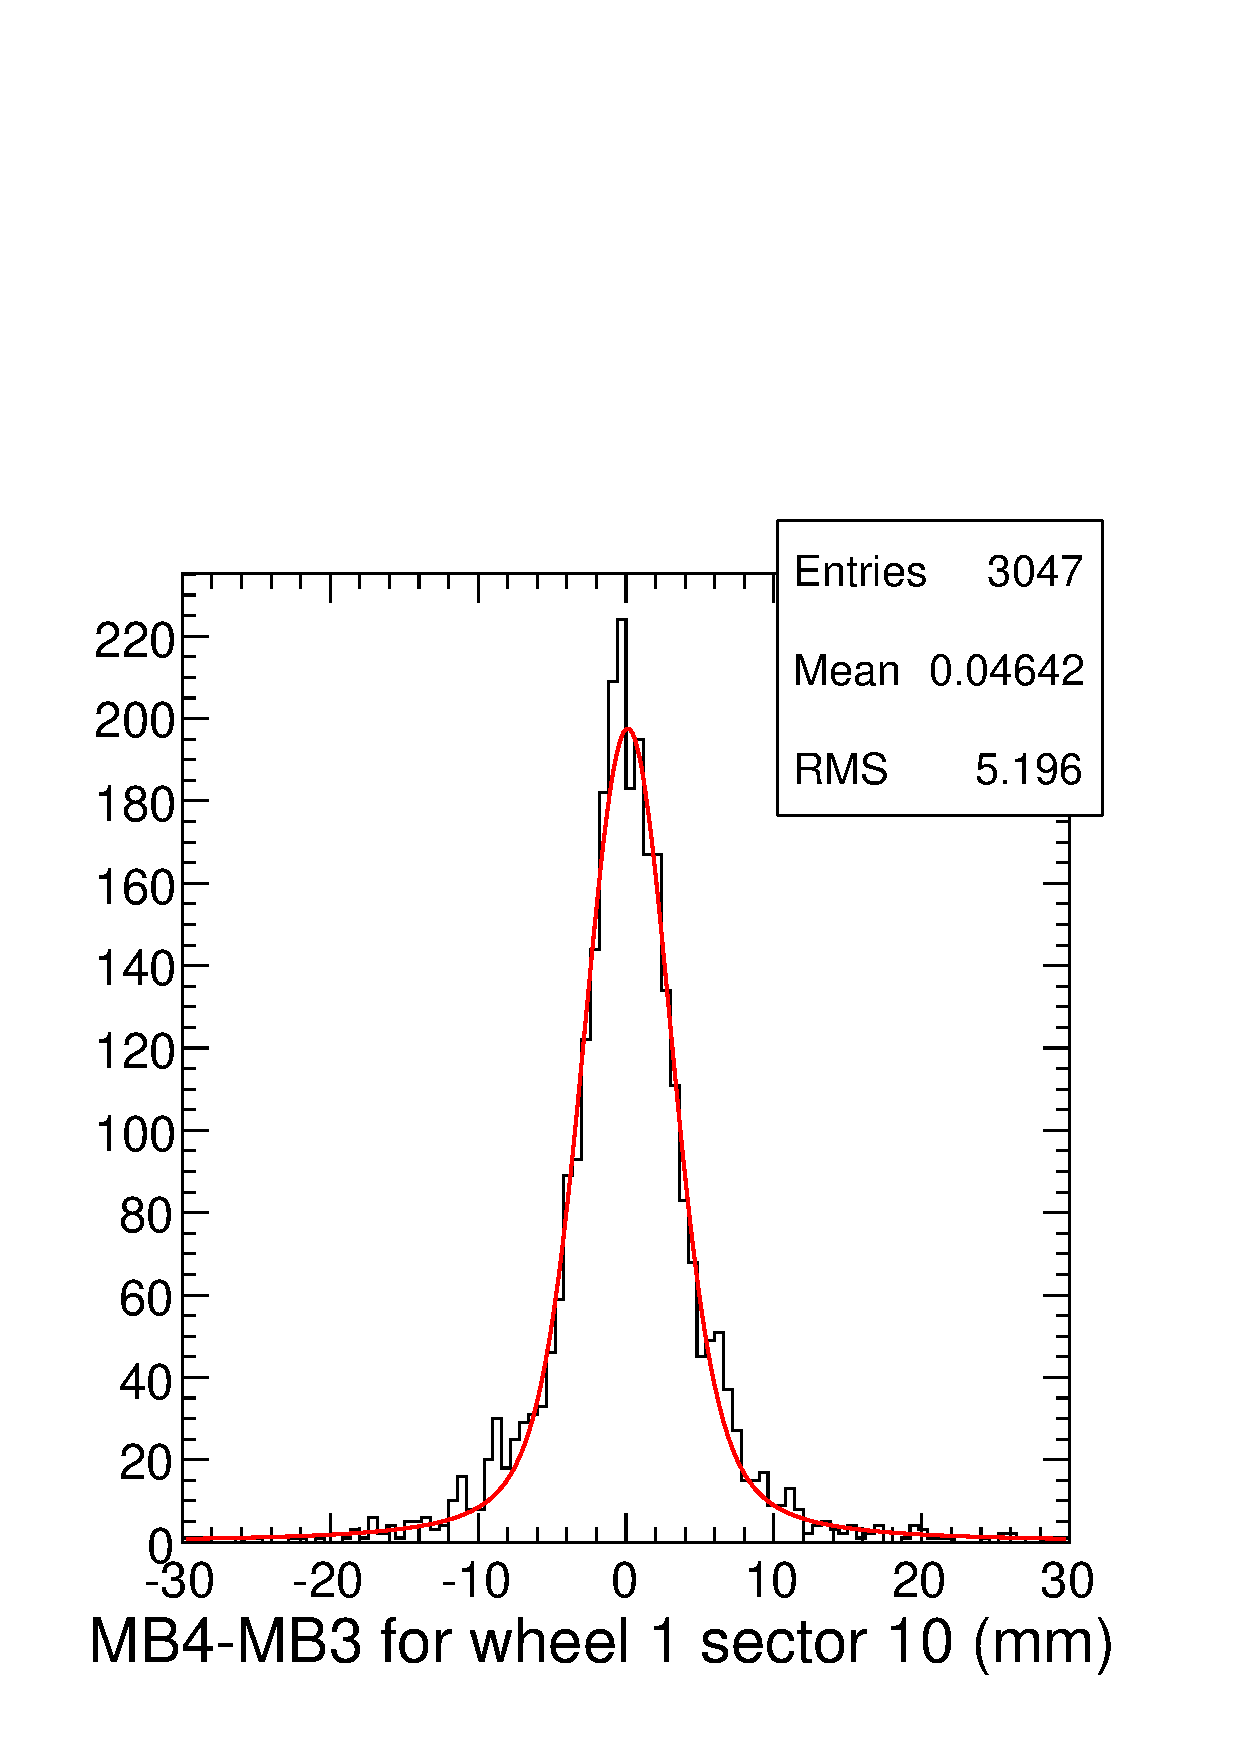
\includegraphics[width=0.25\linewidth]{diffindivphi_1_34_10.pdf}
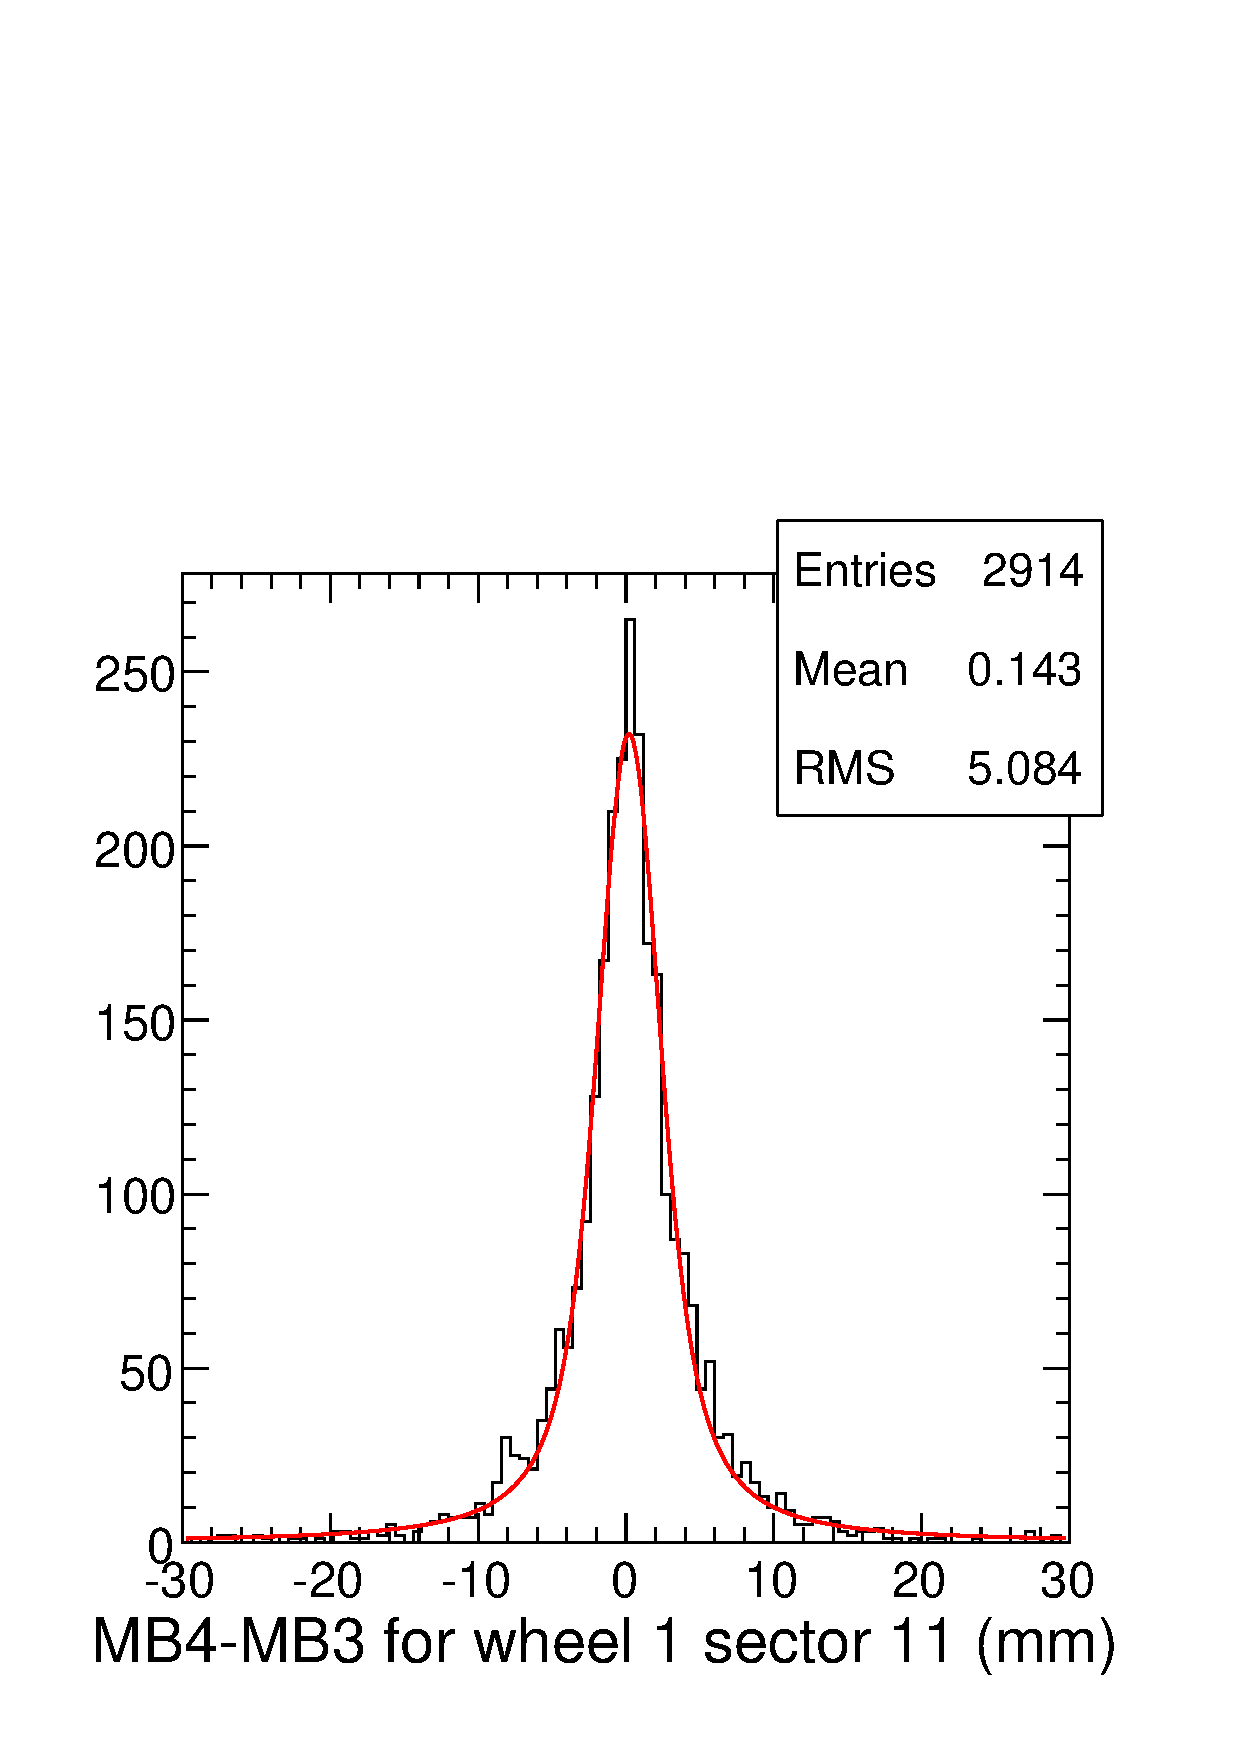
\includegraphics[width=0.25\linewidth]{diffindivphi_1_34_11.pdf}
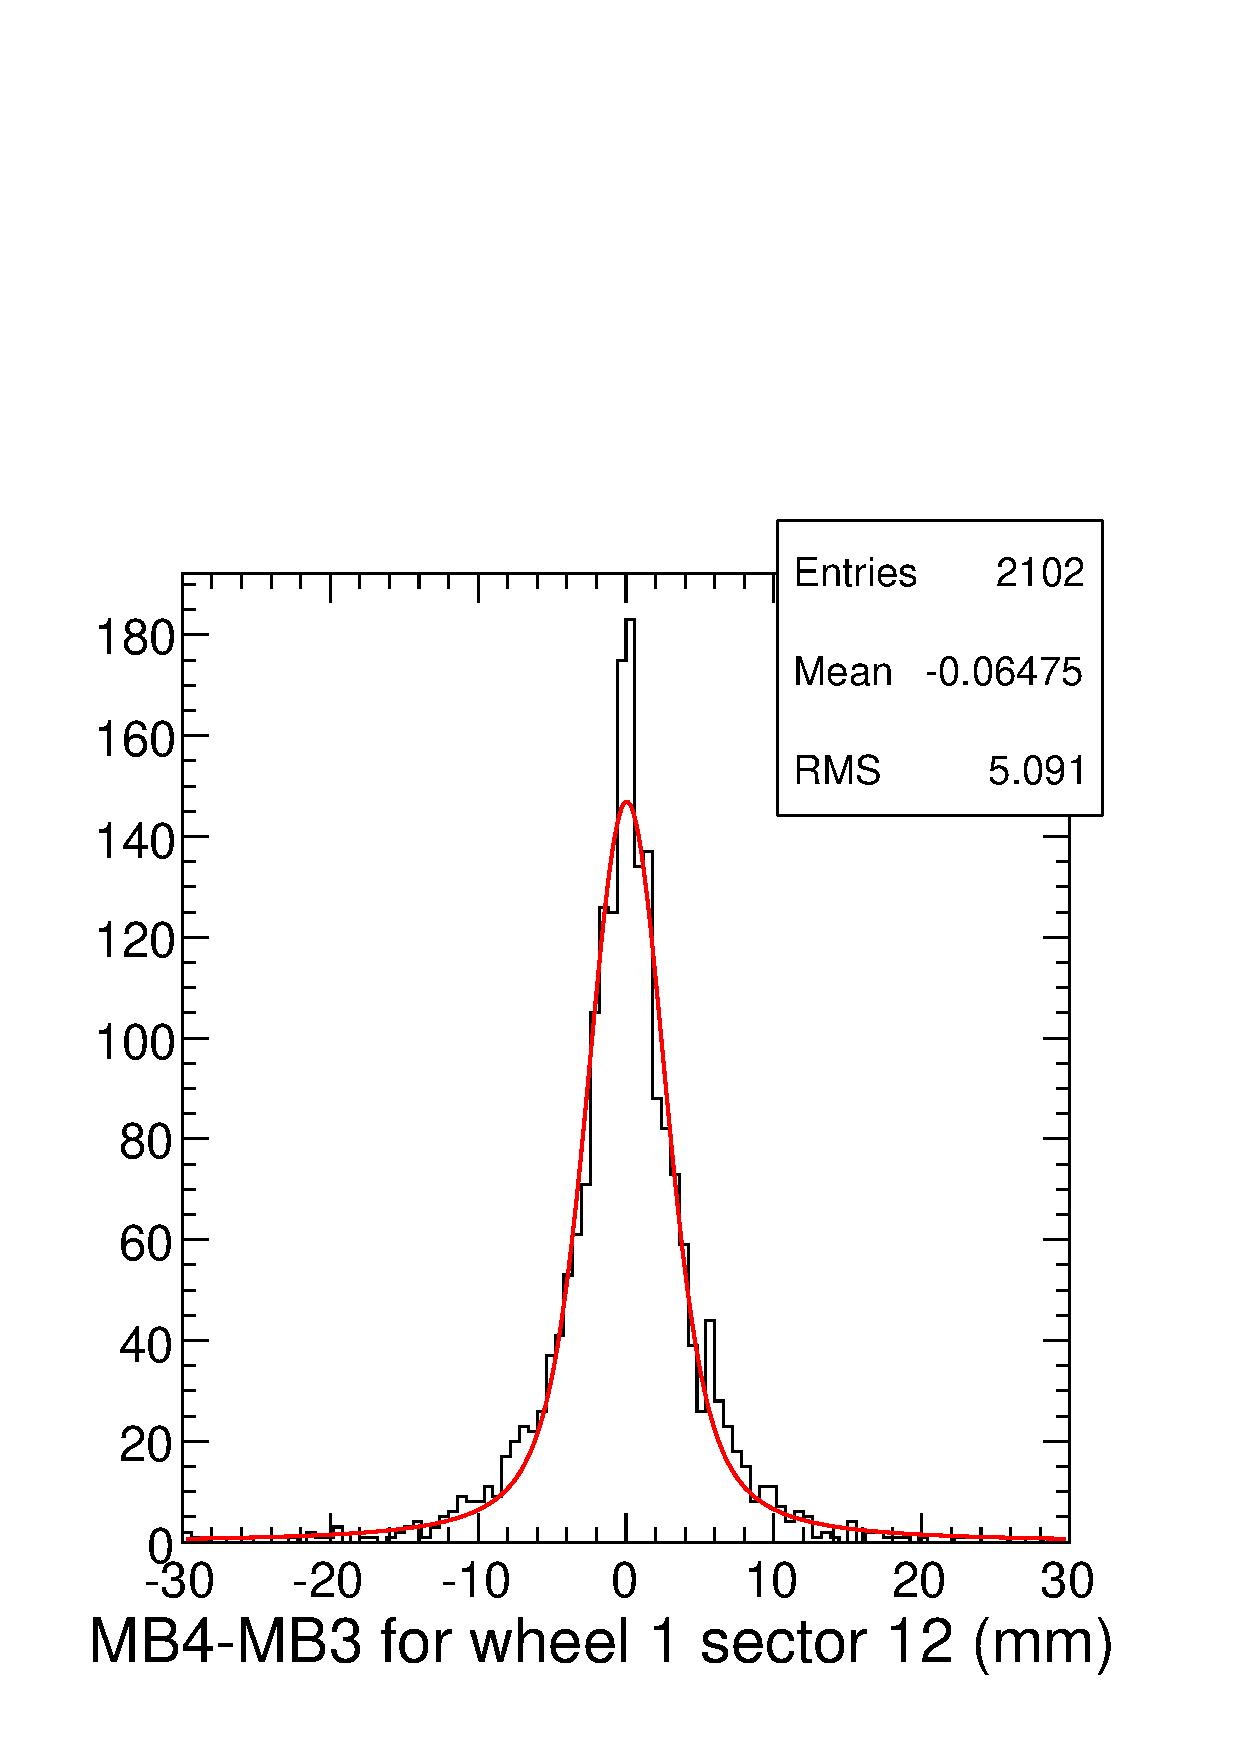
\includegraphics[width=0.25\linewidth]{diffindivphi_1_34_12.pdf}

\column{0.3\linewidth}
\scriptsize Chambers with too few tracks for alignment, such as sector 8, are excluded from the plots on the following pages
\end{columns}
\end{frame}

\begin{frame}
\frametitle{CRAFT\_ALL\_V4 $x$}

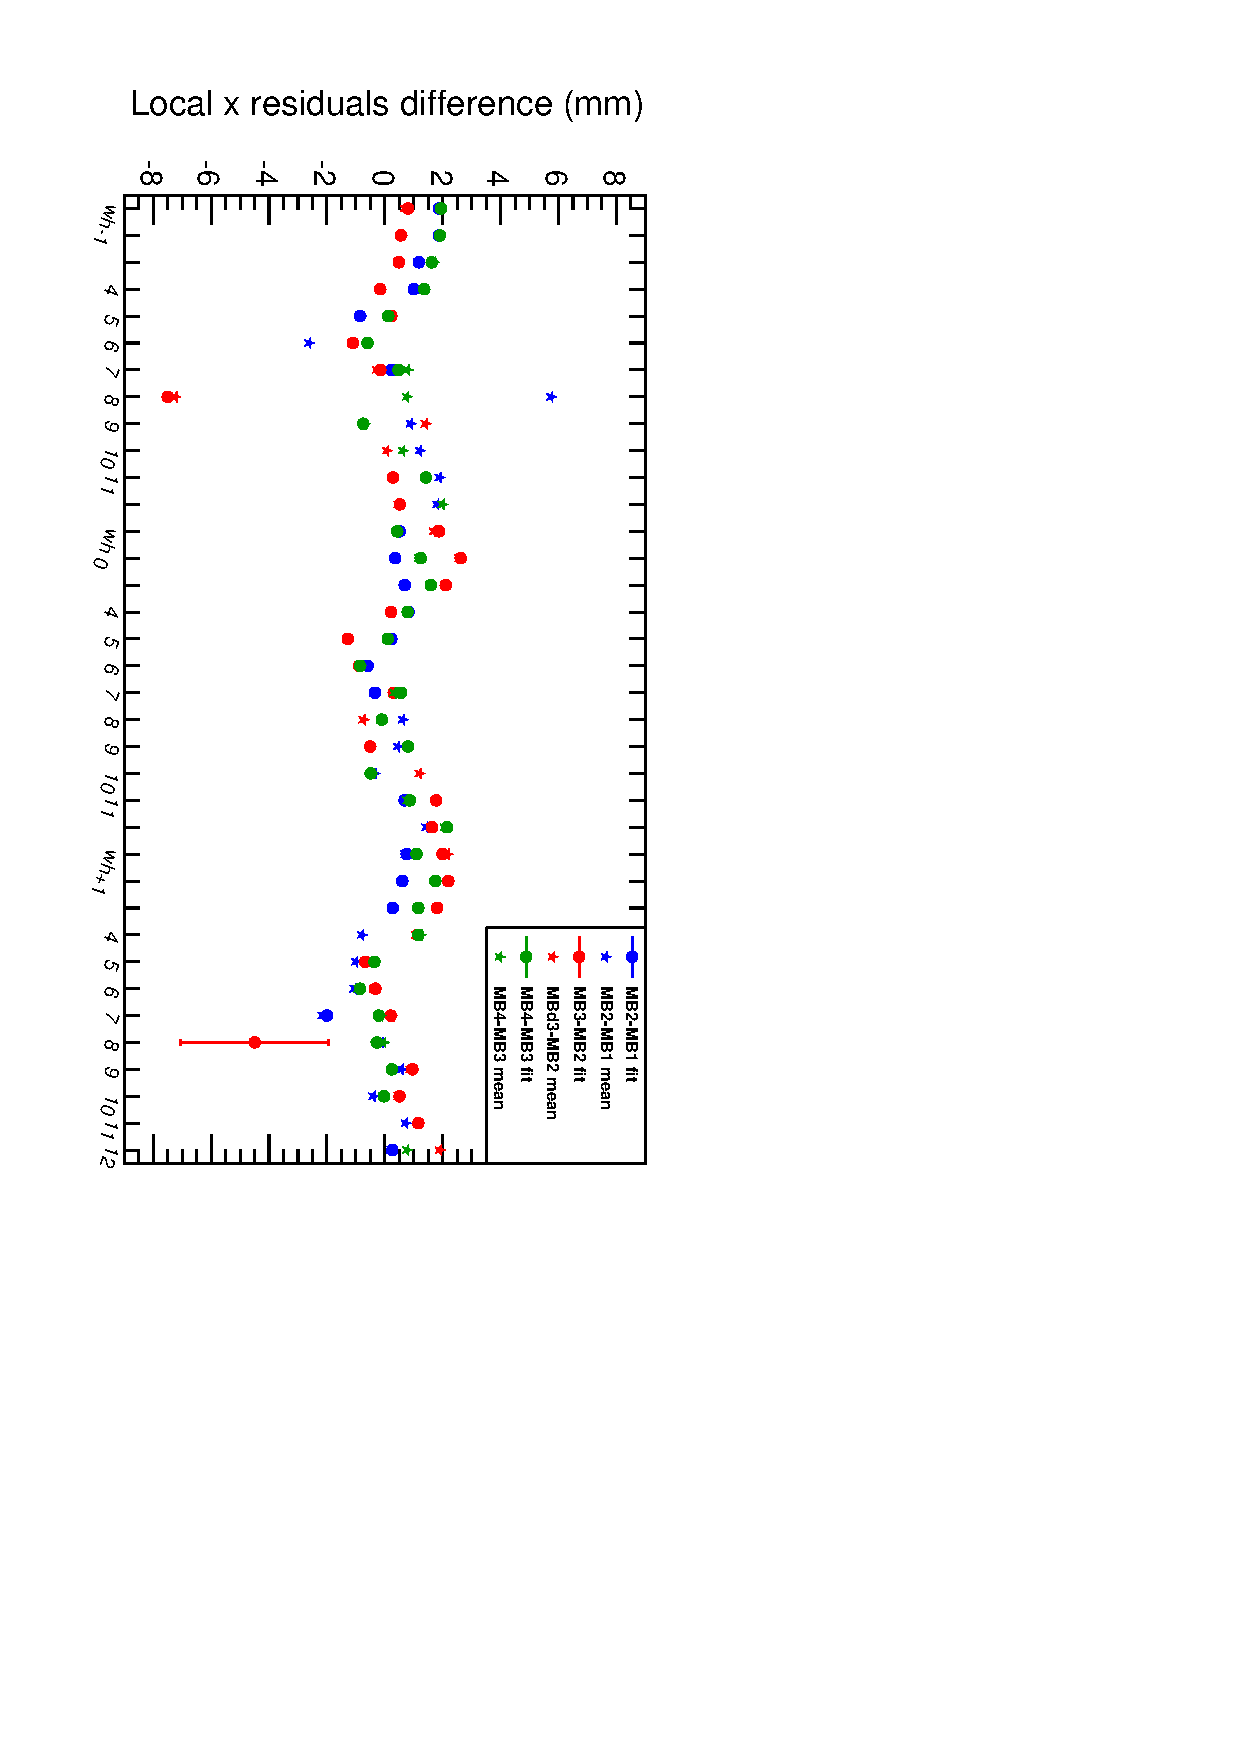
\includegraphics[width=4 cm, angle=90]{diffxsector_v4.pdf}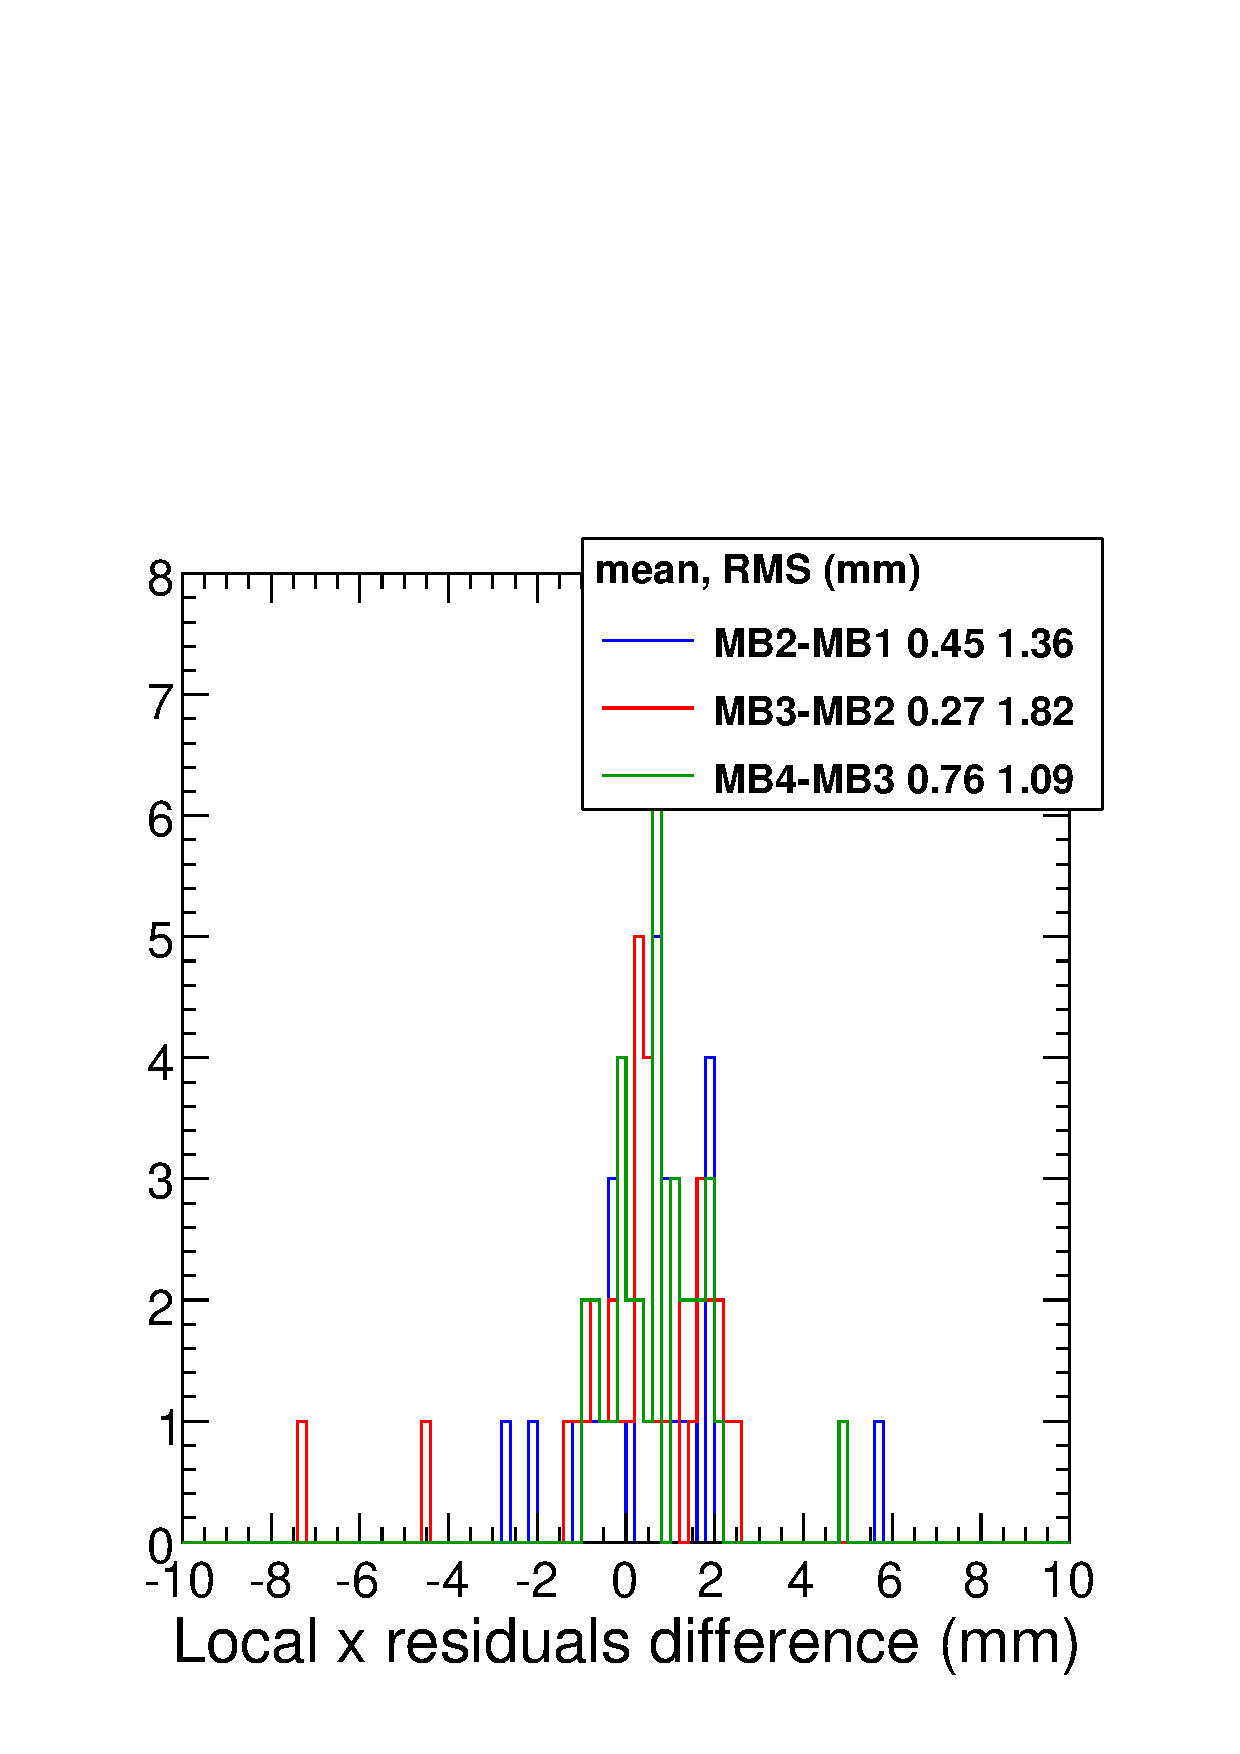
\includegraphics[height=4 cm]{diffxhist_v4.pdf}

\vfill
\hspace{-0.83 cm} \textcolor{darkblue}{\Large CRAFT\_ALL\_V4 $\phi_y$}

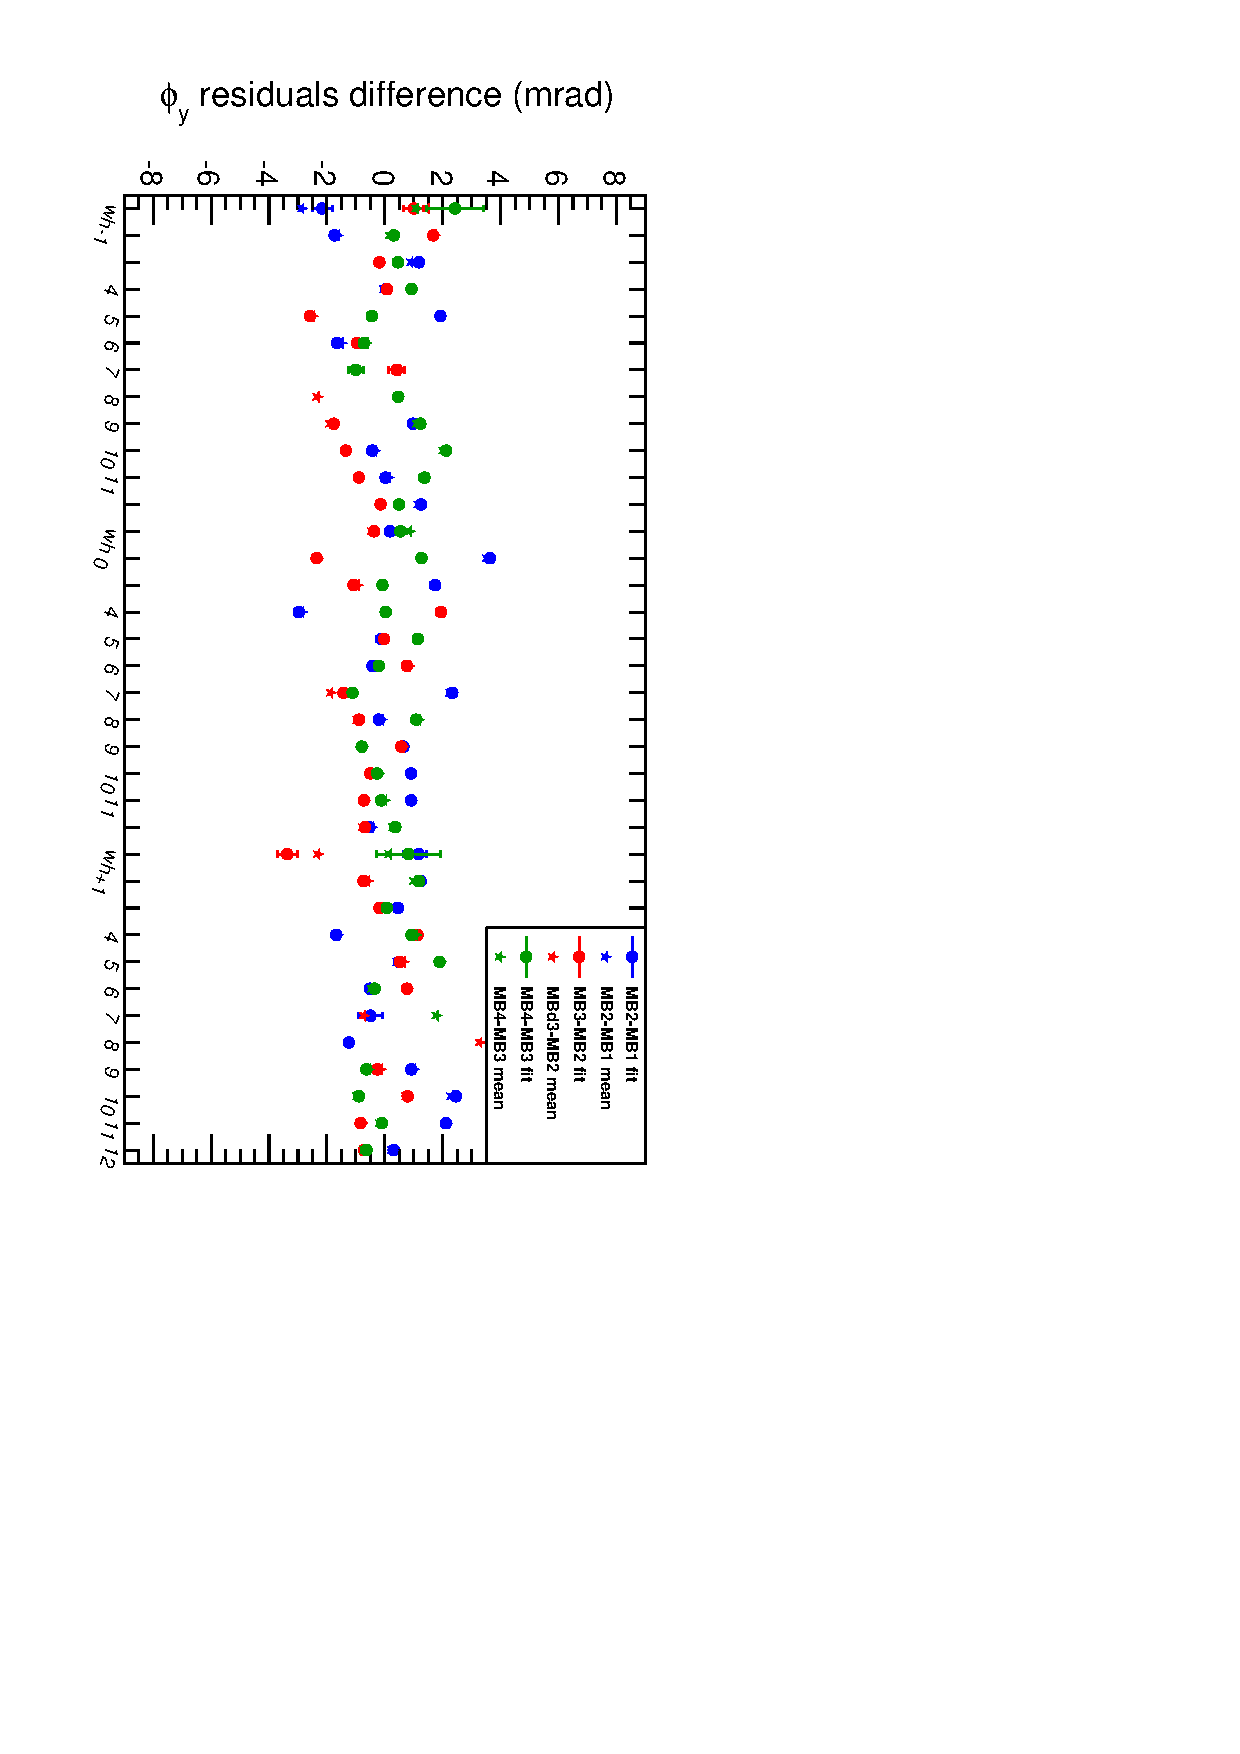
\includegraphics[width=4 cm, angle=90]{diffphisector_v4.pdf}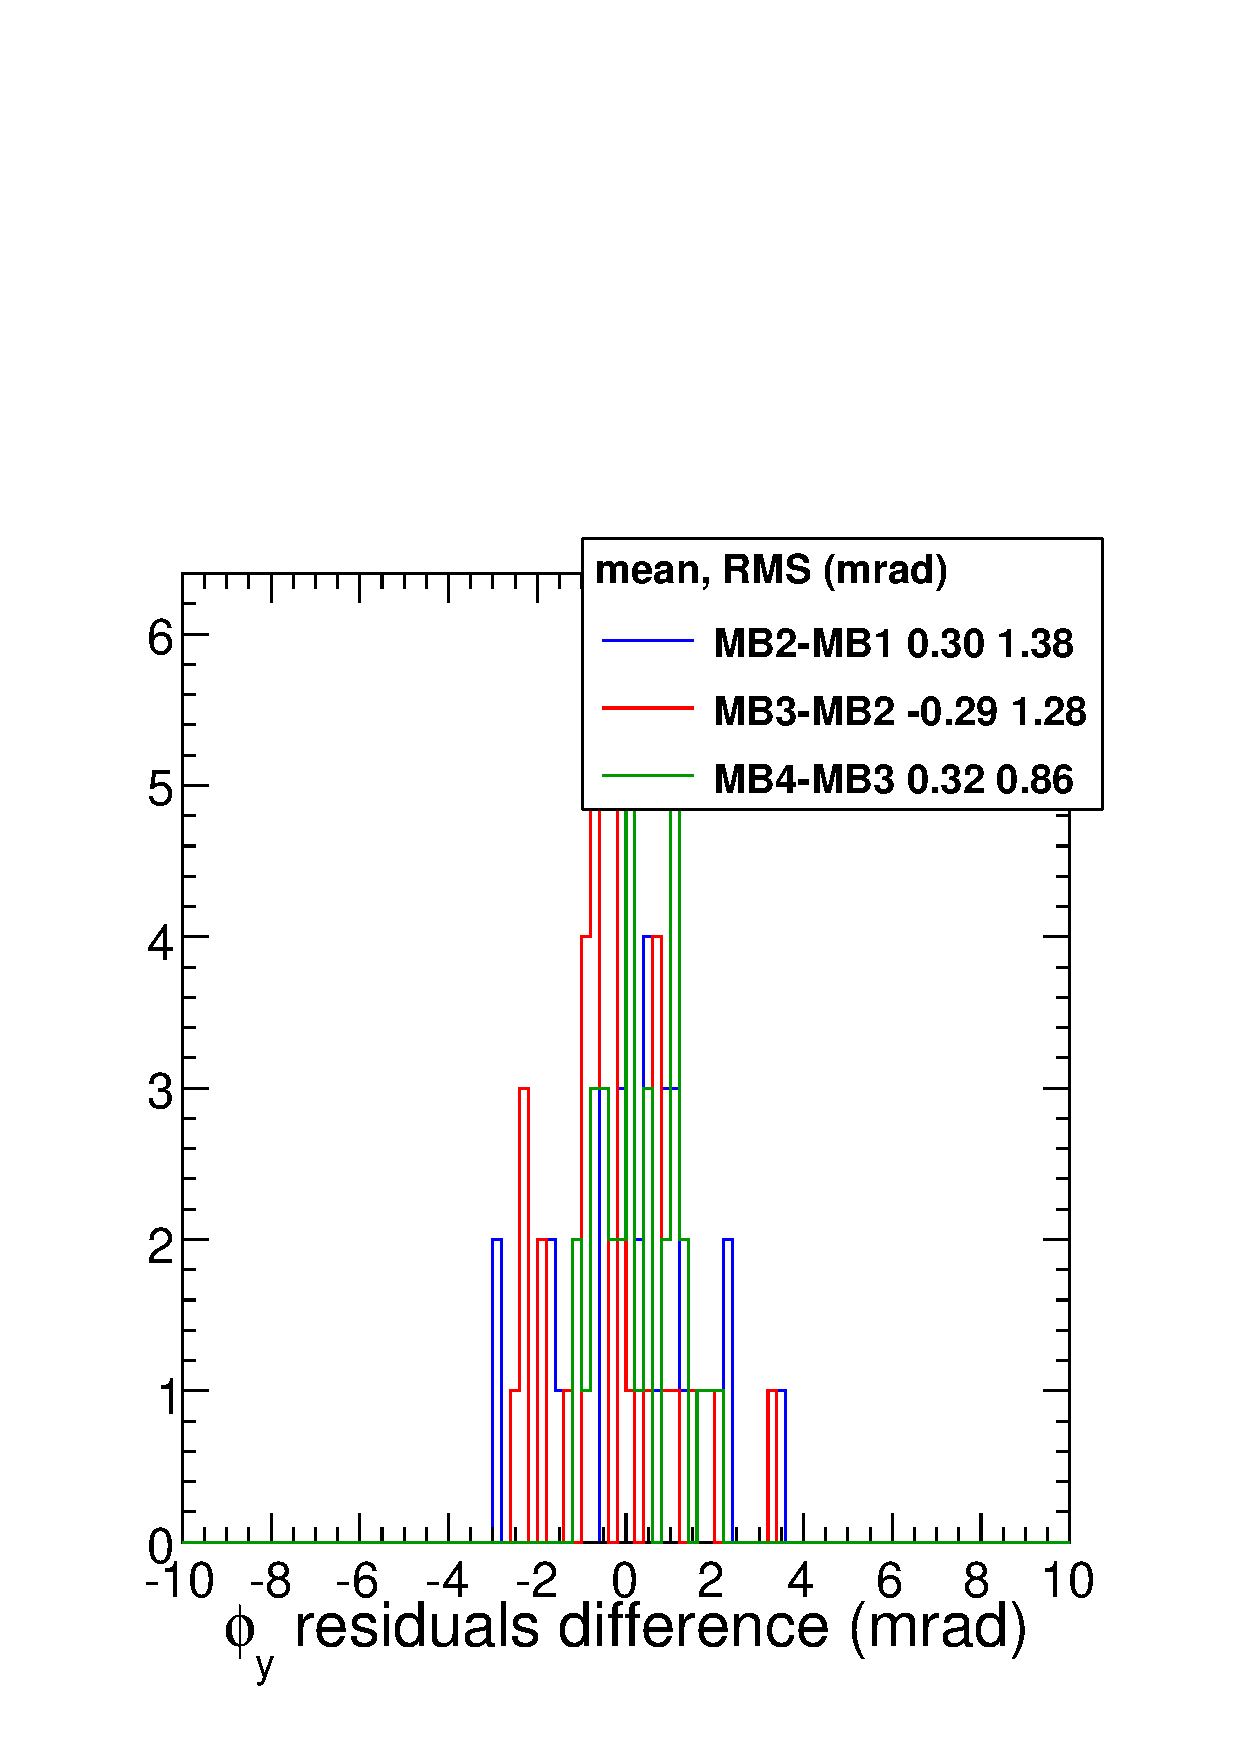
\includegraphics[height=4 cm]{diffphihist_v4.pdf}
\end{frame}

\begin{frame}
\frametitle{CRAFT\_ALL\_V11 $x$}

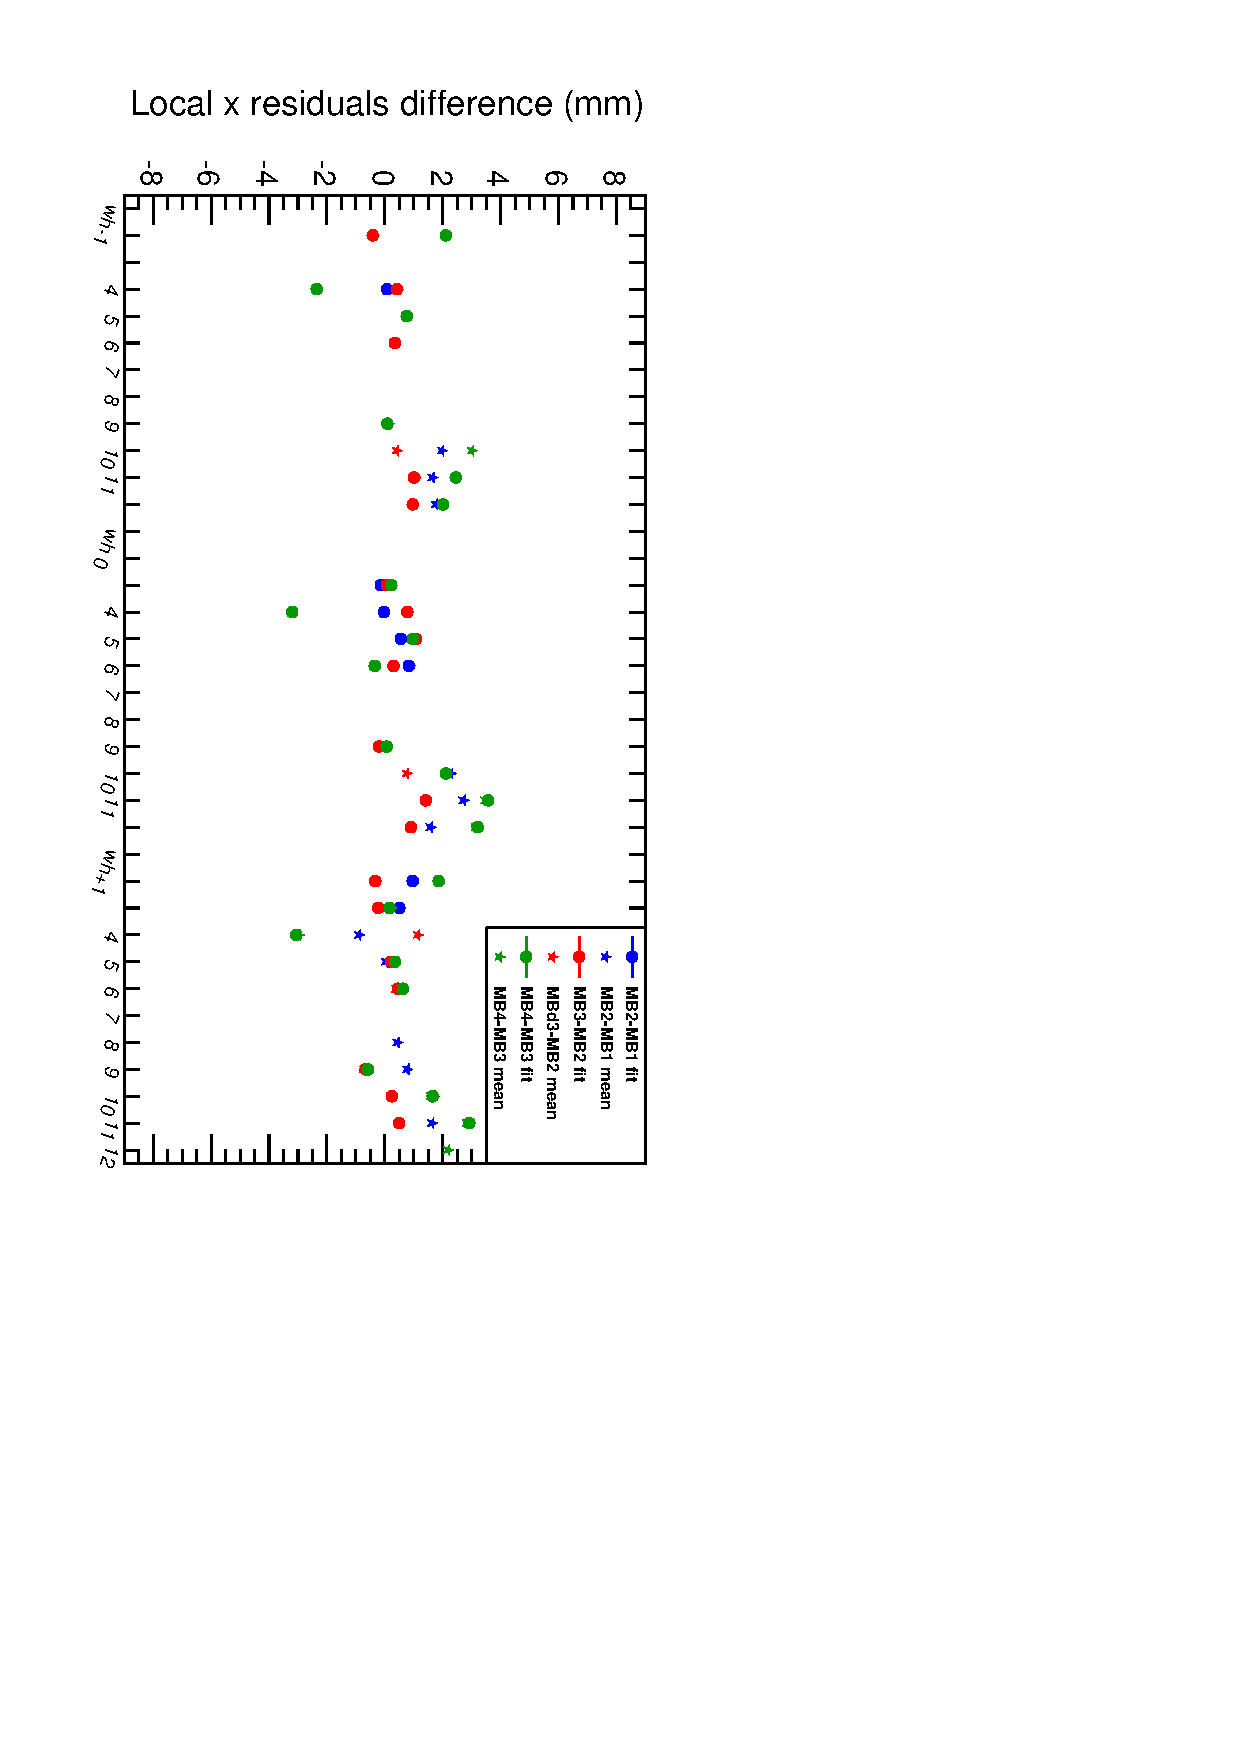
\includegraphics[width=4 cm, angle=90]{diffxsector_v11.pdf}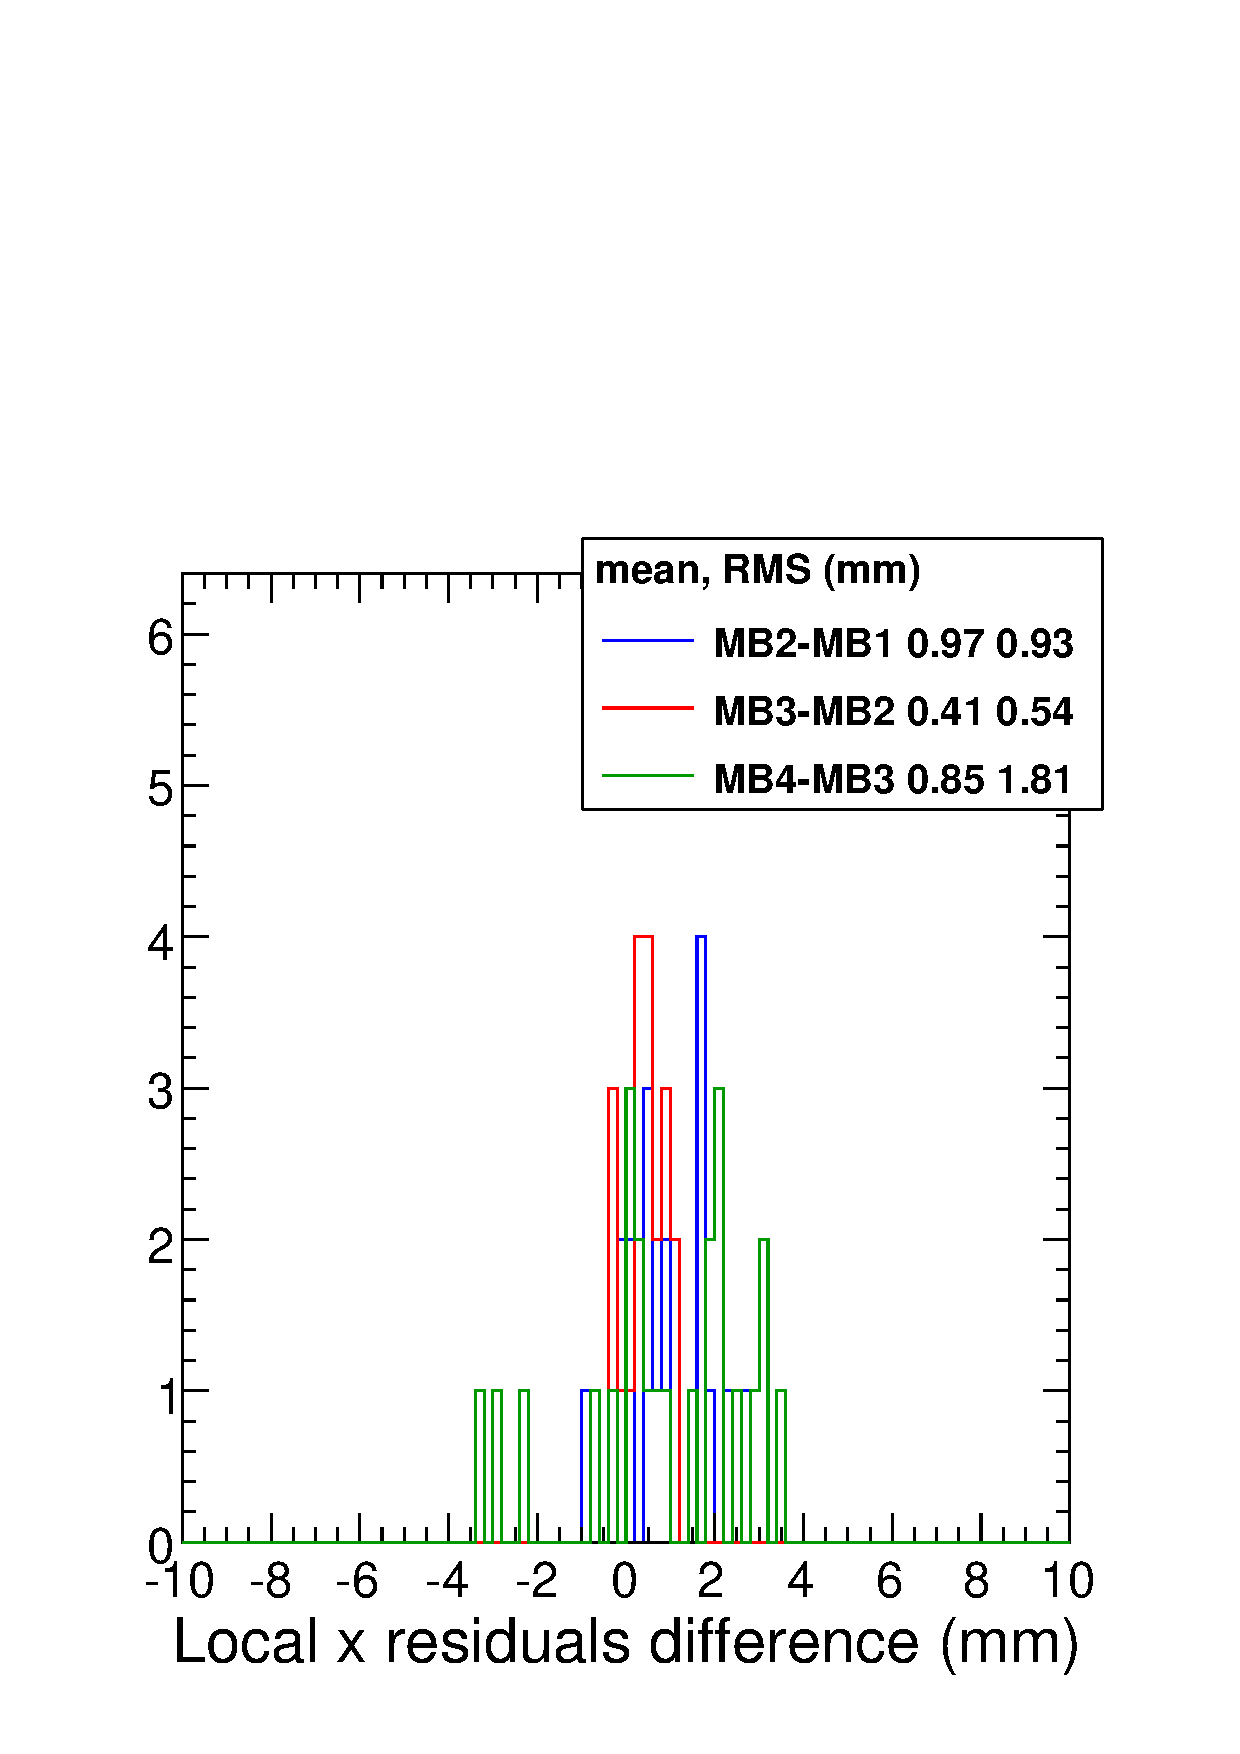
\includegraphics[height=4 cm]{diffxhist_v11.pdf}

\vfill
\hspace{-0.83 cm} \textcolor{darkblue}{\Large CRAFT\_ALL\_V11 $\phi_y$}

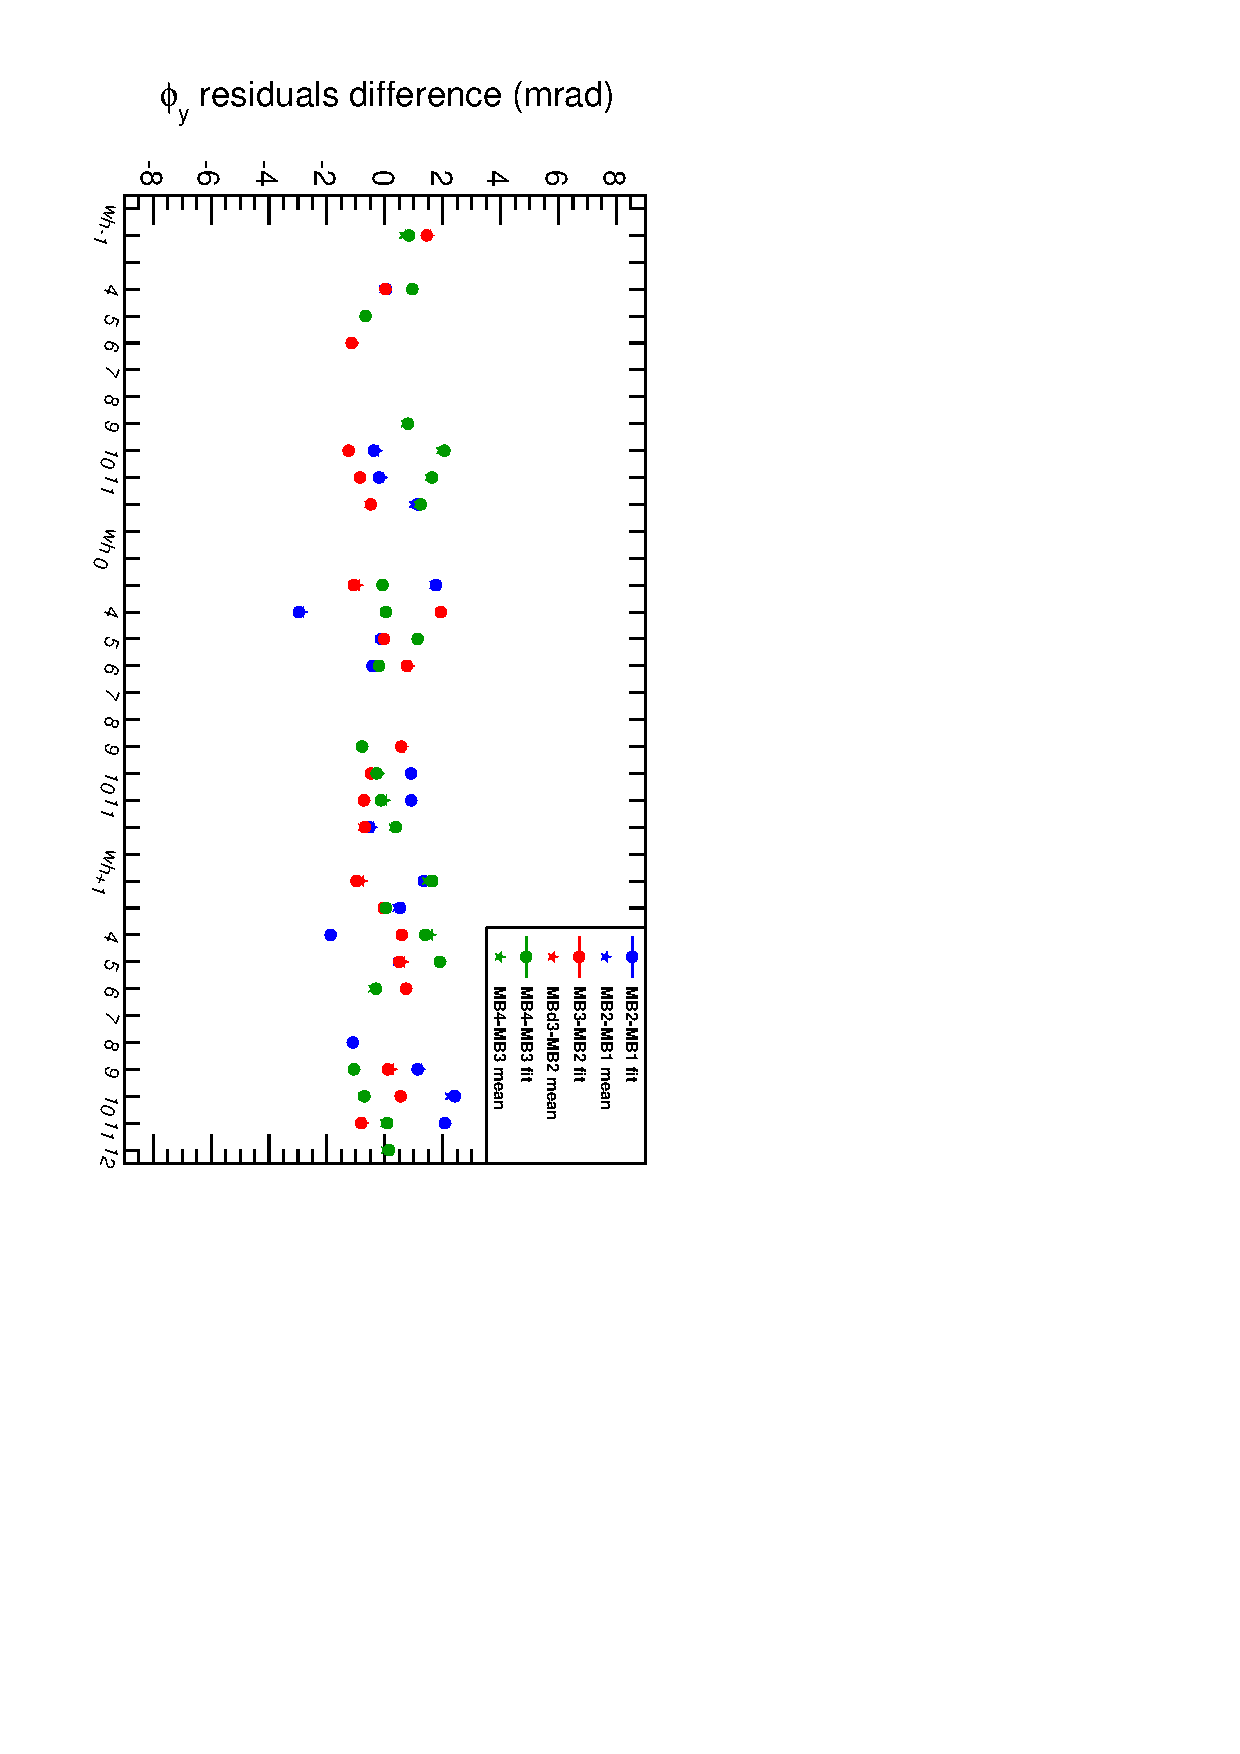
\includegraphics[width=4 cm, angle=90]{diffphisector_v11.pdf}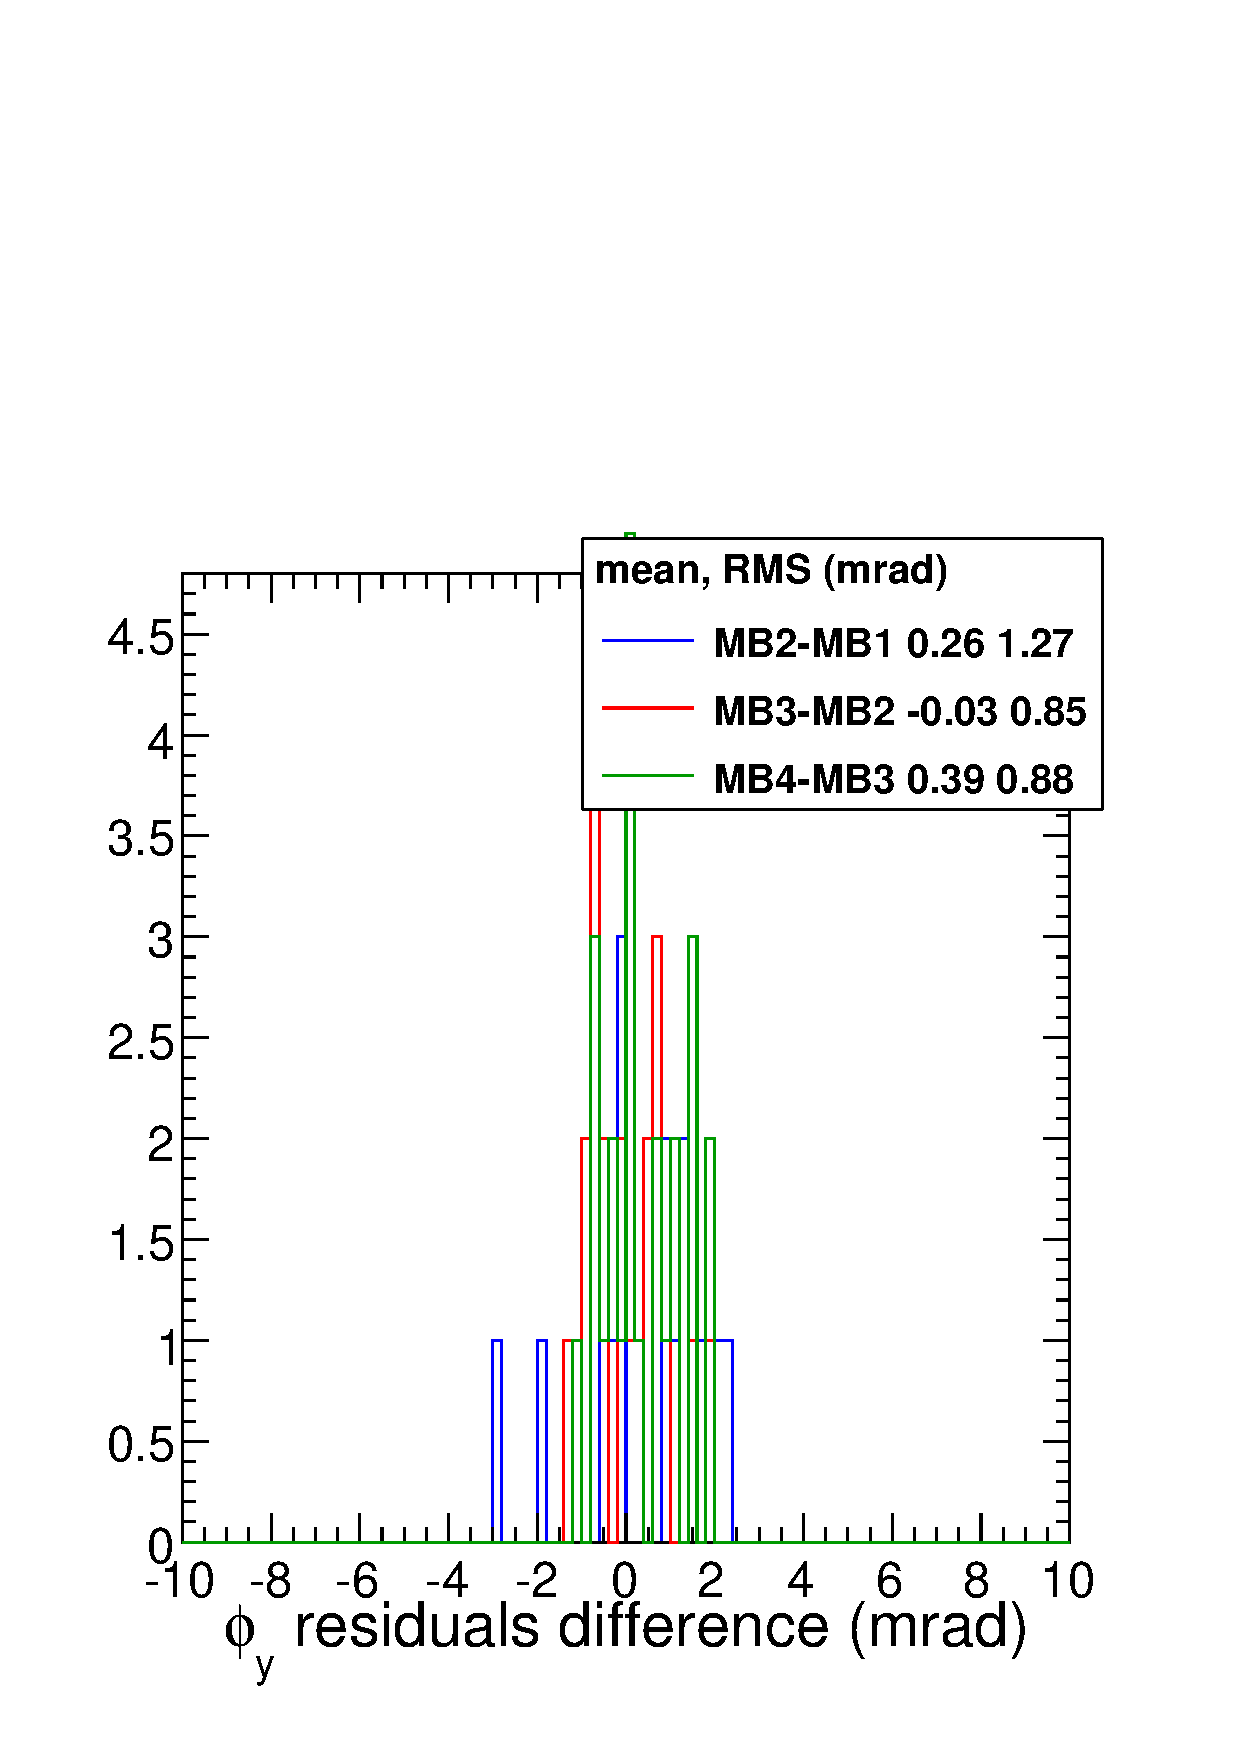
\includegraphics[height=4 cm]{diffphihist_v11.pdf}
\end{frame}

\begin{frame}
\frametitle{May 25 $x$}

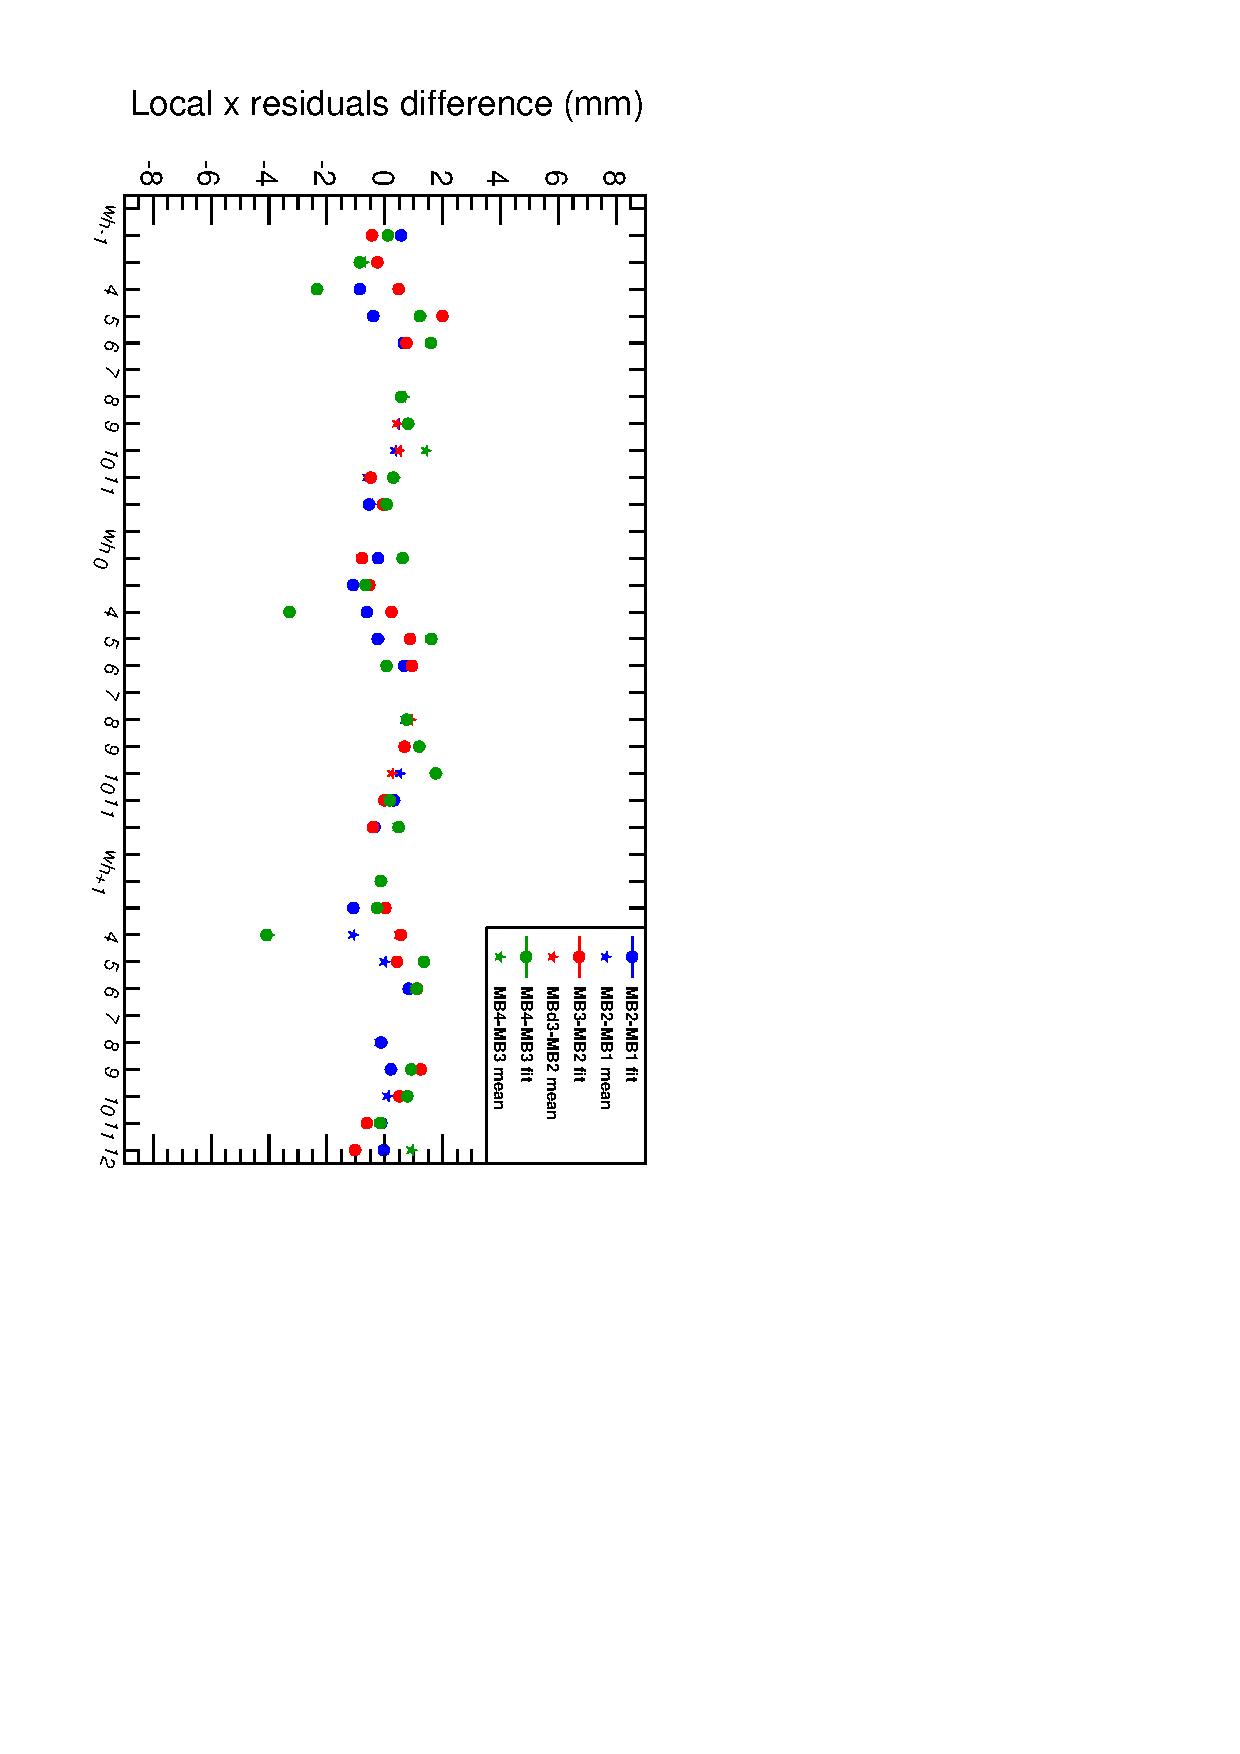
\includegraphics[width=4 cm, angle=90]{diffxsector_may25.pdf}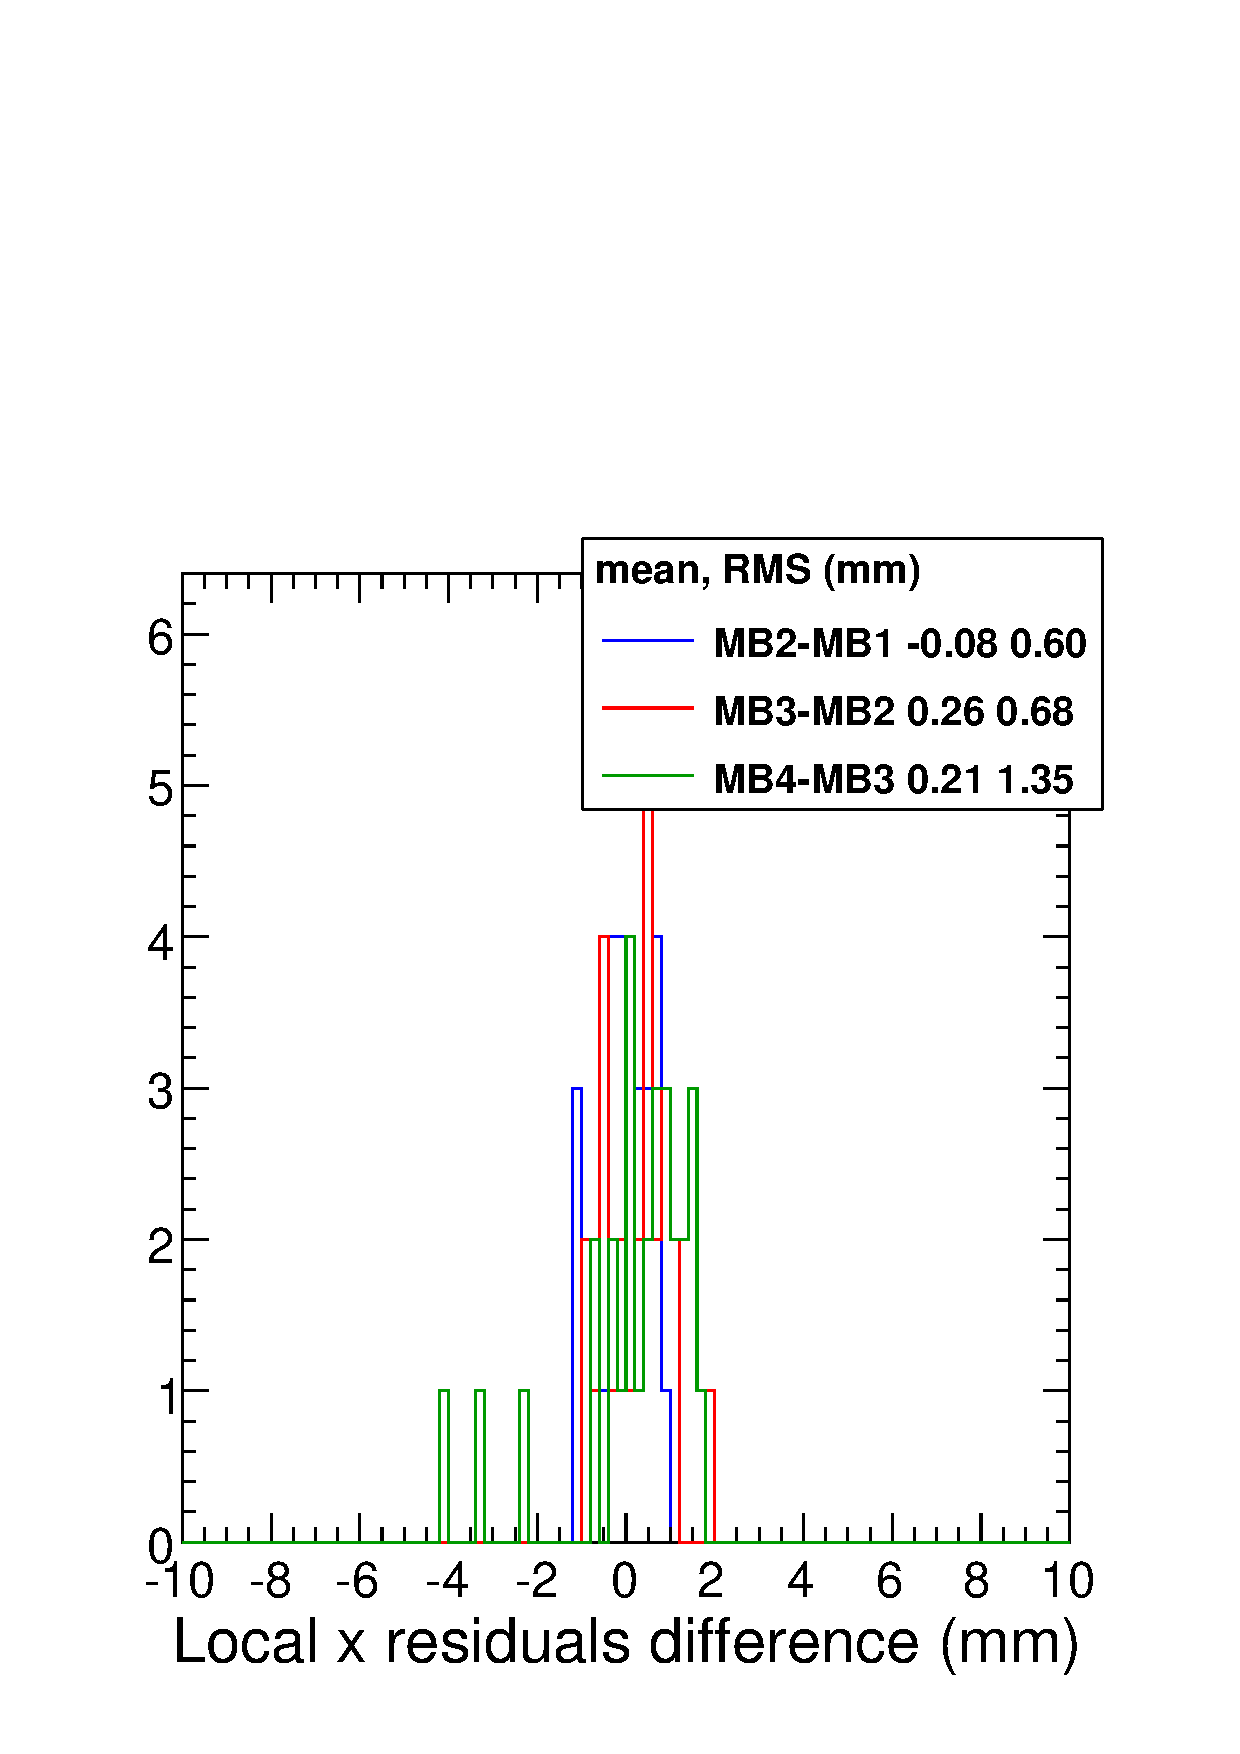
\includegraphics[height=4 cm]{diffxhist_may25.pdf}

\vfill
\hspace{-0.83 cm} \textcolor{darkblue}{\Large May 25 $\phi_y$}

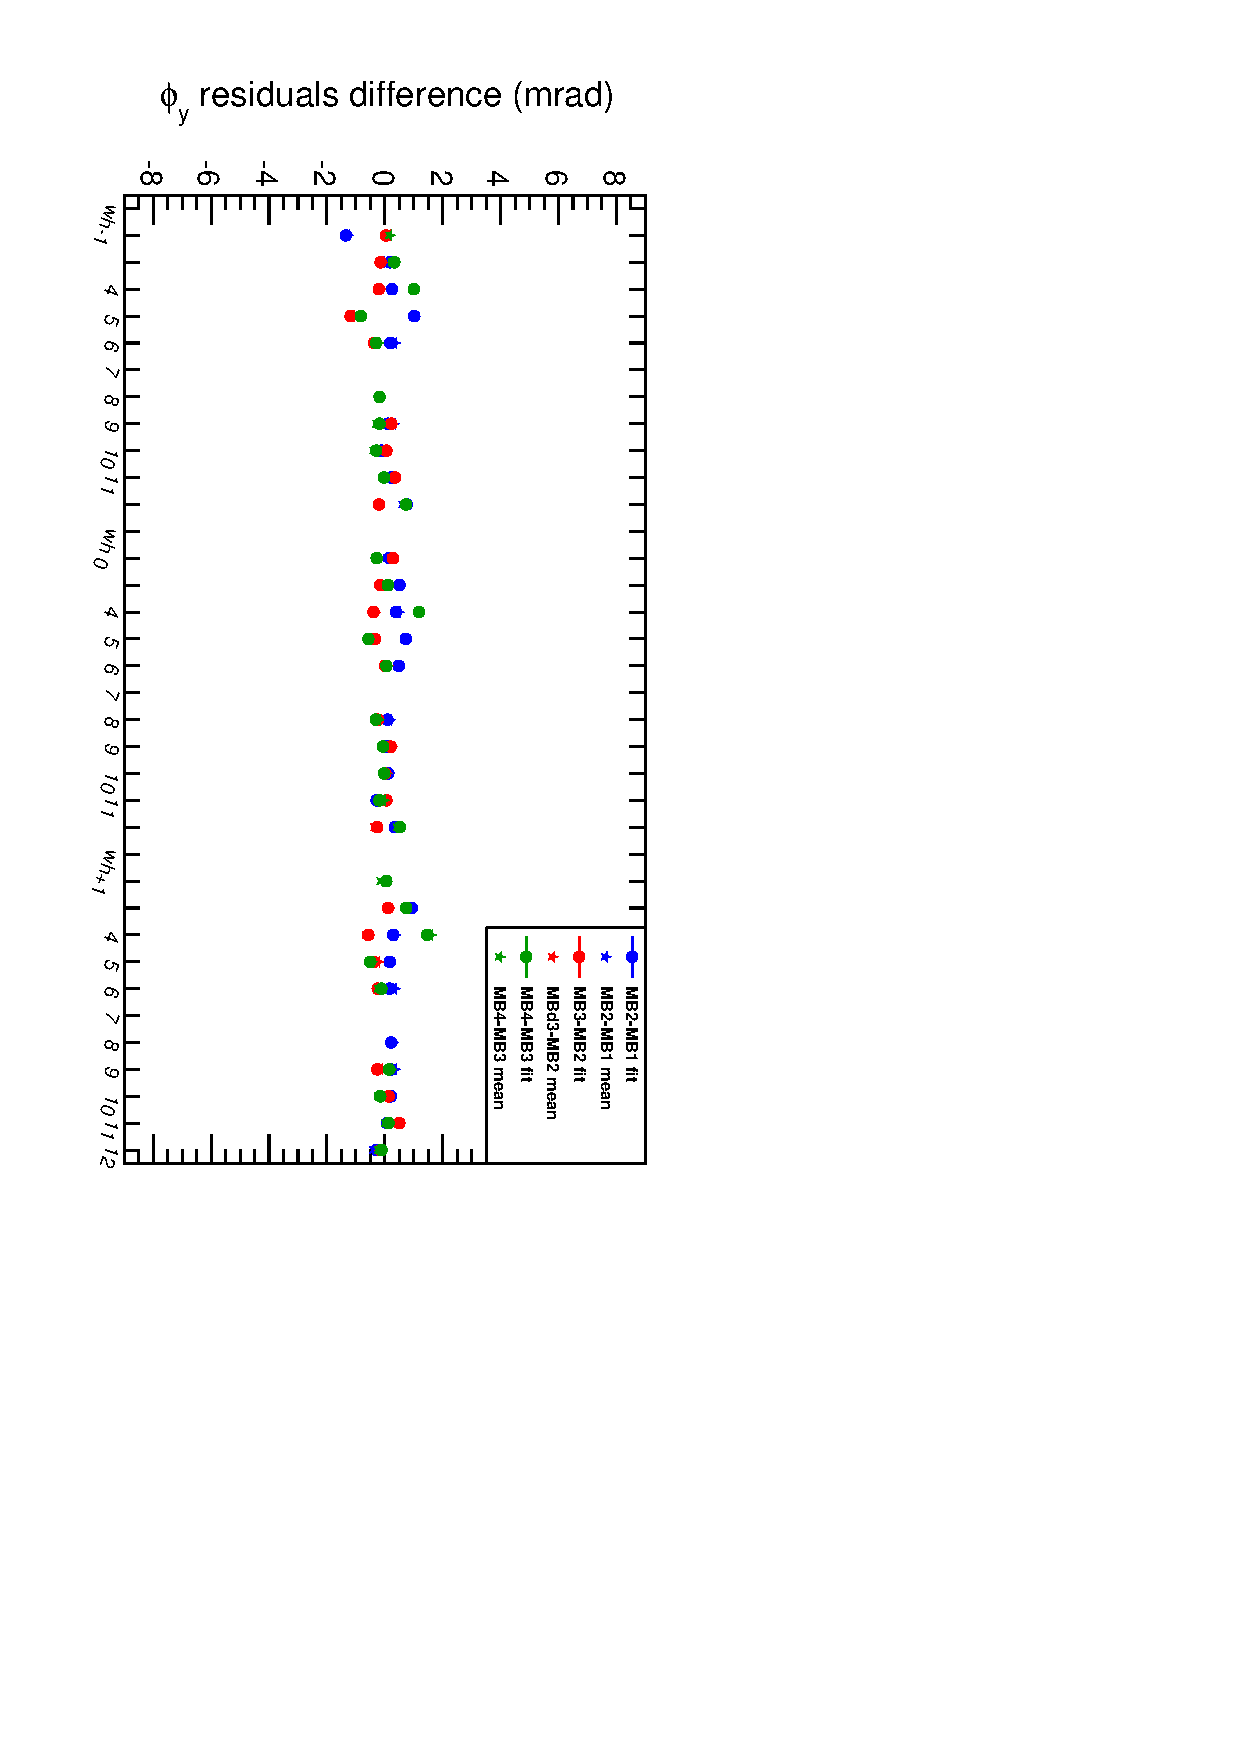
\includegraphics[width=4 cm, angle=90]{diffphisector_may25.pdf}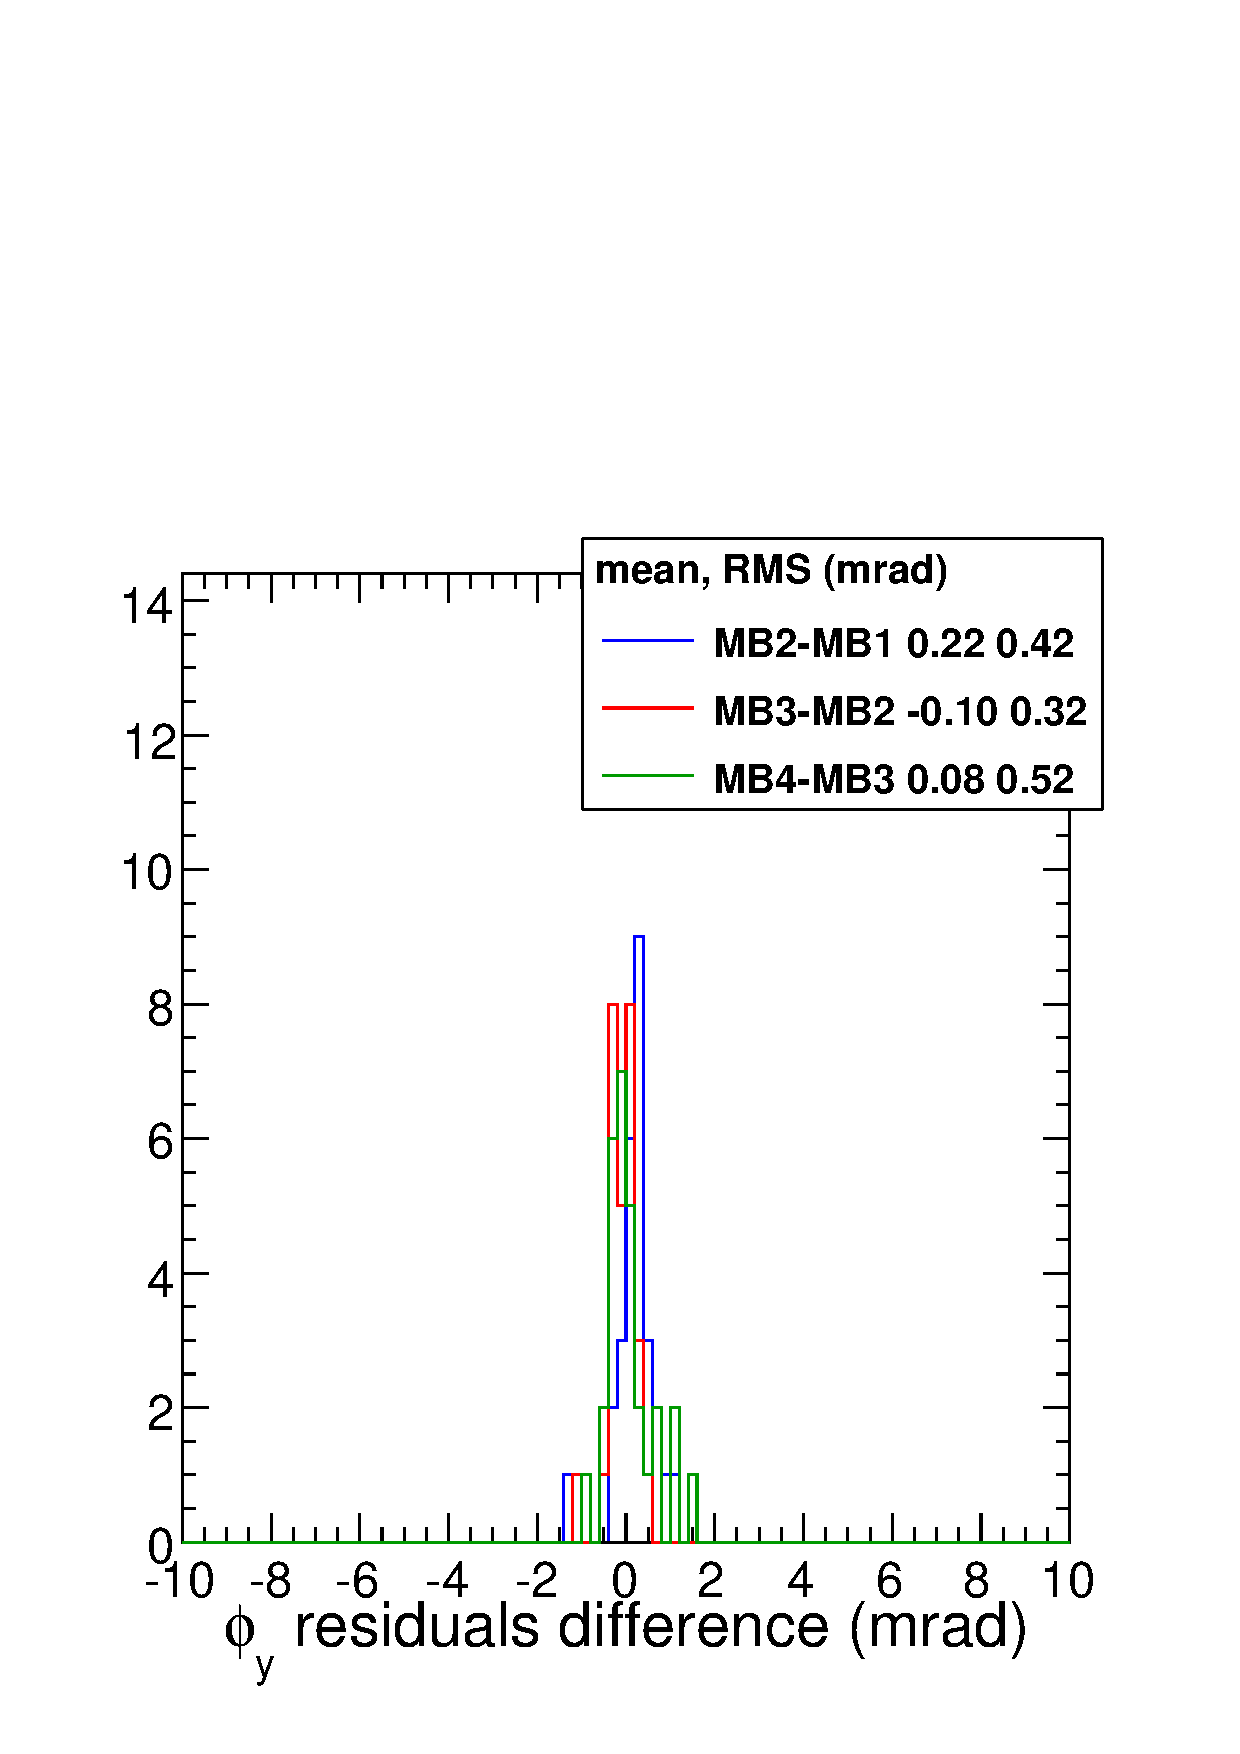
\includegraphics[height=4 cm]{diffphihist_may25.pdf}
\end{frame}

\begin{frame}
\frametitle{May 29 $x$}

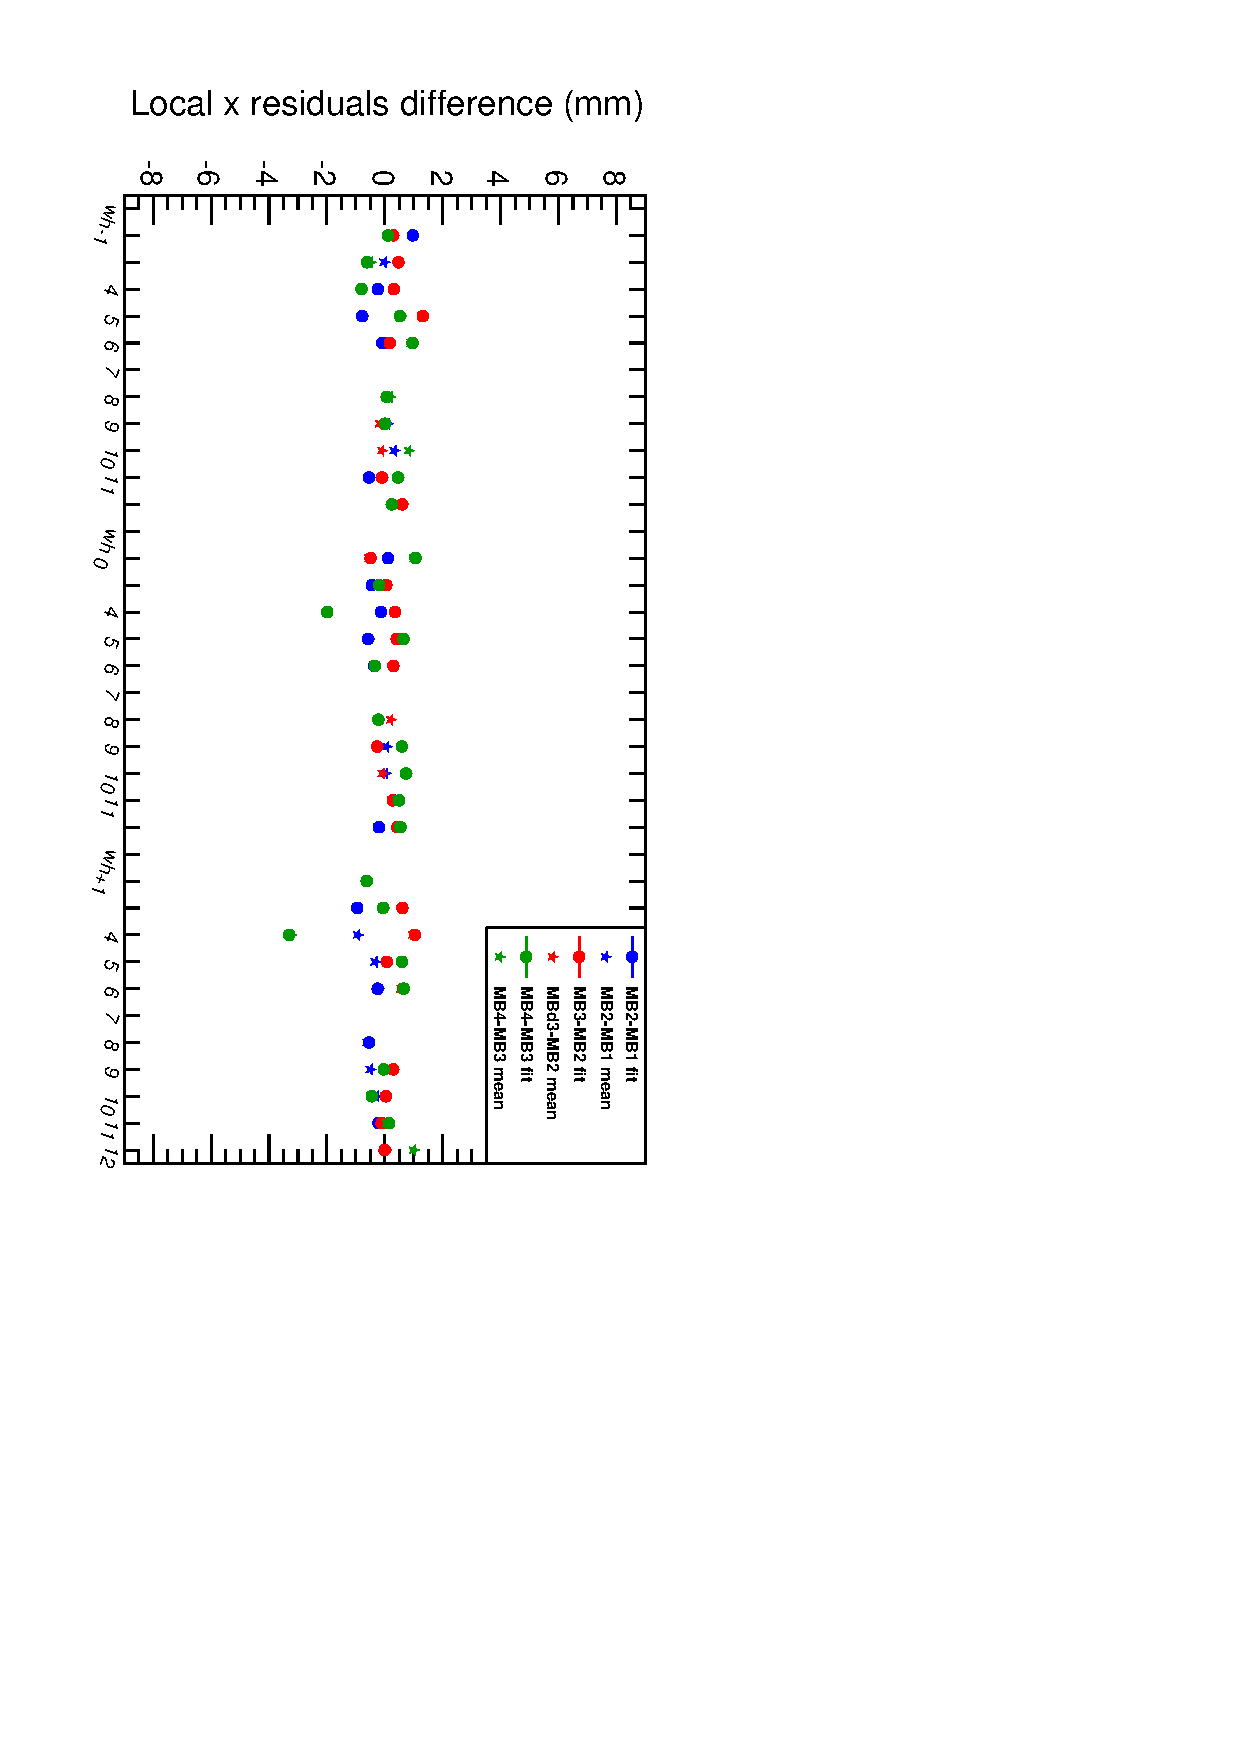
\includegraphics[width=4 cm, angle=90]{diffxsector_may29.pdf}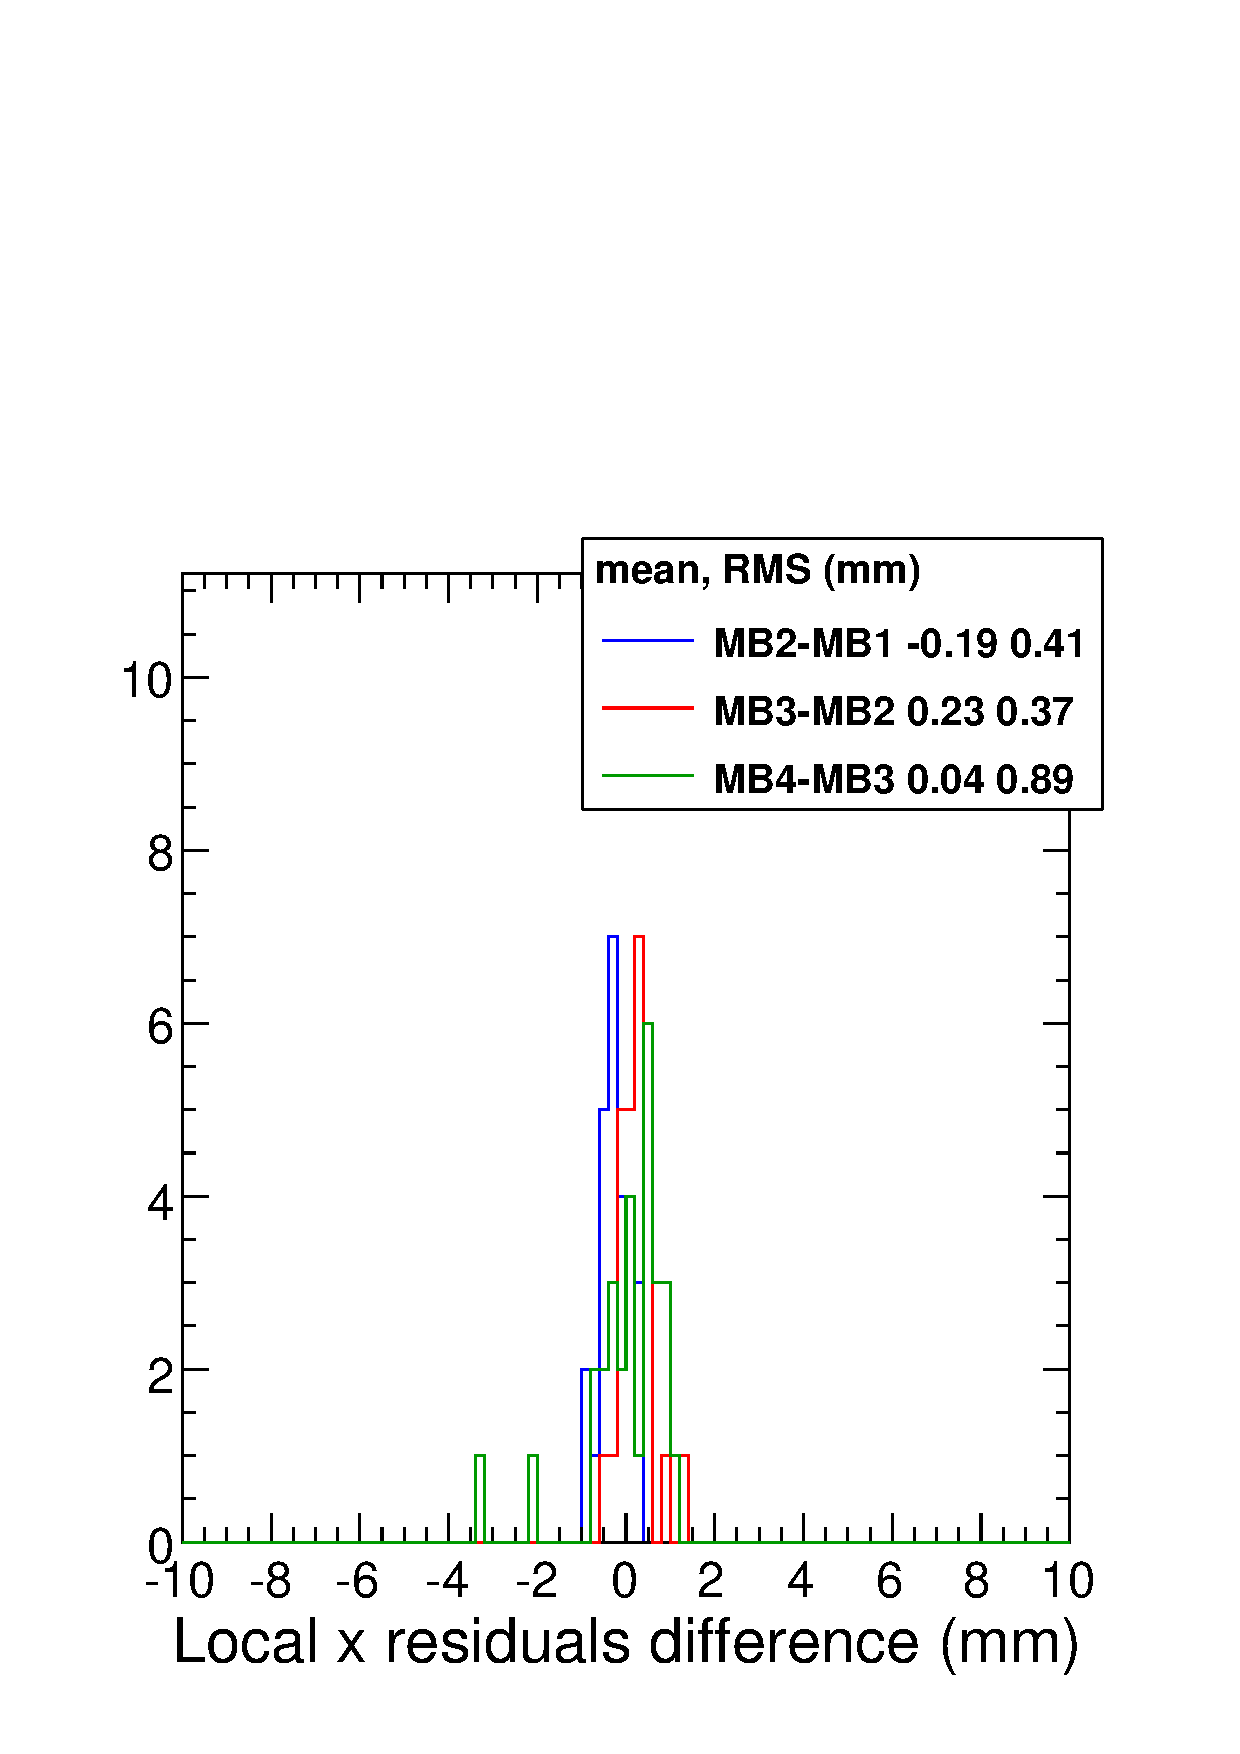
\includegraphics[height=4 cm]{diffxhist_may29.pdf}

\vfill
\hspace{-0.83 cm} \textcolor{darkblue}{\Large May 29 $\phi_y$}

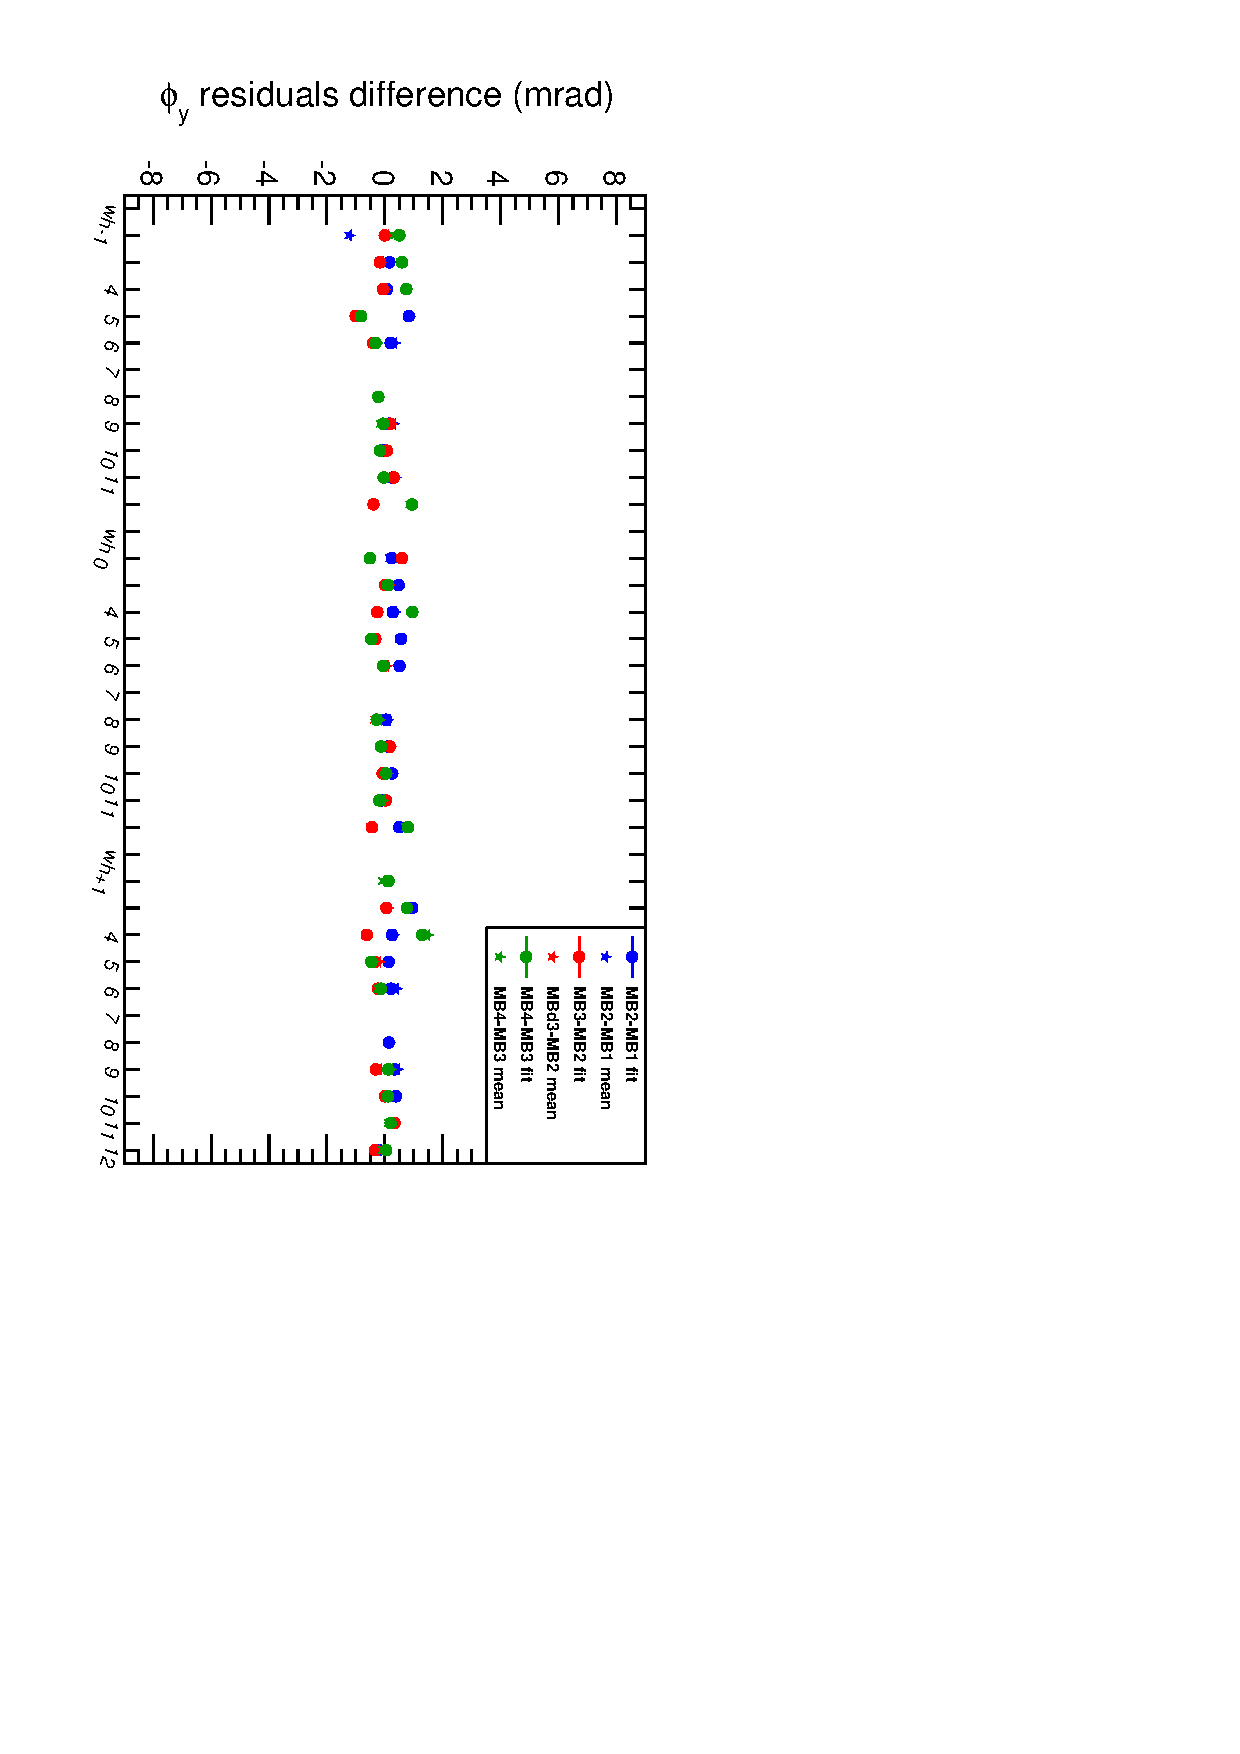
\includegraphics[width=4 cm, angle=90]{diffphisector_may29.pdf}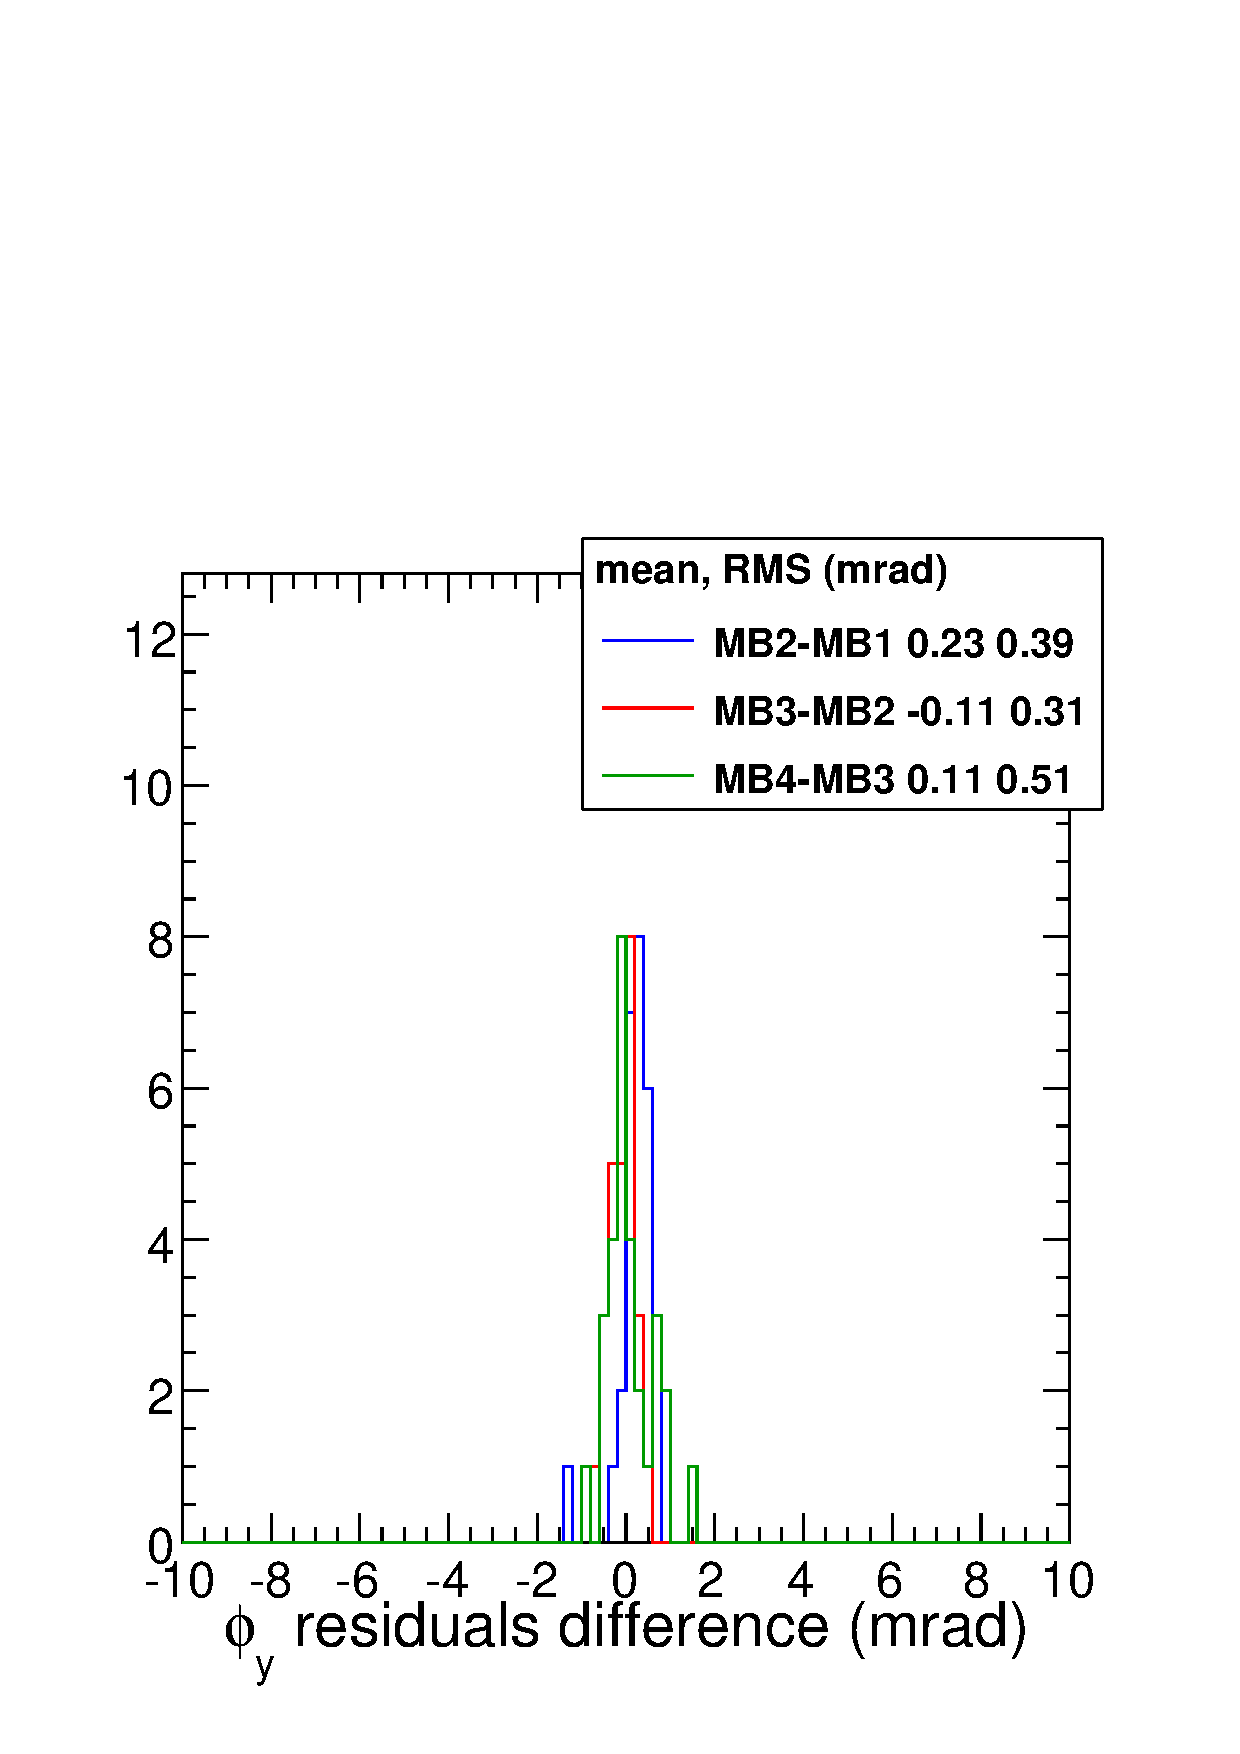
\includegraphics[height=4 cm]{diffphihist_may29.pdf}
\end{frame}

\begin{frame}
\frametitle{Comments}
\begin{itemize}
\item Chambers that were not included in a given alignment are not shown in the diagnostic:
\begin{itemize}
\item CRAFT\_ALL\_V4: not globalMuon alignment, all \mbox{chambers shown\hspace{-1 cm}}
\item CRAFT\_ALL\_V11: about half didn't pass the alignment criteria
\item May 25: wh$-$1 st2 sec8, wh$+$1 st2 sec2, wh$+$1 st3 sec8
\item May 29: wh$-$1 st2 sec8, wh$+$1 st2 sec2, wh$+$1 st3 sec8, wh$-$1 st1 sec12
\end{itemize}

\item The first time $\phi_y$ were corrected was after V11, so there
  are no V4-V11 differences in $\phi_y$ (just a masking of unaligned chambers)

\item DB-difference between May 25 and 29 in $\phi_y$ has an RMS of
  0.5~mrad; differences observed by tracks is also small

\item DB-difference between May 25 and 29 in $x$ has an RMS of
  2.5~mm; track-based difference is significant (and favors May 29)

\item Station~4, sector~4 chambers are often outliers in $x$, exactly
  as they were in the segment extrapolation plots.  These are also the
  chambers with internal structure (10~mm discontinuity in residuals
  at $x=0$ through the middle of the chamber).
\end{itemize}
\end{frame}

%% \begin{frame}
%% \frametitle{Outline}
%% \begin{itemize}\setlength{\itemsep}{0.75 cm}
%% \item 
%% \end{itemize}
%% %% \hspace{-0.83 cm} \textcolor{darkblue}{\Large Outline2}
%% \end{frame}

%% \section*{First section}
%% \begin{frame}
%% \begin{center}
%% \Huge \textcolor{blue}{First section}
%% \end{center}
%% \end{frame}

\begin{frame}
\frametitle{Conclusions}
\begin{itemize}\setlength{\itemsep}{0.5 cm}
\item Residuals differences, much like segment extrapolation,
  introduces new information, not used in alignment
\item With the exception of station~4 sector~4 chambers, relative
  differences in May 29 (latest) $x$ is 400~$\mu$m
\item Relative differences in $\phi_y$ are 0.3--0.5~mrad
\end{itemize}
\label{numpages}
\end{frame}

\end{document}
